\Chapter{Segmentation des lésions rétiniennes dans l'imagerie de \fundus{}.}\label{sec:Theme1}
\label{sec:ChapitreSegmentation}


Pour le médecin, l'identification et à la quantification des biomarqueurs visibles dans l'image de \fundus{} est un préalable au diagnostic des maladies affectant potentiellement la rétine. En effet, les règles diagnostiques d'un grand nombre d'entre elles se basent sur la reconnaissance d'une ou plusieurs structures anatomiques et de leur analyse (topologie, nombre, texture etc.). Parce qu'elle illustre parfaitement ce concept, prenons la rétinopathie diabétique comme exemple: chaque grade de la maladie est caractérisé par un ensemble de marqueurs (essentiellement des lésions) dont l'évolution (en taille, nombre et type) est révélatrice de la progression de la gravité de la maladie \cite{boucherEvidencebasedCanadianGuidelines2020}. En pratique, cette identification est loin d'être aisée, y compris pour des cliniciens expérimentés. Qui plus est, le recours de plus en plus fréquent aux centres de télé-dépistages privent l'examinateur d'informations contextuelles lui permettant de résoudre certaines ambiguïtés. Nous illustrons dans la section \ref{sec:segmentationDifficulte} suivante  plusieurs des difficultés pouvant tromper y compris l'\oeil{} expert. À ce titre, confier la tâche à un algorithme est perçue comme une solution potentielle. L'identification des frontières des structures locales et la reconnaissance de celles-ci dans une image est appelée segmentation sémantique. Ce chapitre traite de la question de l'obtention des cartes de segmentation pour chaque grande classe de lésions existante dans le \fundus{}, mais aussi de l'exploitation de ces segments une fois ces cartes obtenues.

À travers notre revue de littérature sur le sujet (section \ref{sec:segmentationFCCN})  se dessine l'image d'un champs de recherche actif et massivement tourné vers la conception et l'optimisation de nouvelles architectures de réseaux de neurones. Pour subvenir aux besoins de cette recherche, de plus en plus d'équipes ont mis en accès libre leurs données pour un usage académique, ce qui représente souvent l'équivalent de plusieurs centaines d'heures de travail d'annotations réalisées par des experts. En revanche, rares (sinon inexistants) sont les travaux qui explicitent leur protocole d'annotations de manière détaillée et reproductible. Cela mène à des annotations inter-bases très hétérogènes, bien que représentant supposément les mêmes structures. À cela s'ajoute que chaque base de données représente une certaine population et a été acquise dans des conditions spécifiques (caméra, condition d'éclairage, acquisition mydriatique ou non...). Or, étant donnée la taille relativement réduite de ces bases, il apparaît clairement qu'une représentation exhaustive de toutes les spécificités du \fundus{} à travers une seule base confine à la gageure. Pourtant, il n'existe à notre connaissance aucun travail cherchant à combiner ces bases de données (que ce soit pour entraîner ou évaluer un modèle) ou même simplement à les caractériser respectivement. La littérature tend globalement à décorréler les travaux sur la segmentation en elle-même et les questions afférentes à la généralisation.
L'étude présentée dans ce chapitre propose donc de combler cette absence d'analyse comparative. Plusieurs objectifs de recherche vont venir préciser et élargir largement l'ambition initiale de ce travail et sont détaillés dans la section \ref{sec:SegmentationProblematique}. Pour délimiter notre étude, le choix a été fait de ne considérer que les cinq bases de données récentes les plus importantes. Par ordre de taille (i.e. de 
nombre d'images) celles-ci sont:
\begin{enumerate}
	\item \acf{IDRiD}\cite{porwalIDRiDDiabeticRetinopathy2020}.
	\item MESSIDOR \cite{decenciereFEEDBACKPUBLICLYDISTRIBUTED2014b}
	\item \acf{DDR} \cite{liDiagnosticAssessmentDeep2019a}
	\item RET-LES \cite{weiLearnSegmentRetinal2021}
	\item \acf{FGADR} \cite{zhouBenchmarkStudyingDiabetic2021}
\end{enumerate}
Une description détaillée de ces bases est proposée dans la section \ref{sec:variabilitéSegmentation}.
Ces jeux de données ont l'avantage d'avoir en commun certaines annotations de lésions spécifiques, sur lesquelles porte notre travail:
\begin{enumerate}
	\item \acf{EX} (également qualifiés d'\textit{exsudats durs})
	\item \acf{HEM}
	\item \acf{MA}
	\item \acf{CWS}
\end{enumerate}

Notre étude s'arrime donc à la tendance de la majorité des articles publiés qui se restreint à ces quatre lésions. Notons qu'il existe des travaux étendant leur portée à un plus grand nombre de lésions; en particulier pour la segmentation des ischémies et des néo-vascularisations \cite{weiLearnSegmentRetinal2021}, qui sont de toute première importance pour la classification des stades avancées de la rétinopathie \cite{boucherEvidencebasedCanadianGuidelines2020}. Mais notre étude se voulant comparative, il était nécessaire de se limiter au dénominateur commun en terme de classes traitées.


\subsection{Difficultés liées à la segmentation des lésions}
\label{sec:segmentationDifficulte}
Il est notoire - et les efforts continus de recherche en attestent- que la segmentation des lésions rétiniennes n'est pas une tâche aisée; même en faisant abstraction des difficultés liées à la disparité entre les bases de données. Nous recensons sur la figure \ref{fig:DifficultesAcquisition} un certain nombre de cas illustrant la complexité du problème, toutes les images étant issues de la même base RET-LES.  
\begin{figure}
	\begin{subfigure}[t]{.5\textwidth}
		\includegraphics[width=\textwidth]{segmentation_lesions/difficultees/cil.png}
		\caption{Artefacts visibles dans la région inférieure (cils)}
	\end{subfigure}
	\begin{subfigure}[t]{.5\textwidth}
		\includegraphics[width=\textwidth]{segmentation_lesions/difficultees/surexposition.png}
		\caption{Sur-exposition lumineuse qui sature le champ temporal de la rétine}
	\end{subfigure}
	\begin{subfigure}[t]{.5\textwidth}
		\includegraphics[width=\textwidth]{segmentation_lesions/difficultees/sombre.png}
		\caption{Sous-exposition globale compliquant la lecture de la périphérie temporale supérieure de la rétine}
	\end{subfigure}
	\begin{subfigure}[t]{.5\textwidth}
		\includegraphics[width=\textwidth]{segmentation_lesions/difficultees/faible_contraste.png}
		\caption{Faible contraste dans le champ nasal due à une pathologie (détachement rétinien ou cataracte)}
	\end{subfigure}
\caption{Images issues de la base de données RET-LES.}
\label{fig:DifficultesAcquisition}
\end{figure}

Nous avons également eu l'occasion de vérifier cette difficulté liée à l'identification des lésions en conduisant également une micro-étude auprès de trois experts de la rétine. Nous leur avons demandé de faire la gradation de la rétinopathie diabétique sur 200 images ainsi que l'identification de la présence d'\oe dème maculaire, suivant une échelle classique de 0 à 4. Il en ressort notamment douze images (6\%), pour lesquelles il existe un désaccord total entre les trois observateurs (c'est-à-dire qu'aucune paire ne s'accorde). Après révisions une-à-une des images en session, le désaccord s'avéra porter sur l'identification de certaines structures en tant que lésions de type micro-anévrismes. Or, sur cinq des douze images, une poussière sur le capteur de la caméra, visible dans la région maculaire, a trompé deux des trois observateurs sur la présence d'un micro-anévrisme. Le dernier observateur a constaté la présence de cette anomalie en comparant la position (toujours identique) de ce faux anévrisme sur ces 5 images consécutivement.
\\ 
Cette anecdote témoigne du type de difficultés existant dans la segmentation rétinienne et du défi qu'elle représente y compris pour des experts humains.
\subsection{Variabilité inter-bases}
\label{sec:variabilitéSegmentation}
Les cinq bases de données que nous analysons font état d'importantes inter-disparités à deux niveaux:
\begin{itemize}
	\item En terme d'images en elles-mêmes; les facteurs de variabilité étant l'apparence de l'image (terme générique regroupant la colorimétrie, le contraste, l'exposition...), la résolution, la qualité d'acquisition et la diversité des symptômes des patients présents dans la base.
	\item En terme d'annotations réalisées par les médecins; cette fois, ce sont la finesse (c'est-à-dire la précision aux frontières) des annotations,  leur quantité et le nombre de classes différentes annotées qui font cette diversité.
\end{itemize}
Bien entendu, à cela s'ajoute que les bases de données sont de taille diverses. Le tableau \ref{tab:databasesCaracteristics} fournit le détail de la composition de chaque base.
\begin{table}
	\centering
	\caption{Composition de chacune des bases de données utilisées. \acf{HIV}, \acf{HIR}, \acf{HPR}, \acf{IrMA}, \acf{NV}}
	 \rowcolors{2}{white}{gray!10}
	\begin{tabularx}{\linewidth}{llcX}
		\toprule
		Bases & Nombre d'images & Résolution & Classes annotées \\
		\midrule
		\ac{IDRiD} & 81 & $2848 \times 4288$ & \ac{MA}, \ac{HEM}, \ac{CWS}, \ac{EX}\\
		MESSIDOR & 200 & $1500\times 1500$ & \ac{MA}, \ac{HEM}, \ac{CWS}, \ac{EX}, Drusen, Macula, Disque Optique, Coupe Optique, \ac{HPR}, \ac{NV}, Vaisseaux Sanguins\\		
		\ac{DDR} & 757 & $1934 \times 1956$ & \ac{MA}, \ac{HEM}, \ac{CWS}, \ac{EX}\\
		RET-LES & 1593 & $896 \times 896$ & \ac{MA}, \ac{HEM}, \ac{CWS}, \ac{EX}, \ac{NV}, \ac{HIV}, \ac{HIR}, Prolifération Fibreuse\\
		\ac{FGADR} & 1842 & $1280 \times 1280$ & \ac{MA}, \ac{HEM}, \ac{CWS}, \ac{EX}, NV, IRMA\\		
		\bottomrule
	\end{tabularx}

\label{tab:databasesCaracteristics}
\end{table}

La variabilité statistique des annotations dépend grandement du protocole d'annotation, sur lequel nous n'avons en général que peu d'informations. Or, la variabilité qu'il induit est très important: nous en proposons une estimation quantifiable sur la figure \ref{fig:annotationsManuellesBases}.
La finesse des annotations d'une base comme \ac{IDRiD} suggère une assistance par ordinateur pour faciliter un marquage extrêmement détaillé. Nous pouvons attester que cette stratégie est utilisée sur MESSIDOR, le processus d'annotations ayant été réalisé dans le cadre de ce doctorat en collaboration avec des cliniciens ayant vérifié et corrigé les annotations pré-réalisées automatiquement par un modèle.
Inversement, sur RET-LES, les annotations suggèrent un tracé à la main à partir de formes géométriques simples pré-définies. Entre ces deux extrêmes, les styles varient: comme on peut le voir sur la colonne correspondant à \ac{FGADR}, celle-ci présente à la fois des annotations aux frontières fines (trois premières lignes) et plus grossière (quatrième ligne).

\newcommand{\colSize}{0.19}
\begin{figure}
	\centering
	\begin{subfigure}{\colSize\textwidth}
		\includegraphics[width=\textwidth]{segmentation_lesions/distributions_labels/idrid.png}
		\caption{IDRID}
	\end{subfigure}
\begin{subfigure}{\colSize\textwidth}
	\includegraphics[width=\textwidth]{segmentation_lesions/distributions_labels/messidor.png}
	\caption{MESSIDOR}
\end{subfigure}
\begin{subfigure}{\colSize\textwidth}
	\includegraphics[width=\textwidth]{segmentation_lesions/distributions_labels/ddr.png}
	\caption{DDR}
\end{subfigure}
\begin{subfigure}{\colSize\textwidth}
	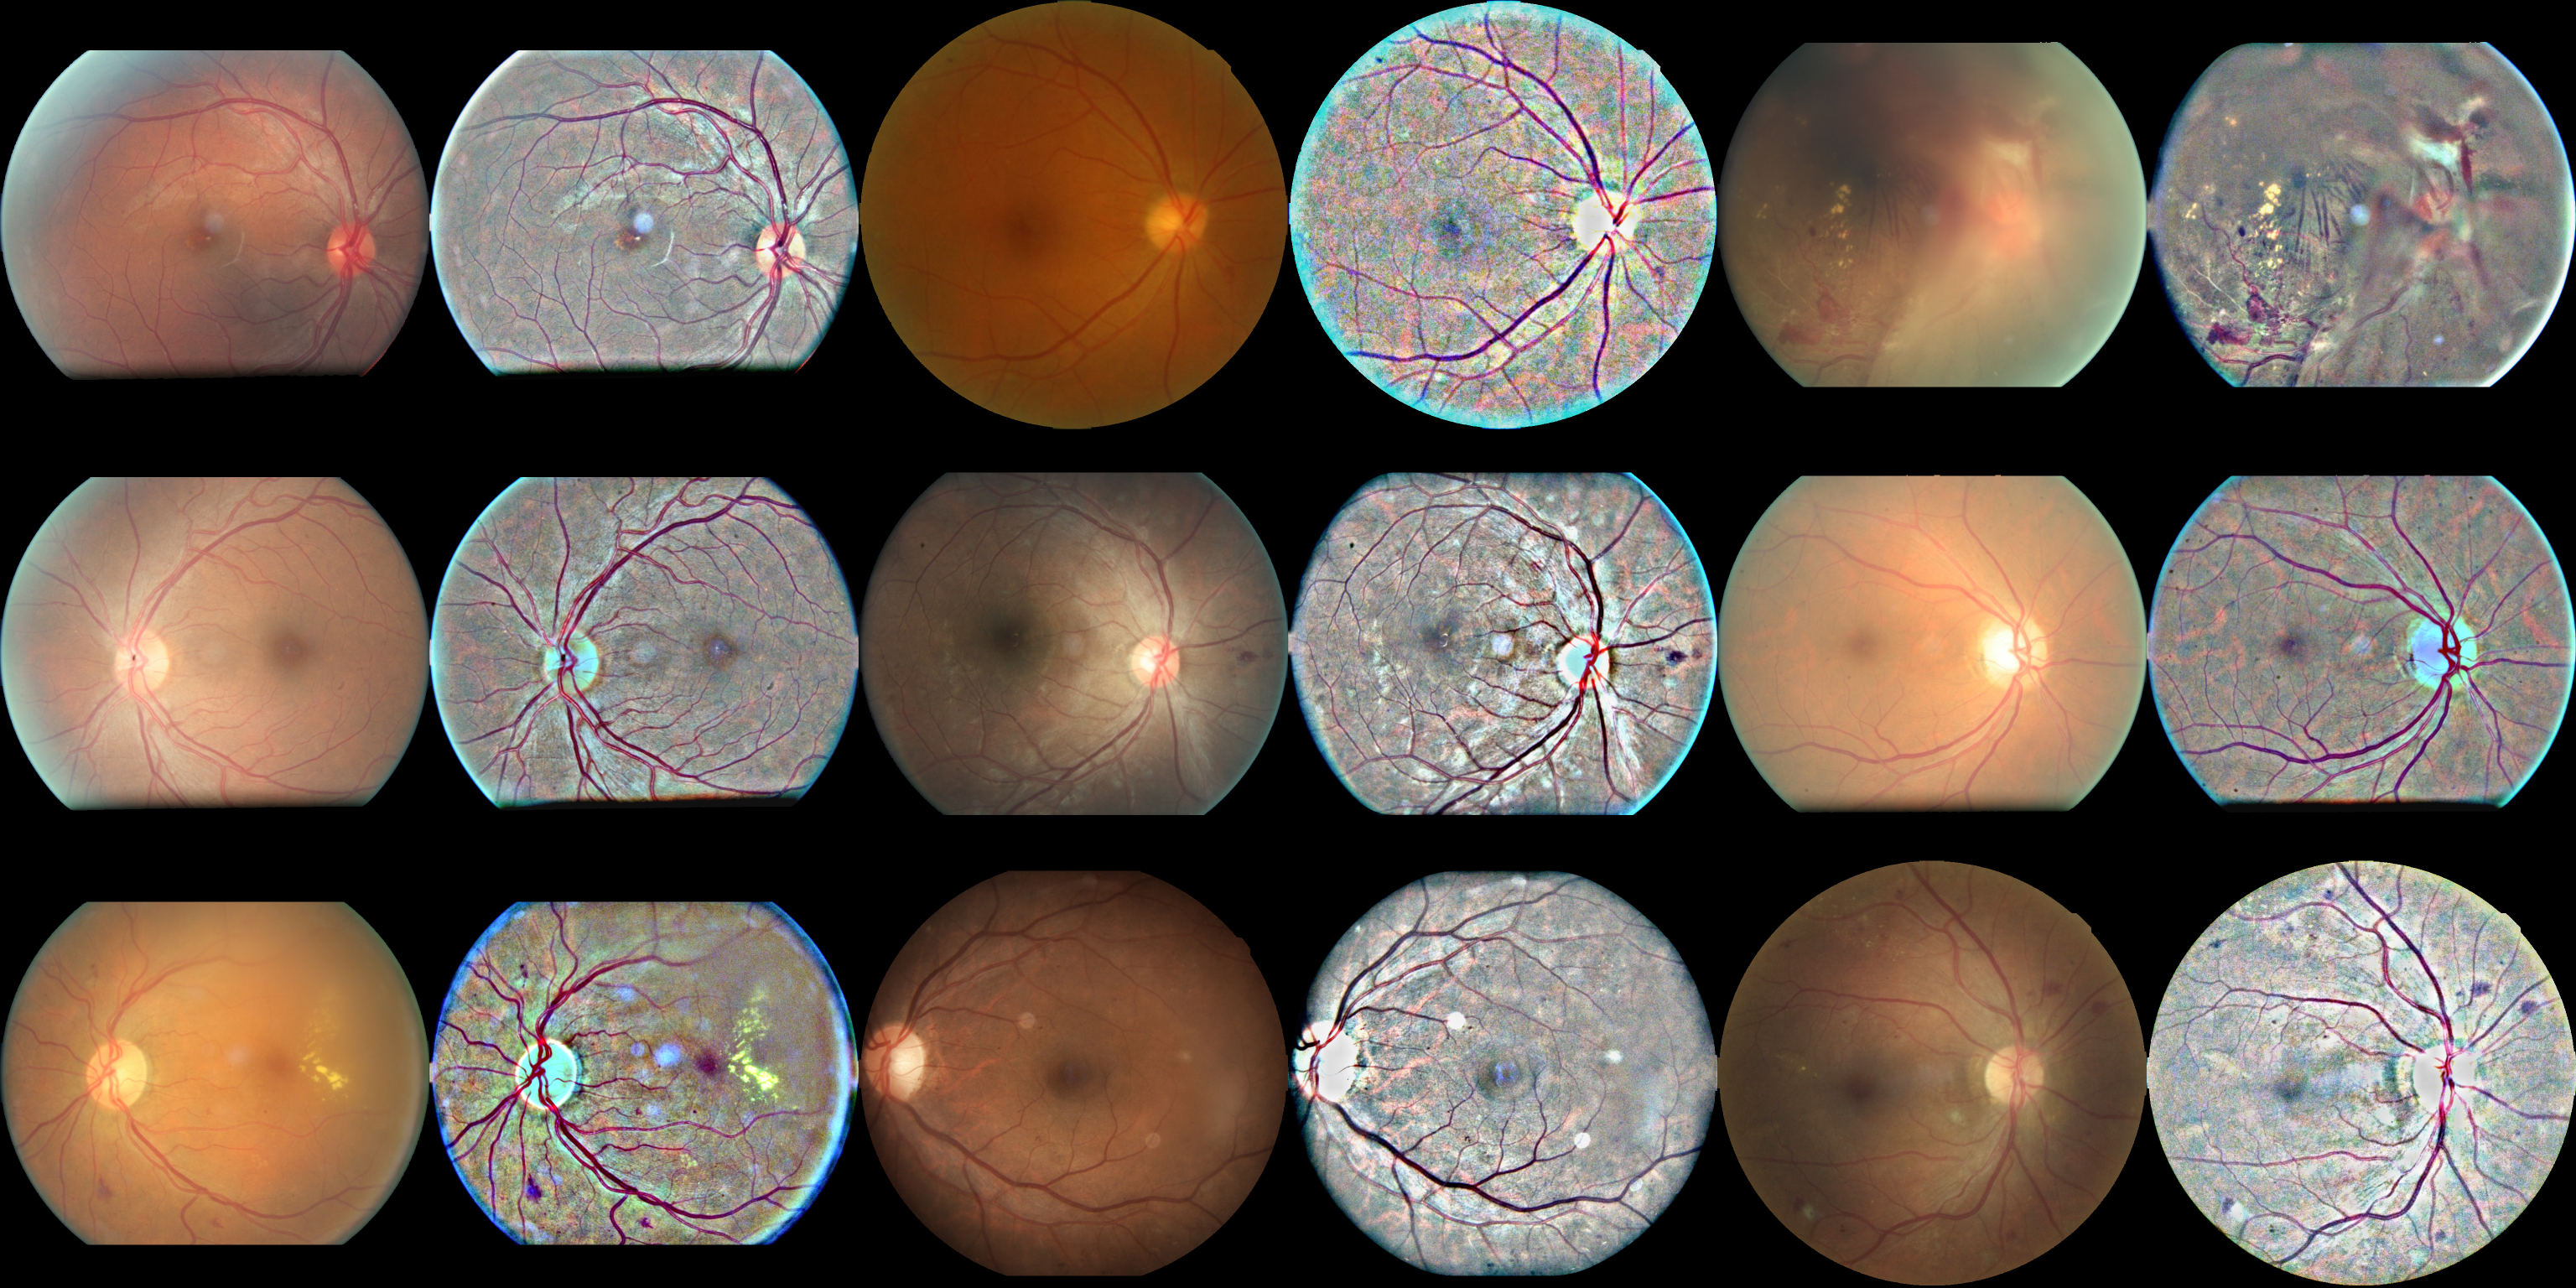
\includegraphics[width=\textwidth]{segmentation_lesions/distributions_labels/RETINAL_LESIONS.png}
	\caption{RET-LES}
\end{subfigure}
\begin{subfigure}{\colSize\textwidth}
	\includegraphics[width=\textwidth]{segmentation_lesions/distributions_labels/fgadr.png}
	\caption{FGADR}
\end{subfigure}
\caption{Images accompagnées de leurs annotations manuelles organisées suivant leur base d'appartenance. Que ce soit dans les couleurs, le découpage de la région d'intérêt ou les annotations, on constate une grande variabilité inter et intra base.}
\label{fig:annotationsManuellesBases}
\end{figure}
Il est possible de se faire une idée plus quantifiée du style d'annotations propre à chaque base. Pour cela, on propose une analyse statistique de la distribution jointe du nombre de lésions et de leur taille moyenne par image. Bien entendu, ces deux variables dépendent du diagnostic de la maladie sous-jacente, mais ici toutes les images considérées sont pathologiques (à des degrés de sévérité divers). Abstraction donc faite de la maladie, la seconde dépendance entre ces variables vient du style d'annotation. En particulier, deux régimes se distinguent: pour une annotation de granularité fine, l'expert aura tendance à marquer de nombreux éléments de manière précise et détaillée. Inversement, une annotation plus grossière aura tendance à fusionner ensemble les structures locales voisines en des structures plus grosses et moins nombreuses. La figure \ref{fig:jointDistributionLesion} montre ces distributions jointes pour les quatre lésions et pour chacune des cinq bases de données. Elle met bien en évidence l'observation qualitative: \ac{IDRiD} se distingue par un grand nombre d'éléments segmentés de petite taille, suivi généralement de \ac{DDR} et MESSIDOR. RET-LES est systématiquement la moins fine, toutes lésions confondues (celles-ci étant moins nombreuses et de plus grande taille). Enfin, tel que visible sur la figure \ref{fig:annotationsManuellesBases}, FGADR se retrouve à cheval entre ces deux tendances, présentant des images possédant de nombreuses lésions de petites tailles et d'autres en possédant peu mais de grandes tailles. 

\begin{figure}
	\begin{subfigure}{.5\textwidth}
		\includegraphics[width=\textwidth]{segmentation_lesions/distributions_labels/Cotton_Wool_Spot.png}
		\caption{Distribution des \ac{CWS}}
	\end{subfigure}
	\begin{subfigure}{.5\textwidth}
		\includegraphics[width=\textwidth]{segmentation_lesions/distributions_labels/Exudates.png}
		\caption{Distribution des \ac{EX}}
	\end{subfigure}
	\begin{subfigure}{.5\textwidth}
		\includegraphics[width=\textwidth]{segmentation_lesions/distributions_labels/Hemorrhages.png}
		\caption{Distribution des \ac{HEM}}
	\end{subfigure}
	\begin{subfigure}{.5\textwidth}
		\includegraphics[width=\textwidth]{segmentation_lesions/distributions_labels/Microaneurysms.png}
		\caption{Distribution des \ac{MA}}
	\end{subfigure}
\caption{Représentation des distributions jointes de la taille moyenne et du nombre de lésions par images pour chaque classe. Les croix représentent les centroïdes de chaque distribution. Pour pouvoir représenter les distributions sur un même graphique, il a fallu choisir une échelle logarithmique, il y a donc plusieurs ordres de grandeur séparant les centroïdes.  En comparant les bases de données, on met ainsi en évidence la disparité des styles d'annotations entre chacune.}
\label{fig:jointDistributionLesion}
\end{figure}


\section{Problématique}
\label{sec:SegmentationProblematique}
Considérant les éléments relatifs aux deux sections précédentes (c'est-à-dire les difficultés liées à la segmentation et la grande variabilité inter-base existante), plusieurs éléments de problématique se posent: 
\begin{itemize}
	\item Quelles sont les capacités de généralisation d'un modèle donné sur diverses bases de données?
	\item Corollairement, que peut-on conclure des performances d'un modèle à partir d'une seule base?
	\item Quel impact le style d'annotations propre à chaque base va-t-il avoir sur le diagnostic de la pathologie?
\end{itemize}
À travers les deux premières questions, nous dressons un premier objectif de recherche, qui est de concevoir un modèle capable de segmenter plusieurs lésions simultanément. Nous ajoutons deux contraintes techniques sur le choix du modèle: celui-ci doit pouvoir être facilement reproductible (donc sans ambiguïté d'implémentation) et ses performances doivent a minima égaler les modèles de l'état de l'art. Ce modèle nous servira de base pour évaluer les problématiques de généralisation.
\\
Notre second objectif de recherche porte sur l'évaluation de la capacité de généralisation empirique du modèle sur différentes bases afin de dresser le tableau des compatibilités inter-bases. \\
Une question de recherche vient se greffer à cet objectif, qui est celle de la pertinence des métriques utilisées pour l'évaluation de la qualité de la segmentation. Pour répondre à ce questionnement, un autre axe d'analyse sera traité, qui décrit la relation entre qualité de la segmentation et de détection des lésions. 
\\
En vue d'uniformiser les performances inter-bases, il est assez intuitif de vouloir réduire la variabilité entre les images présentées par un effet de prétraitement. Nous proposons d'explorer l'effet qu'induit un tel type de traitement sur le modèle.
\\
Nous nous attendons à trouver des disparités au sein des modèles de segmentation dépendamment de leur base d'entraînement. Notre objectif principal est à la fois d'en étudier les conséquences en terme de segmentation sur des images de test mais aussi de proposer une méthode pour contrôler le comportement des modèles en fonction du besoin clinique. On notera cependant que celui-ci n'est pas clairement défini:
dans quelle mesure ces disparités de segmentation sont-elles cliniquement pertinentes ou dommageables? \\
Pour clarifier cette question, nous proposons dans un dernier temps d'étudier la capacité d'un modèle à classifier une image à partir des lésions identifiées en elle. 

\section{Méthodologie}
Notre méthodologie s'articule autours de quatre axes, dont chacun fait l'objet d'une section dans la partie qui suit:
\begin{enumerate}
	\item La standardisation via des traitements algorithmiques simples des images d'entrée.
	\item La conception d'une architecture de segmentation, incluant sa comparaison avec l´état de l'art.
	\item La mise en place d'une stratégie permettant d'uniformiser les performances d'un modèle à travers plusieurs distributions de données.
	\item Le développement d'un modèle de classification permettant l'évaluation de la pertinence de la segmentation à des fins diagnostiques.
\end{enumerate}
\subsection{Normalisation des données}
Les images utilisées varient en résolution et en apparence. La phase de prétraitement vise donc à corriger ces deux aspects et est présentée dans cette section. La standardisation des résolutions est une nécessité technique, notamment du fait que les modèles ne sont théoriquement pas invariants en échelle; elle est donc menée pour chacune de nos expériences. En revanche, l'intérêt de l'homogénéisation de l'apparence est plus discutable. Pour alléger ce chapitre et à la vue de résultats mitigés, nous le mentionnons brièvement dans la section \ref{sec:preprocessingQuick} mais le détail des résultats est reporté en annexe \ref{an:PrétraitementDonnées}.
\subsubsection{Standardisation des résolutions}
\label{sec:resolution_standardisation}
La résolution d'image varie dépendamment de la base. Afin de standardiser le format d'entrée de nos modèles, notre protocole inclut les étapes suivantes:
\begin{enumerate}
	\item La région d'intérêt (rétine) est extraite. Pour cela, on utilise un simple effet de seuillage sur le canal rouge de l'image.
	\item L'image est ensuite découpée pour éliminer les bordures noires et ainsi être centrées sur la région d'intérêt.
	\item Si l'image résultante n'est pas de format carrée, on utilise du \textit{padding} (complétion des bords par des zéros) sur la dimension la plus petite pour lui conférer ce format.
	\item L'image est ensuite redimensionnée au standard que nous avons adopté de $1536 \times 1536$.
\end{enumerate}
On peut noter que cette résolution est supérieure à celle des images fournies dans RET-LES et FGADR. Pour ces deux bases, les images apparaîtront comme légèrement moins détaillées (la sous-résolution initiale pouvant agir comme un filtre passe-bas). En pratique, nous avons quantifié cet effet, en utilisant des images de très hautes résolutions (type IDRID), filtrées par un passe-bas pour simuler une sous-résolution. Nous n'avons pas observé de changements drastiques de comportement des CNNs entraînés dépendamment de ce filtrage, ce qui semble légitimer la sur-résolution de toutes les bases au standard que nous avons adopté. Précisons tout de même que la résolution choisie reste exceptionnellement élevée: dans la littérature, la plupart des modèles sont entraînés sur des images de taille $512 \times 512$. Plusieurs travaux font cependant état d'une corrélation entre qualité du dépistage et résolution des images, il paraît donc pertinent d'adopter un standard élevé pour celle-ci.
\subsubsection{Algorithme de prétraitement}
\label{sec:preprocessingQuick}
La nécessité et l'impact d'un prétraitement des données -visant à homogénéiser l'apparence des images indépendamment de leur origine- sont encore très débattus dans la littérature. Nous avons mené nos propres expériences en la matière. Le protocole et les résultats détaillés sont fournis en annexe \ref{an:PrétraitementDonnées} mais en voici les conclusions résumées:  quel que soit l'angle d'analyse choisi (par lésions ou par bases de données), les gains potentiels obtenus par un traitement visant à normaliser l'apparence des images semblent limités. En revanche, il existe des cas pour lesquels ils entraînent des situations de faillite complète de convergence du modèle mais nous n'avons pas exploré les raisons expliquant ces configurations défectueuses. Pour la suite du chapitre, nous considérons donc les images dans leur apparence initiale, sans algorithme de prétraitement.

\subsection{Conception d'une architecture polyvalente}
\label{sec:segConceptionArchitecture}
Le choix d'une architecture de réseau de neurones est sujet à de nombreuses considérations sur les données et le budget calculatoire disponible. De nombreux travaux sur la segmentation du \fundus{} mettent en avant (voir la revue de littérature en section \ref{sec:segmentationFCCN}) la grande variabilité de taille des lésions et proposent des modèles combinant une approche locale et globale pour la prendre en compte. Mais en pratique, notre revue de littérature ne fait pas ressortir une architecture indiscutablement plus performante que les autres, trop de variables (nombre de paramètres, résolution d'images, prétraitement, itérations d'entraînement) étant interdépendantes sans qu'il n'y ait de consensus sur leur importance respective. De plus, les variations de performances sont souvent relativement minimes, qui plus est sur des métriques bien précises et potentiellement sensibles à des micro-variations (par exemple dues aux frontières de segmentation, par nature ambiguës). On observe également souvent une absence de standard dans le rapport fourni des résultats, que ce soit sur le choix de la métrique ou son mode de calcul. Heureusement, des concours comme \ac{IDRiD} ont permis de corriger cet aspect dans une certaine mesure, standardisant l'utilisation de certaines métriques et facilitant ainsi les comparaisons. Enfin, pour l'essentiel de la littérature, on note que seules les performances de segmentation sont rapportées et non celles de détection. Or, aucun travail ne semble s'interroger sur la pertinence d'une segmentation fine d'un point de vue diagnostic par rapport à une simple détection: autrement dit, la précision sur les frontières de segmentation n'a, pour l'heure, pas démontré sa pertinence clinique. 
\\
En dressant cet inventaire des freins à la comparaison à l'état de l'art, on dessine en creux une critique d'une tendance assez fréquente: celle de voir apparaître de nouvelles architectures introduites sans prendre en compte l'existant et la modularité des réseaux de neurones existants. Nous arguons qu'en l'absence de consensus sur ce qui fait la performance pratique d'un modèle, il est relativement superflu de se concentrer sur la construction de nouvelles architectures spécifiques au \fundus.
\\
Au contraire, nous suggérons d'utiliser la modularité des réseaux de neurones, qui nous permet d'obtenir une pléthore de combinaisons parmi les architectures existantes. Ces modèles ont l'avantage d'avoir été largement étudiés et éprouvés dans la littérature sur des bases de données généralistes autrement plus grandes et diverses. Par ailleurs, ces modèles sont plus facilement reproductibles, y compris dans leur version pré-entraînée car nous les avons extraits de librairies publiques connues.
 \\
Pour appuyer notre propos et afin de sélectionner l'architecture qui nous servira à conduire notre étude de généralisation, nous proposons d'explorer les forces de cette modularité architecturale, en combinant différent blocs. Toutes les architectures testées fonctionnent sur un même modèle de type:
\begin{equation}
	y = \mathcal{D}(\mathcal{E}(x))
\end{equation}
où $x, y$ sont respectivement les entrées et les sorties du modèle, $\mathcal{E}$ représente un module d'encodage et $\mathcal{D}$ de décodage. L'encodeur produit une ou plusieurs cartes de caractéristiques à différentes résolutions et le décodeur a la tâche de les combiner en une unique carte de segmentation. À partir de cette description simple, nous pouvons piocher dans la littérature pour concevoir séparément nos modules d'encodage et de décodage en respectant des structures d'architectures existantes. Le tableau \ref{tab:segmentationNetworks} reporte l'ensemble des combinaisons essayées. Le fonctionnement des différents modules sont décrits dans la section \ref{sec:FCCN}. Certains modules ne sont pas compatibles entre eux (ce qui explique les cases vides du tableau). En considérant ceux-ci, on aboutit à un total de 27 architectures comparées.
Cela nous permet de couvrir une large gamme de modèles, à la taille et à la complexité très variables. Notons que tous les modèles ne sont pas convolutifs, en particulier, les encodeurs MIT B2/4 se basent sur l'architecture du SegFormer (utilisant des réseaux auto-attentifs).

\begin{table}
	\centering
	\caption{Architectures utilisées dans notre étude comparative, accompagnées de leur taille (paramètres et FLOPs)}
	\label{tab:segmentationNetworks}
	\begin{tabularx}{\textwidth}{Xlcc}
		\toprule
		Architecture & Encodeur & \# Paramètres & \# FLOPs \\
		\midrule
		\multirow{8}{3em}{UNet} & ResNet 18  & 14.33M & 21.82G \\ 
		& ResNet 34  & 24.44M & 31.49G \\ 
		& SE ResNet50  & 35.05M & 41.67G \\ 
		& ResNest - 50  & 34.45M & 49.57G \\ 
		& EfficientNet-B7  & 67.1M & 39.2G \\ 
		& MobileNetV3  & 3.59M & 10.43G \\ 
		& MIT B2  & 27.48M & 31.6G \\ 
		& MIT B4  & 64.12M & 64.92G \\ 
		\midrule
		\multirow{8}{3em}{UNet++} & ResNet 18  & 15.97M & 64.18G \\ 
		& ResNet 34  & 26.08M & 73.85G \\ 
		& SE ResNet50  & 51.52M & 0.23T \\ 
		& ResNest - 50  & 50.91M & 0.24T \\ 
		& EfficientNet-B7  & 68.16M & 75.32G \\ 
		& MobileNetV3  & 3.71M & 13.97G \\ 
		& MIT B2  & \multicolumn{1}{c}{-} & \multicolumn{1}{c}{-} \\ 
		& MIT B4  & \multicolumn{1}{c}{-} & \multicolumn{1}{c}{-} \\ 
		\midrule
		\multirow{8}{3em}{FPN} & ResNet 18  & 13.05M & 17.85G \\ 
		& ResNet 34  & 23.16M & 27.53G \\ 
		& SE ResNet50  & 28.65M & 30.15G \\ 
		& ResNest - 50  & 28.04M & 38.05G \\ 
		& EfficientNet-B7  & 65.67M & 35.27G \\ 
		& MobileNetV3  & 2.72M & 8.29G \\ 
		& MIT B2  & 26.08M & 28.7G \\ 
		& MIT B4  & 62.73M & 62.03G \\ 
		\midrule
		\multirow{8}{3em}{DeepLab V3+} & ResNet 18  & 12.33M & 18.33G \\ 
		& ResNet 34  & 22.44M & 31.63G \\ 
		& SE ResNet50  & 29.21M & 35.97G \\ 
		& ResNest - 50  & \multicolumn{1}{c}{-} & \multicolumn{1}{c}{-} \\ 
		& EfficientNet-B7  & 65.11M & 60.21G \\ 
		& MobileNetV3  & 2.16M & 2.98G \\ 
		& MIT B2  & \multicolumn{1}{c}{-} & \multicolumn{1}{c}{-} \\ 
		& MIT B4  & \multicolumn{1}{c}{-} & \multicolumn{1}{c}{-} \\ 
		\bottomrule
	\end{tabularx}
\end{table}



\subsection{Gradation automatique de la rétinopathie diabétique assistée par segmentation}
La dernière étape méthodologique de ce travail prend du recul sur la question de la qualité de la segmentation et interroge la pertinence de celle-ci dans un contexte clinique. Elle vise à répondre de manière plus pragmatique sur la qualité des segmentation produites par les différents modèles, cette fois non pas sous le prisme des performances pixel par pixel, mais sous l'angle de la pertinence de celles-ci pour le diagnostic de l'image globale. Nous avons fait pour cela le choix d'une approche par graphe pour classifier une image de \fundus{} en différents grades de maladie (la rétinopathie diabétique) à partir de ses lésions. Une telle approche est une contribution originale sans équivalents dans la littérature à notre connaissance. Pour la justifier, la section suivante \ref{sec:preliminaryExperimentClassSegm} est une parenthèse dans la description de notre méthodologie et présente les expériences préliminaires qui ont motivées l'approche par graphe. 

\subsubsection{Expériences préliminaires: le problème de la classification assistée par segmentation}
\label{sec:preliminaryExperimentClassSegm}
Il n'existe pas de façons univoques de labelliser les lésions dans une image, ce qu'atteste la variabilité des annotations selon les bases. Dans ce contexte, comment évaluer la qualité d'un modèle entraîné sur ces bases? Nous proposons de répondre à cette question par procuration en reformulant le problème:
étant donnée une carte de segmentation générée par un modèle, peut-on retrouver le diagnostic de l'image associée? Corollairement, quel style d'annotations est le plus efficace pour aboutir à un diagnostic? 
\\
Surprenamment, cette question est rarement posée dans la littérature. Certains travaux combinent l'étape de segmentation à celle de classification \cite{liDiagnosticAssessmentDeep2019b, zhouBenchmarkStudyingDiabetic2021, weiLearnSegmentRetinal2021a} et démontrent généralement des performances améliorées par l'ajout de cette combinaison. Mais dans le détail, il s'agit en général de gains relativement marginaux. Il est par ailleurs établi que les réseaux de neurones sont particulièrement doués pour classifier des images sans pré-segmentation. Ainsi, l'ajout des marqueurs segmentés peut être simplement vu comme une forme de guidage de l'apprentissage, comme une supervision renforcée par la distillation de l'expertise du modèle de segmentation. Mais aucuns de ces travaux n'étudient l'impact de la qualité des segmentations sur la classification, autrement dit, il n'y est pas du tout évident qu'une mauvaise segmentation entraînera une mauvaise classification. \\
Pour y voir plus clair, nous avons mené des expériences préliminaires, en combinant simplement un réseau de classification et de segmentation suivant différentes approches, librement inspirées par la littérature. Trois combinaisons sont expérimentées, représentées sur la figure \ref{fig:segClassModel}:
\begin{enumerate}
	\item Combinaison séquentielle: la sortie du réseau de segmentation est concaténée à l'image originale. Les cartes de segmentations résultantes sont fournies directement à un réseau de classification après concaténation avec l'image origine (ou sans dans la version alternative du modèle).
	\item Combinaison parallèle: les réseaux de segmentation et de classification reçoivent chacun la même image. Les caractéristiques issues de l'avant dernière couche de chaque encodeur sont concaténées.
	\item Combinaison hybride: ce scénario consiste en un mixte des deux précédents scénarios.
\end{enumerate}
Précision pratique: l'architecture de classification fonctionne sur une résolution d'image de $512 \times 512$ (contre $1536 \times 1536$ pour la segmentation). Pour pallier à cette différence, les cartes issues du réseau de segmentation sont interpolées à la résolution adéquate avant concaténation.
\begin{figure}
	\centering
	\begin{subfigure}{.7\textwidth}
		\centering
		\includegraphics[width=\linewidth]{gnuplot/segmentation_lesions/gradation_dr/modele_serie}
		\caption{Réseaux de segmentation et classification mis en série. La sortie de la segmentation est envoyée comme entrée (concaténée à l'image) du réseau de classification}
	\label{fig:modeleserie}
	\end{subfigure}
	
	\begin{subfigure}{.7\textwidth}
		\includegraphics[width=\linewidth]{gnuplot/segmentation_lesions/gradation_dr/modele_parallele}
		\caption{Réseaux de segmentation et classification mis en parallèle, avec fusion des caractéristiques intermédiaires des deux modèles}
		\label{fig:modeleparalelle}
	\end{subfigure}
\begin{subfigure}{.7\textwidth}
	\centering
	\includegraphics[width=\linewidth]{gnuplot/segmentation_lesions/gradation_dr/modele_combine}
	\caption{Combinaison parallèle/série, c'est-à-dire un mixte des approches \ref{fig:modeleserie} et \ref{fig:modeleparalelle}.}
	\label{fig:modelecombine}
\end{subfigure}
\caption{Dans le cadre d'une étude préliminaire sur la combinaison des informations de segmentation et de classification. Trois approches ont été expérimentées, basées sur différentes stratégies de combinaisons des deux réseaux}
\label{fig:segClassModel}
\end{figure}
Le modèle de segmentation est entraîné séparément, nous reviendrons dessus largement dans les sections qui suivent. Pour cette section, nous admettons disposer de différents modèles de segmentation fournissant des prédictions distinctes.
En entraînant la classification sur des jeux de données dédiés, nous avons mesuré la performance du modèle en utilisant le coefficient quadratique $\kappa$ de Cohen. Les bases de données utilisées sont EyePACS  \cite{cuadros_bresnick_2009} (divisée en ensembles d'apprentissage et de test) et APTOS \cite{APTOS2019Blindness2019} (test uniquement). Ces données, que nous ré-employons dans le chapitre suivant, y seront décrites avec plus de détails (en particulier dans la section \ref{sec:databaseFocusedAttention}). Précisons simplement que ces bases, bien plus conséquentes que celles-dédiées à la segmentation, fournissent des images et un grade de rétinopathie diabétique suivant une échelle allant de 0 à 4. Les résultats obtenus avec nos différentes combinaisons sont présentés dans le tableau \ref{tab:PerfModelClassifSegmen}. À l'inverse de plusieurs tendances de littérature, il y apparaît que l'ajout d'une segmentation n'améliore pas systématiquement les performances de classification. On obtient cependant des combinaisons pour lesquelles celles-ci sont rehaussées par l'intégration du modèle de segmentation.
Il est donc possible que seules certaines symbioses classification-segmentation soient pertinentes. Mais cela met en lumière que le bénéfice de la segmentation pour un modèle déjà capable de faire de classification n'a rien d'une évidence. En particulier, nous avons expérimenté des variantes de nos combinaisons pour lesquelles l'image d'entrée n'est pas fournie au modèle de classification (seules les structures ou caractéristiques du modèle de segmentation sont utilisées). Dans ce scénario, la performance de classification est fortement dégradée. \\
Un second problème restreint les conclusions que l'on peut tirer de modèles CNNs combinant segmentation et classification. Ce problème, indépendant du mode de combinaison choisi, est l'invariance de la classification à la qualité de la segmentation. En réalité, l'entraînement achevé, on peut substituer le modèle de segmentation par un autre au comportement très distinct et n'observer quasiment aucune variation dans les performances de classification à l'inférence. Cela remet fortement en question l'utilité d'une telle combinaison lors de l'inférence. Pour illustrer notre propos, nous avons donc repris les architectures entraînées précédemment, en changeant le modèle de segmentation à l'inférence, voire en le retirant entièrement. Ces résultats sont donnés dans le tableau \ref{tab:invarianceResults}. Ils indiquent que si la segmentation peut aider l'apprentissage, son effet sur l'inférence est très minime. 
\begin{table}
	\centering
	\caption{Illustration de l'invariance des performances de classification suivant le modèle de segmentation utilisé. La colonne $\varnothing$ correspond au cas où les caractéristiques de segmentation sont mises à zéro. }
	\label{tab:invarianceResults}
	\begin{tabular}{lclllllll}
		\toprule
		&& \multicolumn{7}{c}{Modèles de segmentation} \\
		Approche & Score & $\varnothing$ & $\mathcal{M}_I$ & $\mathcal{M}_M$ & $\mathcal{M}_D$& $\mathcal{M}_R$ & $\mathcal{M}_F$ & $\mathcal{M}_\mathcal{S}$ \\
		\midrule
		Parallèle & $\frac{\kappa^{Aptos} + \kappa^{EyePacs}}{2}$& 0.843 & 0.842
		& 0.842 & 0.842 & 0.844 & 0.843 & 0.842 \\
		\midrule
		Série & $\frac{\kappa^{Aptos} + \kappa^{EyePacs}}{2}$ & 0.804 & 0.830 & 0.788
		 & 0.833 & 0.838 & 0.824& 0.836 
		\\
		\bottomrule
	\end{tabular}
\end{table}

Ce type de combinaisons entre segmentation et classification ne permet pas de trancher franchement sur la qualité de la segmentation, problématique qui nous intéresse ici. \\
Compte-tenu de ces résultats, nous avons élaboré une méthodologie permettant de s'abstraire complètement de l'image (et des modèles de classification qui l'utilisent). L'objectif est alors de concevoir un modèle qui n'utilise que les lésions segmentées pour prédire son diagnostic.
On le contraint ainsi à apprendre presque explicitement les heuristiques de diagnostic préconisées par les autorités de santé (par exemple \cite{boucherEvidencebasedCanadianGuidelines2020a}) et à ignorer d'autres caractéristiques qu'un CNN serait susceptible d'observer dans une image.
\begin{table}
	\centering
	\caption{Performances de gradation de la RD obtenues en testant différentes combinaisons du modèle de segmentation et de classification}
	\label{tab:PerfModelClassifSegmen}
	\begin{tabular}{llccc}
		\toprule
		&Modèles & $\kappa$ - Aptos & $\kappa$ - EyePACS & $\kappa$ Moyen\\
		\midrule
		Sans segmentation & Référence & 0.852 & 0.821 & 0.837 \\
		\midrule
		\multirow{3}{8em}{Classification avec image + segmentation} &
		Réseaux en série & \textbf{0.867} & 0.808 & 0.838 \\		
		& Réseaux en parallèle & 0.854 & \textbf{0.827} & \textbf{0.841} \\		
		& Réseaux en parallèle et série & 0.835 & 0.810 & 0.823 \\
		\midrule
		\multirow{2}{8em}{Classification sans image} &
		Réseaux en série & 0.755 & 0.705 & 0.730 \\		
		& Réseaux en parallèle et série & 0.820 & 0.777 & 0.796 \\
		\bottomrule
		
	\end{tabular}
\end{table}

\subsection{Conception et classification d'un graphe rétinien}
L'obtention d'une classification de \fundus{} qui ne repose que sur les lésions est une piste originale; mais son objectif est avant tout d'évaluer la qualité de la segmentation. \\ 
La représentation d'une image comme la somme de ses lésions peut se faire de différentes façons, la plus simple étant probablement de définir un vecteur de caractéristiques par lésion et de les concaténer en une seule matrice représentant l'image. Mais il apparaît immédiatement qu'une telle approche ignore la représentation spatiale de la distribution des lésions dans l'image et en particulier leurs relations de voisinage avec certaines structures vitales.

Notre approche consiste à construire un graphe rétinien à partir des lésions segmentées, qui sera ensuite classifié par un nouveau modèle dédié. Pour construire ces graphes, on représente chaque structure segmentée de l'image (c'est-à-dire chaque composante connectée) sous la forme d'un \noeud, qui encapsule un certain nombre de caractéristiques descriptives.
\\
L'intérêt d'un tel graphe est multiple: en construisant une connectivité locale entre \noeud{}s voisins, il maintient la notion de distribution spatiale des lésions, chaque \noeud{} peut encoder autant d'informations qu'on le souhaite et la représentation de l'image reste in fine extrêmement allégée (car une image contient au maximum quelques centaines de lésions/\noeud s, à comparer aux millions de pixels qui la compose). Le modèle qui sera chargé de classifier l'image ainsi représentée a un nombre très restreint de points à manipuler. Lors de la phase d'entraînement d'un tel modèle celle-ci ne prenait que quelques minutes sur des bases de plusieurs dizaines de millier d'images comme EyePACS, contre plusieurs heures pour les architectures CNN de la section précédente. De plus, le modèle entraîné est également particulièrement léger. Bien que cela ne soit pas dans nos objectifs, cela favorise indéniablement son déploiement sur des systèmes embarqués.
\\
L'idée du graphe étant posée (en l'état, il s'agit plus exactement d'un nuage de points composé des lésions segmentées), il reste à conceptualiser sa classification. Pour cela, nous proposons deux architectures reposant sur les modèles de type Graph Neural Network (GNN). La première, qui nous sert de référence est une retranscription quasiment à l'identique de l'architecture pionnière de Qi et al. \cite{qiPointNetDeepHierarchical2017} appelée PointNet++. La seconde est une contribution originale combinant divers opérateurs innovants récemment introduits dans la littérature.

\subsubsection{PointNet++}
À l'origine, ce modèle est conçu pour la classification et la segmentation de nuages de points 3D, où chaque \noeud{} n'encapsule que ses coordonnées spatiales (x, y, z). Pour notre application, on agrandit le vecteur descripteur de chaque \noeud{} en concaténant:
\begin{itemize}
	\item Les caractéristiques issues de l'antépénultième couche de l'encodeur du réseau de segmentation extraites à la position spatiale du \noeud{}. Il s'agit ainsi d'un vecteur descripteur de la lésion $\omega \in \mathbb{R}^{512}$
	\item La taille de la lésion considérée (en pixels) $t \in \mathbb{N}$
	\item La classe prédite pour la lésion $c \in \{0, 1, 2, 3, 4\}$. 
\end{itemize}
À noter que nous représentons également le fond de la rétine sous la forme d'un unique \noeud{} central. Cela permet de représenter toutes les images, y compris celles n'ayant aucune lésion segmentée.
Le vecteur caractéristique $h_i$ du \noeud{} $i$ s'exprime donc comme:
\begin{equation}
	h_i = [\omega_i, t_i, c_i] \in \mathbb{R}^{514}
\end{equation}
Par ailleurs, on note $p_i = (x_i, y_i)$ la position du \noeud{}, c'est-à-dire les coordonnées normalisées du centroide de la lésion correspondante.

L'architecture PointNet++ est organisée en blocs qui réalisent les trois mêmes étapes:
\begin{enumerate}
	\item La construction d'un graphe dynamique à partir du nuage de points des lésions. Pour chaque instance, une connectivité est générée de telle sorte que chaque \noeud{} soit connecté à ses k plus proches voisins (au sens de proximité spatiale).
	\item Les représentations des \noeud s adjacents sont agrégées entre elles. Il s'agit de l'étape de \textit{transmission de message} propre aux architectures de type \ac{GNN}. Cette étape s'interprète comme une couche convolutive d'un CNN. Tout comme pour les architectures CNNs, on organise plusieurs couches au sein d'un bloc de même résolution. 
	\item Similairement au \textit{pooling} dans les CNNs, un ré-échantillonnage du graphe est appliqué, suivant l'algorithme du Point le Plus Éloigné (\textit{Farthest Point Sampling})
\end{enumerate}
L'aggrégation des caractéristiques entre \noeud s connectés utilise un simple réseau de neurones à deux couches. Soient $\mathcal{N}(i)$ l'ensemble des \noeud s connectés à $i$. La transmission de message d'une couche $l$ à la suivante se fait selon l'équation:
\begin{equation}
	h_i^{(l+1)} = \max_{j \in \mathcal{N}(i)} \text{MLP}(\text{ReLU}(\text{MLP}([h_i^{(l)}, p_j-p_i])))
\end{equation}

En fin de réseau, toutes les cartes de caractéristiques sont agrégées en une seule (\textit{Global Pooling}) qui est transmise à une couche de classification linéaire. Les différentes étapes intervenant dans l'architecture du réseau sont illustrées sur la figure \ref{fig:PointNetLesionsDRClass}.

\renewcommand{\colSize}{0.22}
\begin{figure}[t]
	\centering
\begin{subfigure}[t]{\colSize\textwidth}
	\includegraphics[width=\textwidth]{segmentation_lesions/GNN/etape1}
	\caption{Lésions originales issues du modèle de segmentation}
\end{subfigure}
\begin{subfigure}[t]{\colSize\textwidth}
	\includegraphics[width=\textwidth]{segmentation_lesions/GNN/etape2}
	\caption{Représentation sous forme d'un nuage de points.}

\end{subfigure}
\begin{subfigure}[t]{\colSize\textwidth}
	\includegraphics[width=\textwidth]{segmentation_lesions/GNN/etape3}
	\caption{Construction d'un graphe par plus proches voisins.}
	\label{subfig:StepAGraphConstruction}
\end{subfigure}
\begin{subfigure}[t]{\colSize\textwidth}
	\includegraphics[width=\textwidth]{segmentation_lesions/GNN/etape4}
	\caption{Agrégation des caractéristiques entre \noeud s connectés.}
\end{subfigure}
\hfill
\begin{subfigure}[t]{\colSize\textwidth}
	\includegraphics[width=\textwidth]{segmentation_lesions/GNN/etape5}
	\caption{Échantillonnage du graphe et reconstruction des relations d'adjacence.}
	\label{subfig:StepPointSampling}
\end{subfigure}
\begin{subfigure}[t]{\colSize\textwidth}
	\includegraphics[width=\textwidth]{segmentation_lesions/GNN/etape_6}
	\caption{Fusion des \noeud s par \textit{Global Mean Pooling}.}
\end{subfigure}
\begin{subfigure}[t]{\colSize\textwidth}
	\includegraphics[width=\textwidth]{segmentation_lesions/GNN/etape_7}
	\caption{Classification du vecteur résultant.}
\end{subfigure}

\caption{Les différentes étapes mises en jeu dans l'architecture PointNet++, adaptée à la classification du graphe de lésions. Les étapes de \ref{subfig:StepAGraphConstruction} à \ref{subfig:StepPointSampling} représentent les opérations au c\oe ur d'une couche du réseau, répété $K$ fois (selon l'architecture)}
\label{fig:PointNetLesionsDRClass}
\end{figure}

Le PointNet++ attache donc une importance particulière à la position relative des lésions dans l'image, à la fois pour la construction initiale du graphe d'adjacence, le calcul de la transmission des messages (qui explicite la distance relative entre \noeud{}s dans les caractéristiques du message transmis) et le ré-échantillonnage entre blocs.

\subsubsection{Attention-GNN}
La seconde architecture que nous proposons est similaire à celle du PointNet++. Structurellement, elle repose sur le même principe de blocs au sein desquels sont transmis des messages de \noeud{}s en \noeud{}s. En revanche, nous remplaçons l'opérateur de transmission des messages du PointNet++ par le GATv2 (pour \textit{Graph Attention Network}) introduit par Brody et al. \cite{brody2022how}. Cet opérateur utilise un mécanisme d'attention similaire à celui des Transformers \cite{NIPS2017_3f5ee243} pour gérer la transmission de message entre \noeud{}s adjacents, à la seule différence que l'attention calculée est dynamique. 
Dans le détail, pour chaque \noeud{} $i$, l'équation de mise à jour son vecteur de représentation dans la couche $l$ est donnée par:
\begin{equation}
	h^{(l)}_i = \sigma(\sum_{j \in \mathcal{N}_i} \alpha_{ij}\cdot \mathbf{W}\mathbf{h_j})
\end{equation}
où $h^{(l)}_i \in \mathbb{R}^d$.
Le coefficient d'attention $\alpha_{ij}$ indique l'importance du \noeud{} $j$ vis-à-vis du \noeud{} $i$. Pour le calculer, on construit en premier lieu un score par arête unissant deux \noeud{}s adjacents.
\begin{equation}
	e(\mathbf{h}_i, \mathbf{h}_j) = \mathbf{a}^T \text{ReLU}(\mathbf{W}\cdot\left[\mathbf{h}_i || \mathbf{h}_j\right] )
\end{equation}
où $\mathbf{a} \in \mathbb{R}^{2d'}, \mathbf{W} \in \mathbb{R}^{2d'\times 2d}$ sont des paramètres appris du modèle et $||$ représente l'opérateur de concaténation. L'obtention d'$\alpha_{ij}$ se fait par une normalisation de type softmax de ce score d'arêtes:
\begin{equation}
	\alpha_{ij} = \frac{\exp(e(\mathbf{h}_i, \mathbf{h}_j))}{\sum_{j' \in \mathcal{N}_i} \exp(e(\mathbf{h}_i, \mathbf{h}_j'))}
\end{equation}

Cette architecture est donc plus complexe que le PointNet++, mais structurellement, elle respecte les mêmes principes.

\section{Protocole et résultats expérimentaux}


\subsection{Performances comparées entre les architectures de segmentation}
Afin de sélectionner un modèle parmi ceux présentés dans la section \ref{sec:segConceptionArchitecture}, un protocole expérimental standardisé a été mis en place. Celui-ci s'inspire du concours \ac{IDRiD} (dont est issue la base de même nom). Sur les 81 images de la base, 54 sont utilisées pour l'apprentissage (dont une fraction pour la validation), les 27 restantes pour l´évaluation du modèle. La métrique utilisée est l'\acl{AUC} -AUC- Précision/Sensibilité calculée sur 11 seuils uniformément répartis pour chaque lésion séparément. Pour nos entraînements, seules les données \ac{IDRiD} sont utilisées, en revanche, tous les encodeurs ont été pré-entraînés sur ImageNet. 
Les modèles sont entraînés avec un pas d'apprentissage de 0.001 et avec une dégradation de la pondération (\textit{weight decay}) de 0.00001 sur 1500 époques. Précisons qu'une époque correspond à un parcours de la base d'apprentissage. Comme les $\mathcal{B}^{(i)}$ varient en taille, les $\mathcal{M}[\mathcal{B}^{(i)}]$ ne sont donc pas tous entraînés avec le même nombre d'itérations totales ($= N_{\text{époques}} \times |\mathcal{B}^{(i)}|$). En revanche, chaque image est bien vue le même nombre de fois pour chaque entraînement. La fonction de coût utilisée est la généralisation différentiable du Dice introduite par Sudre et al. \cite{sudreGeneralisedDiceOverlap2017}. Différentes augmentations de données sont utilisées à la volée (modifications de contraste, luminosité, rotation, miroir...). Par ailleurs, lors de l'apprentissage, les images sont découpées en \og patchs \fg de taille $512 \times 512$.
 Les performances obtenues par les modèles sont rapportées dans le tableau \ref{tab:perfComparéeSegmentation}, qui offre une comparaison entre nos entraînements et les résultats rapportés dans la littérature. Toutes les combinaisons encodeur/décodeur mentionnées dans la section méthodologie (Tableau \ref{tab:segmentationNetworks}) n'apparaissent pas; cela s'explique du fait que notre processus de sélection s'appuie sur l'algorithme d'optimisation \textit{Hyperband} \cite{liHyperbandNovelBanditBased2018}, proposé par Li et al. Cet algorithme permet de mettre fin de manière prématurée aux entraînements (en l'occurence une des combinaison encodeur/décodeur) non-prometteurs. Pour cela, les performances sont suivies sur un ensemble de validation au cours de l'entraînement (on utilise le \textit{mIoU} comme métrique). Un budget est accordé à chaque entraînement (nombre d'itérations d'apprentissage à réaliser, temps maximum...) Ce budget est réactualisé en fonction des configurations d'entraînement les plus prometteuses. Celles qui ne le sont pas (c'est à dire qui n'intègre pas le top-k des meilleurs \textit{mIoU} obtenus jusqu'à présent) sont stoppées. Les autres voient leur budget augmenter et l'entraînement se poursuivre. Cette technique assure une économie significative de ressources lors d'une exploration de configurations. Le tableau \ref{tab:perfComparéeSegmentation} ne présente que les résultats des modèles ayant été entraînés en atteignant leur budget maximal.
\\
Les configurations potentielles ont été choisies pour couvrir un ensemble de modèles de tailles diverses, utilisant les techniques plurielles introduites dans notre état de l'art sur les architectures de réseau de neurones (section \ref{sec:segmentationFCCN}). Cet éventail couvre également des architectures mixtes, intégrant les récents modèles auto-attentifs de type \textit{Transformer} et \textit{Segformer}.

\begin{table}
	\centering
	\caption {Performances comparatives entre les différentes architectures testées. Les modèles sont entraînés et testés sur la base \ac{IDRiD} (séparée en deux ensembles suivant les règles de la compétition). En bleu sont indiqués nos scores les plus hauts, en gras, ceux de l'état de l'art.}
	\label{tab:perfComparéeSegmentation}
	\begin{threeparttable}
		\begin{tabular}{l lllll c}
			\toprule
			\multicolumn{7}{c}{Nos entraînements} \\
			\midrule
			Architecture & Encodeur & \ac{MA} & \ac{HEM} & \ac{CWS} & \ac{EX} & Moyenne\\
			\midrule
			\multirow{5}{3em}{UNet \cite{ronnebergerUNetConvolutionalNetworks2015a}}
			& ResNet - 18 \cite{zagoruykoWideResidualNetworks2016} & 0.4892 & 0.6407 & 0.7089 & 0.8512 & 0.6725 \\
			& ResNet - 34 & 0.4958 & 0.6457 & 0.7033 & 0.8415 & 0.6716 \\
			& ResNest - 50 \cite{zhangResNeStSplitAttentionNetworks2022} & 0.5041 & 0.6182 & 0.6289 & 0.821 & 0.6431 \\
			& SE ResNet - 50 \cite{huSqueezeandExcitationNetworks2018} & 0.4730 & 0.6111 & 0.6803 & 0.8233 & 0.6469 \\

			&  \tnote{1} MIT B2 \cite{xieSegFormerSimpleEfficient} & \color{blue}\textbf{0.5123} & 0.5749 & 0.7051 & 0.8408 & 0.6583 \\
			& \tnote{1} MIT B4 & 0.5045 & 0.6473 & 0.6959 & 0.8251 & 0.6682 \\
			\midrule
			\multirow{3}{3em}{UNet++ \cite{zhouUNetNestedUNet2018}} & ResNet - 18 & 0.4955 & 0.6348 & 0.7063 & \color{blue}\textbf{0.8531} & 0.6724 \\
			& ResNest - 50 & 0.4900 & 0.6601 & 0.6876 & 0.8019 & 0.6599 \\
			& SE ResNet - 50 & 0.4906 & 0.6141 & 0.7273 & 0.8169 & 0.6622 \\
			\midrule
			\multirow{4}{3em}{FPN \cite{seferbekovFeaturePyramidNetwork2018}} & ResNet - 18 & 0.4524 & 0.6476 & 0.7260 & 0.8229 & 0.6622 \\
			& ResNest - 50 & 0.4870 & \color{blue}\textbf{0.6898} & \color{blue}\textbf{0.7529} & 0.8246 & \color{blue}\textbf{0.6886} \\
			& SE ResNet - 50 & 0.4576 & 0.6790 & 0.7396 & 0.8169 & 0.6733 \\
			& MobileNet V3 \cite{sandlerMobileNetV2InvertedResiduals2018} & 0.3498 & 0.5828 & 0.6348 & 0.7509 & 0.5796 \\
			\midrule
			\multirow{3}{3em}{DeepLab V3+ \cite{chenDeepLabSemanticImage2018}} & ResNet - 18 & 0.4515 & 0.6426 & 0.6967 & 0.8098 & 0.6502 \\
			& ResNet - 34 & 0.4238 & 0.6073 & 0.6329 & 0.8329 & 0.6242 \\
			& SE ResNet - 50 & 0.4623 & 0.6868 & 0.7049 & 0.8204 & 0.6686 \\
			\midrule
			\tnote{3} Global-Local UNet & ResNest - 50 & 0.4580 & 0.6724 & 0.7080 & 0.8263 & 0.6662 \\
			\midrule
			\multicolumn{7}{c}{État de l'art publié}\\
			\midrule
			\multicolumn{2}{l}{L-Seg \cite{guoLSegEndtoendUnified2019}} & 0.4630 & 0.6370  & 0.7110 & 0.7950 & 0.6515 \\
			
			\multicolumn{2}{l}{Deep-Bayesian \cite{garifullinDeepBayesianBaseline2021}} & 0.4840 & 0.5930 & 0.6410 & 0.8420 & 0.6400 \\
			\multicolumn{2}{l}{\tnote{2} Global-Local UNet \cite{yanLearningMutuallyLocalGlobal2019}} & \textbf{0.5250} & \textbf{0.7030} & 0.6790 & \textbf{0.8890} & 0.6990 \\
			\multicolumn{2}{l}{CARNet \cite{guoCARNetCascadeAttentive2022}} & 0.5148 & 0.6389 & 0.7215 & 0.8675 & 0.6857 \\
			\multicolumn{2}{l}{\tnote{4} Xception-UNet - Collaborative learning \cite{zhouCollaborativeLearningSemiSupervised2019}} & 0.4960 & 0.6936 & \textbf{0.7407} & 0.8872 & \textbf{0.7044} \\
			\midrule
			\multicolumn{7}{c}{Classement officiel IDRiD \cite{porwalIDRiDDiabeticRetinopathy2020}}\\
			\midrule
			\multicolumn{2}{l}{Équipe} &  \\ 
			\midrule
			\multicolumn{2}{l}{VRT}& 0.4951 & 0.6804 & 0.6995 & 0.7127 & 0.6469 \\
			\multicolumn{2}{l}{PATech}& 0.4740 & 0.6490 & \multicolumn{1}{c}{-} & 0.8850 & \multicolumn{1}{c}{-}\\
			\multicolumn{2}{l}{iFLYTEK-MIG}& 0.5017 & 0.5588 & 0.6588 & 0.8741 & 0.6483 \\
			\multicolumn{2}{l}{SOONER}& 0.4003 & 0.5395 & 0.5369 & 0.7390 & 0.5539\\
			\bottomrule
		\end{tabular}
	\begin{tablenotes}
		\item[1] Encodeur de type \ac{VIT} suivant le modèle du SegFormer.
		\item[2] Il s'agit de quatre modèles distincts avec une architecture différente par lésion.
		\item[3] Notre réimplémentation est multi-classe (une seule architecture pour les quatre classes).
		\item[4] Ce modèle combine apprentissage supervisé et faiblement supervisé par entraînement adversarial, utilisant par conséquent beaucoup plus d'images.
	\end{tablenotes}
	\end{threeparttable}
\end{table}
\subsection{Étude empirique de la généralisation inter-bases}
\label{sec:generalisation_interbase}
La notion de généralisation est au cœur de la recherche sur la théorie de l'apprentissage statistique dont nous avons esquissé les contours dans la section \ref{sec:theorieApprentissage}. En revanche, nous abordons une approche résolument empirique, qui se détache des fondements théoriques. 
\subsubsection{Analyse quantitative des résultats}
Pour faciliter la lecture de notre analyse, nous introduisons les conventions de notation suivantes:
\begin{itemize}
	\item On introduit une indexation sur les différentes bases de données. Pour chaque base, les ensembles d'entraînement et d'évaluation sont référés en tant que  $\mathcal{B}^{(i)}$ et $\mathcal{B}^{(i)}_{\star}$ respectivement ($i  \in  \{I, M, D, R, F\}$, chaque base étant indexée par l'initiale de son nom). On note $\mathcal{S} = \bigcup_i^{\{I, M, D, R, F\}} \mathcal{B}^{(i)}$, c'est-à-dire l'union de toutes nos bases.
	\item Le modèle entraîné sur $\mathcal{B}^{(i)}$ est indiqué par $\mathcal{M}[\mathcal{B}^{(i)}]$. Ses prédictions sur la base $\mathcal{B}^{(j)}_{\star}$ sont notées $\mathcal{M}[\mathcal{B}^{(i)}](\mathcal{B}^{(j)}_{\star})$, ou $\mathcal{M}_{(i)}^{(j)^\star}$ en simplifié.
	\item Un modèle entraîné sur plusieurs bases de données est indiqué par $\mathcal{M}[\bigcup_i \mathcal{B}^{(i)}]$, ou, dans la version simplifiée, par $\mathcal{M}_\mathcal{S}$ quand l'entraînement se fait sur les cinq bases. 
	\item On note $D(\mathcal{M}_{(i)}^{(j)^\star}, \mathcal{B}^{(j)}_{\star})$ le score calculé sur les annotations de $\mathcal{B}^{(j)}_{\star}$ obtenu par le modèle entraîné sur la base $i$.
\end{itemize}

Afin de quantifier la notion de généralisation inter et intra-base, une même architecture est entraînée sur diverses bases de données $\mathcal{B}^{(i)}$ avant d'être évaluée sur $\mathcal{B}^{(j)}_{\star}$. Cette expérience permet de mettre en évidence la tendance du modèle à reproduire le style d'annotations propre à chaque base de données. En effet, comme cela se constate sur les résultats rapportés sur le tableau \ref{tab:generalisationPerfSegmentation}, quelle que soit la paire de bases d'apprentissage/test considérée, le meilleur score (en l'occurence le \ac{mIoU}) est toujours obtenu lorsque le jeu d'entraînement et le jeu d'évaluation sont issus de la même base. Autrement dit, formellement, nous observons la relation suivante:
\begin{equation}
	D(\mathcal{M}_{(i)}^{(i)^\star}, \mathcal{B}^{(i)}_{\star}) \geq D(\mathcal{M}_{(i)}^{(j)^\star}, \mathcal{B}^{(j)}_{\star}), \forall j
\end{equation}

À première vue, cela pourrait traduire une forme de sur-apprentissage sur une base de données (et donc d'une mauvaise généralisation). Mais cette interprétation est incomplète. En effet, au sens strict de la définition, nos modèles ne sur-apprennent pas: nous n'observons pas d'écart flagrant entre les métriques calculées sur $\mathcal{B}^{(i)}$ et $\mathcal{B}^{(i)}_{\star}$ (c'est-à-dire $D(\mathcal{M}_{(i)}^{(i)^\star},\mathcal{B}^{(i)}_{\star}) \approx D(\mathcal{M}_{(i)}^{(i)}, \mathcal{B}^{(i)})$). Par ailleurs, a minima sur IDRiD, les performances relevées sont de paire avec l'état-de-l'art, il n'existe donc pas de raisons de soupçonner un mauvais protocole d'entraînement. Comment expliquer la détérioration des métriques à travers les différents bases de test $\mathcal{B}^{(j)}_{\star}$ ? Notre hypothèse est que la notion de généralisation n'est a priori pas adaptée pour interpréter ces résultats, car elle repose sur le postulat de données indépendantes et identiquement distribuées selon une distribution $\mathbb{P}(X, Y)$ (images/annotations). À partir du moment où les données appartiennent à des distributions dissociées et bien distinctes, ce postulat ne tient plus et invalide la notion de généralisation. Or notre analyse préliminaire nous le confirme: bien que nous n'y ayons pas explicitement accès, la distribution statistique $\mathcal{B}^{(i)} \sim \mathbb{P}^{(i)}(X, Y)$ semble bien varier selon les bases. Plutôt que de parler de sur-apprentissage, nous introduisons par conséquent la notion de sur-sophistication d'un modèle sur une distribution. 
\\
Il existe a priori une manière simple de modéliser de manière plus représentative l'ensemble des données: entraîner le modèle à tirer parti de tous les différents styles d'annotations à la fois, c'est-à-dire lui faire apprendre la distribution $\bigcup_i \mathcal{B}^{(i)} \sim \mathbb{P}(X, Y)$. Ce modèle est noté $\mathcal{M}[\bigcup_i \mathcal{B}^{(i)}]$ et son entraînement consiste simplement à combiner toutes les bases. Dans nos travaux, cette combinaison est extrêmement simple, il s'agit d'une union des ensembles, sans ré-équilibrage. Il existe donc une forte disparité de représentativité de chaque base en terme de nombre d'échantillons; mais il n'est cependant pas évident qu'il soit nécessaire de corriger celle-ci. Notons qu'à la différence de la littérature sur la généralisation multi-domaines, nous ne définissons pas de domaine source ou cible. En effet, ces termes ont un sens lorsqu'on souhaite adapter un modèle d'un domaine vers l'autre (typiquement un généré artificiellement vers un réel). Pour notre application, nous n'avons aucune information a priori sur la pertinence clinique du style d'annotations donc pas d'incitations fortes à privilégier un domaine aux autres.
 \\
Nos résultats indiquent que l'efficacité de cette approche semble validée: sur trois des bases d'évaluation considérées $\mathcal{B}^{(j)}_{\star}$, ce modèle surpasse tous les autres:
\begin{equation}
	\label{eq:ParadoxalResults}
	 \exists k : D(\mathcal{M}_\mathcal{S}, \mathcal{B}^{(k)}_{\star}) > D(\mathcal{M}[\mathcal{B}^{(k)}], \mathcal{B}^{(k)}_{\star})
\end{equation}

Pour les deux autres cas de figure, la baisse des performances est relativement faible ($-0.0097$ pour MESSIDOR, $-0.0082$ pour \ac{DDR}). En revanche, la moyenne des scores est très nettement améliorée ($+0.125$) par rapport au second meilleur modèle.
\begin{table}
	\caption{Performance inter-bases: une même architecture est entraînée sur les différents sous-ensemble des données d'entraînements, dépendamment de leur base d'appartenance.}
	\label{tab:generalisationPerfSegmentation}
	\begin{tabularx}{\textwidth}{Xlllllc}
		\toprule
		\multirow{2}{3em}{Modèle} & \multicolumn{6}{c}{Score \ac{mIoU} sur les ensembles de test}\\
		\cmidrule{2-7}
		 & \ac{IDRiD}& MESSIDOR& \ac{DDR}& RET-LES& \ac{FGADR} & Moyenne\\
		\midrule
		$\mathcal{M}[\mathcal{B}^{(I)}]$ \ac{IDRiD} & \textbf{0.5546} & 0.3569 & 0.3192 & 0.2399 & 0.2535 & 0.3448 \\
		$\mathcal{M}[\mathcal{B}^{(M)}]$ MESSIDOR & 0.3807 & \textbf{0.4570} & 0.3079 & 0.2567 & 0.2157 & 0.3236 \\
		$\mathcal{M}[\mathcal{B}^{(D)}]$ \ac{DDR} & 0.5144 & 0.3410 & \textbf{0.4290} & 0.2529 & 0.2729 & 0.3620 \\
		$\mathcal{M}[\mathcal{B}^{(R)}]$ RET-LES & 0.2740 & 0.2804 & 0.2660 & \textbf{0.4940} & 0.2664 & 0.3162 \\
		$\mathcal{M}[\mathcal{B}^{(F)}]$ \ac{FGADR} & 0.3594 & 0.2616 & 0.2769 & 0.2392 & \textbf{0.4591} & 0.3192 \\
		\midrule
		$\mathcal{M}_\mathcal{S}$ & \textbf{0.6037} & 0.4473 & 0.4208 & \textbf{0.5025} & \textbf{0.4619} & \textbf{0.4872} \\
		\bottomrule
	\end{tabularx}
\end{table}
Une analyse plus fine est également proposée par lésions sur les graphiques de la figure \ref{fig:multilesionsGeneralisationScore}; mais elle ne révèle pas une tendance différente: en moyenne $\mathcal{M}_\mathcal{S}$ surpasse les autres modèles. Certes, un tel résultat est attendu sur le score moyen, ce modèle ayant été entraîné sur bien plus de données que tous les autres. Mais il est étonnant que l'amélioration ne soit pas qu'en moyenne, mais également sur les scores calculés séparément sur IDRiD, RET-LES et FGADR, ce que nous résumons formellement par l'équation \ref{eq:ParadoxalResults}. Cette équation relève d'un certain paradoxe: en effet, chaque ensemble $\mathcal{B}^{(j)}_{\star}$ ayant son propre style d'annotation, il semble impossible pour un modèle adoptant un certain style de maximiser les performances sur tous les autres, en particulier quand la différence de styles est aussi importante qu'entre RET-LES et IDRiD. Ce paradoxe nous pousse à explorer plus en détail le comportement du modèle $\mathcal{M}_\mathcal{S}$ dans la section qui suit.
\begin{figure}
	\centering
	\begin{subfigure}{.49\textwidth}
		\includegraphics[width=.9\textwidth]{segmentation_lesions/generalisation/COTTON_WOOL_SPOT.png}
		\caption{Cotton Wool Spot}
	\end{subfigure}
	\begin{subfigure}{.49\textwidth}
		\includegraphics[width=.9\textwidth]{segmentation_lesions/generalisation/EXUDATES.png}
		\caption{Exsudats}
	\end{subfigure}
	\begin{subfigure}{.49\textwidth}
		\includegraphics[width=.9\textwidth]{segmentation_lesions/generalisation/HEMORRHAGES.png}
		\caption{Hémorragies}
	\end{subfigure}
	\begin{subfigure}{.49\textwidth}
		\includegraphics[width=.9\textwidth]{segmentation_lesions/generalisation/MICROANEURYSMS.png}
		\caption{Microanévrismes}
	\end{subfigure}
	\caption{Performance de généralisation par lésion. Suivant l'axe des abscisses sont indiquées les bases d'entraînements, en ordonnées, le score par base d'évaluation. Nous adoptons la métrique \ac{AUC} sous la courbe Précision/Sensibilité.}
	\label{fig:multilesionsGeneralisationScore}
\end{figure}
\subsubsection{Analyse qualitative}
\label{sec:SegmentationQualitativeAnalyse}
En complément de l'analyse quantitative, la figure \ref{fig:segQualitativeResults} propose un échantillon des prédictions réalisées par les différents modèles. Outre les quelques erreurs (sous ou sur-segmentation de certaines structures, confusions entre petites hémorragies et micro-anévrismes) visibles, il est particulièrement frappant d'observer à quel point le modèle entraîné sur une base imite le style d'annotations de celle-ci. Cet effet est particulièrement visible sur le modèle entraîné sur RET-LES. Ces observations qualitatives nous poussent à nous interroger sur la pertinence des métriques de segmentation utilisées, plus exactement sur la pertinence de les comparer entre elles à travers différentes bases et différents styles d'annotations. Pour explorer cette question, en annexe \ref{sec:AnnexeDetectionLesions}, nous proposons une analyse alternative reposant sur la capacité de détection des lésions et non plus sur leur segmentation.
\begin{figure}
	\centering
	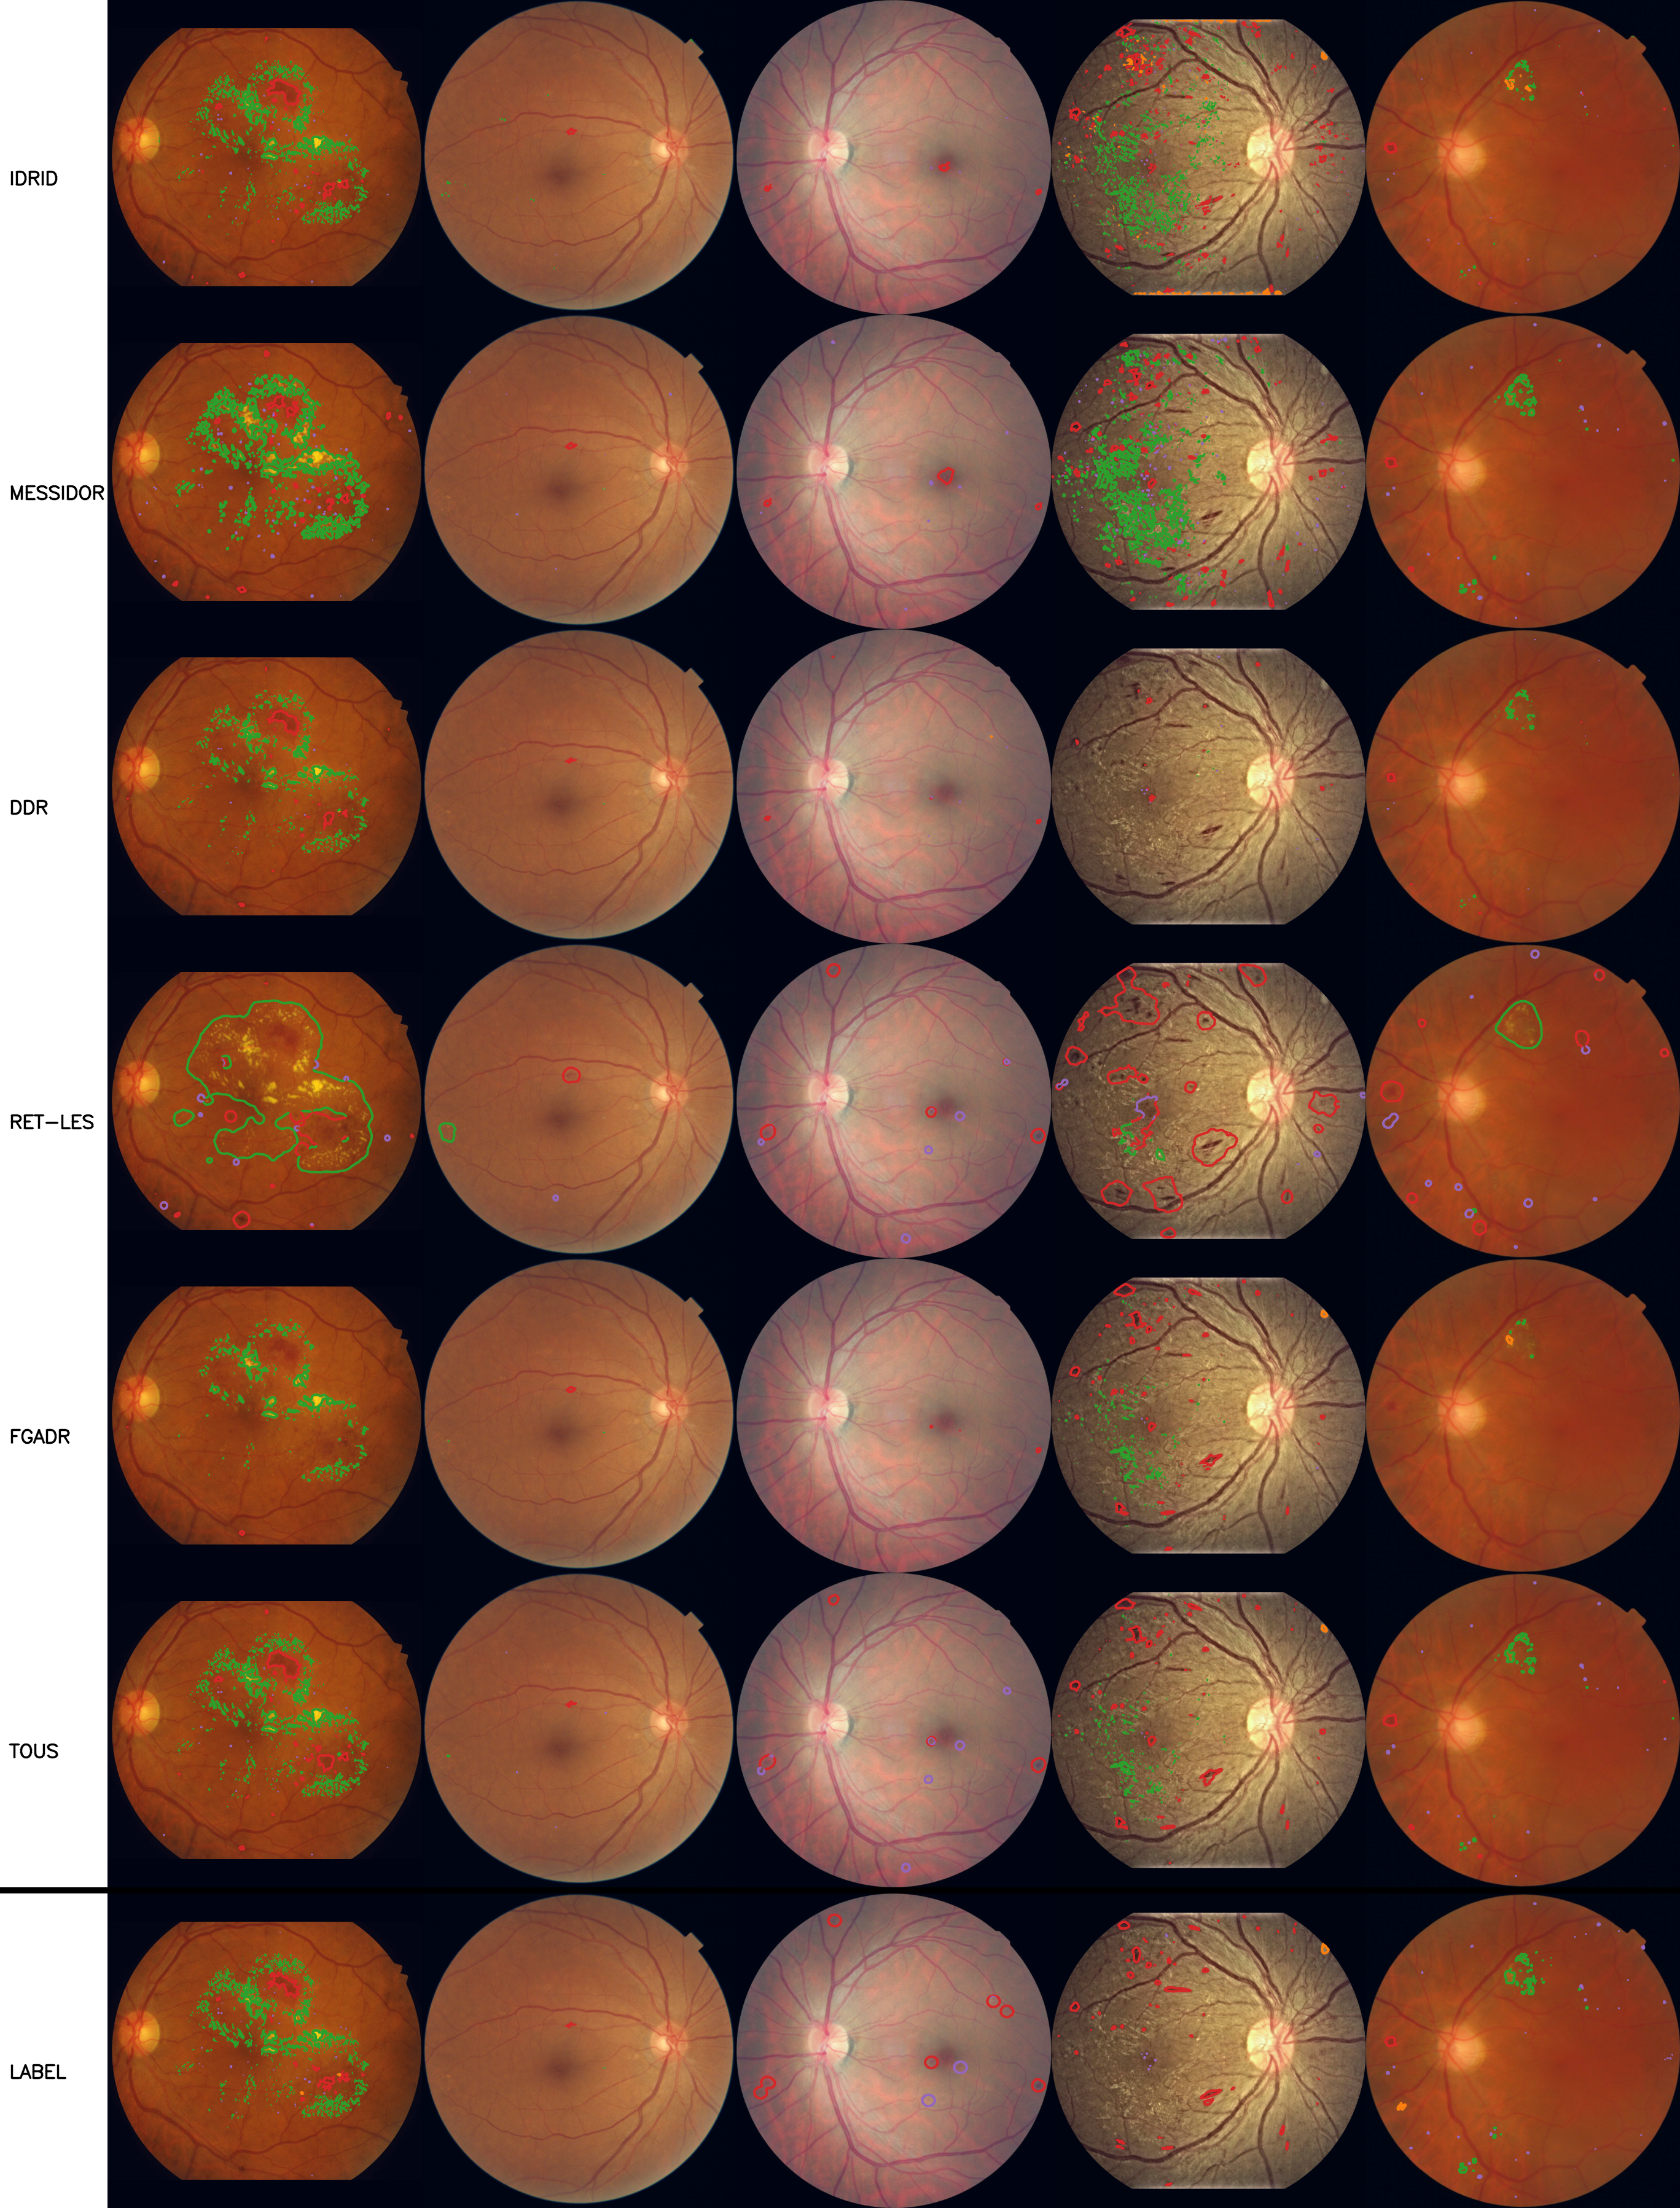
\includegraphics[width=\textwidth]{segmentation_lesions/qualitative_results}
	\caption{Résultats qualitatifs de segmentation inter-bases. Chaque ligne représente un modèle entraîné sur une base. La dernière ligne correspond à la vérité terrain correspondante. Seules les frontières des structures segmentées sont représentées. \textbf{\textcolor{CWScolor}{\ac{CWS}}, \textcolor{EXcolor}{\ac{EX}}, \textcolor{HEcolor}{\ac{HEM}}, \textcolor{MAcolor}{\ac{MA}}}}
	\label{fig:segQualitativeResults}
\end{figure}

\renewcommand{\colSize}{0.26}
\begin{table}
	\caption{Illustration du phénomène du sur-sophistication d'un modèle sur un style d'annotations. Chaque ligne représente un ensemble de test, chaque colonne un modèle. $\mathcal{B}^{(I)}$ représente la base IDRiD, $\mathcal{B}^{(R)}$ la base RET-LES. La dernière colonne illustre le paradoxe du modèle combiné, capable d'adapter son style à la base de test.}
	\label{tab:IllustrationParadoxeModeleCombine}
	\begin{tabular}{m{2cm} ccc}
		\toprule
		& \multicolumn{3}{c}{Modèles} \\
		\midrule
		Bases de test & $\mathcal{M}[\mathcal{B}^{(I)}]$ & $\mathcal{M}[\mathcal{B}^{(R)}]$ &
		$\mathcal{M}[\bigcup_i \mathcal{B}^{(i)}]$ \\
		\midrule
		$\mathcal{B}^{(I)}_{\star}$ (IDRID)& 
		\begin{minipage}{\colSize\textwidth}
			\includegraphics[width=\textwidth]{segmentation_lesions/generalisation/illustration/model_IDRID_images_IDRID.png} 
		\end{minipage} &
		\begin{minipage}{\colSize\textwidth} \includegraphics[width=\textwidth]{segmentation_lesions/generalisation/illustration/model_RETINAL_LESIONS_images_IDRID.png} 
		\end{minipage}& 
		\begin{minipage}{\colSize\textwidth}
			\includegraphics[width=\textwidth]{segmentation_lesions/generalisation/illustration/model_ALL_images_IDRID.png}
		\end{minipage} \\
		\midrule
		$\mathcal{B}^{(R)}_{\star}$ (RET-LES)&
		\begin{minipage}{\colSize\textwidth} \includegraphics[width=\textwidth]{segmentation_lesions/generalisation/illustration/model_IDRID_images_RETINAL_LESIONS.png}
		\end{minipage}&\begin{minipage}{\colSize\textwidth} \includegraphics[width=\textwidth]{segmentation_lesions/generalisation/illustration/model_RETINAL_LESIONS_images_RETINAL_LESIONS.png}
		\end{minipage}&\begin{minipage}{\colSize\textwidth} \includegraphics[width=\textwidth]{segmentation_lesions/generalisation/illustration/model_ALL_images_RETINAL_LESIONS.png}
		\end{minipage}\\
		\bottomrule
	\end{tabular}
\end{table}

\subsection{Adaptation de style par Attaque Adversariable}

\subsubsection{Paradoxe du modèle combiné $\mathcal{M}_{\mathcal{S}}$.}


Les résultats quantitatifs et qualitatifs obtenus des modèles $\mathcal{M}[\mathcal{B}^{(i)}]$ sont attendus: chaque modèle adopte le style d'annotations de sa base d'entraînement et obtient naturellement les meilleures performances sur l'ensemble de test correspondant. La surprise vient en revanche du modèle combiné:  $\mathcal{M}_{\mathcal{S}}$ parvient à surpasser simultanément trois de ces modèles sur leur propre base, ce qui représente un paradoxe apparent considérant que les styles d'annotations de chaque base ne sont pas mutuellement compatibles. On s'attendait alors à ce que le modèle adopte le style dominant (ou un style qui représente le meilleur compromis entre chaque base). L'observation des segmentations produites par $\mathcal{M}_{\mathcal{S}}$ résout ce paradoxe (voir le tableau \ref{tab:IllustrationParadoxeModeleCombine}) non sans soulever d'autres questions: on y voit que le modèle combiné est capable d'ajuster son style de segmentation en fonction de la base d'origine de l'image. Précisons bien qu'il s'agit d'images qui n'ont pas servi à l'entraînement du modèle, donc bien issues de l'ensemble d'évaluation. Le réseau n'a donc a priori pas d'informations sur le style d'annotations attendu, mais il arrive pourtant à identifier la base d'origine de l'image, et à adapter sa segmentation à un style concordant. Cette capacité lui permet donc d'obtenir des performances maximales sur les distributions distinctes de chaque base. Elle n'en reste pas moins surprenante: le modèle ne prend pour entrée qu'une image et n'a donc pas accès à son origine de manière explicite. L'unique explication est qu'il existe au sein d'une image un marqueur permettant d'identifier sa base d'appartenance. Le modèle $\mathcal{M}_{\mathcal{S}}$ apprend à reconnaître ce marqueur, à le lire à l'inférence et modifier sa sortie en fonction. Et bien qu'innattendu, cet effet peut s'expliquer: les différentes bases contiennent en leur sein des images dont l'intra-variabilité est plus faible que l'inter-variabilité entre bases. En effet,  au sein d'une même base, les images sont acquises dans des conditions relativement homogènes: c'est-à-dire même matériel d'acquisition et résolution d'acquisition. Par ailleurs, on peut aussi supposer d'une ethnicité relativement homogène au sein de la population représentée dans chaque base. L'hypothèse d'un marqueur de base identifiable dans chaque image n'est donc pas invraisemblable. 
\\
Mais une fois ce comportement de $\mathcal{M}_\mathcal{S}$ identifié, plusieurs questions se posent:
\begin{itemize}
	\item Est-il possible d'identifier le marqueur implicite contenu dans l'image qui trahit son origine?
	\item Comment le modèle de segmentation lit-il ce marqueur pour ajuster sa prédiction?
	\item Finalement, peut-on contraindre de manière prédictible le style de segmentation du modèle en manipulant ce marqueur de base?
\end{itemize}

Précisons que par la suite, nous prendrons souvent IDRiD et RET-LES en exemple car ces deux bases sont les plus radicalement différentes dans leur style d'annotations respectif.
\subsubsection{Robustesse de l'identification de base}
De manière préliminaire, nous avons voulu tester la sensibilité de la phase d'identification du marqueur lorsqu'on soumet l'image fournie au modèle à diverses perturbations simples. Pour nos expériences, celles-ci sont de deux types: géométriques ou colorimétriques. Dans le premier cas, on sous-échantillonne l'image (par un facteur 4) avant de la redimensionner à son échelle originale. Cette opération est équivalente à l'application d'un filtre passe-bas et simule une résolution d'acquisition variable. Elle vise à vérifier que le marqueur d'appartenance à une base n'est pas liée à une certaine composante haute fréquence imperceptible présente dans l'image. La seconde opération modifie de manière aléatoire la teinte, la saturation, la luminosité et le contraste de l'image (dans la limite de 20\% d'altérations). Enfin, pour évaluer si la distinction entre base ne provient pas de la compression choisie des images, nous étudions l'effet de celle-ci dans un scénario exacerbé (réduction par compression JPEG à 40\% du poids en octet de l'image originale). Comme en témoignent les résultats sur le tableau \ref{tab:PerturbationsIdentificationsMarqueursDB}, aucune de ces approches ne perturbe le style de segmentation choisi par le réseau de manière probante, à l'exception dans une moindre mesure de la compression JPEG.

\renewcommand{\colSize}{0.3}
\begin{table}
	\centering
	\caption{Pour identifier le marqueur de base de données dans l'image, des perturbations géométriques ou colorimétriques sont appliquées à celle-ci. Ces perturbations n'ont pas d'effet sur le style de segmentation choisi par le modèle. Marginalement, le niveau de compression peut avoir un léger effet sur $\mathcal{B}^{(I)}_{\star}$.}
	\label{tab:PerturbationsIdentificationsMarqueursDB}
	\begin{tabular}{m{5cm} cc}
		\toprule
		Modèles & \multicolumn{2}{|c}{Bases} \\
		\midrule
		 & $\mathcal{B}^{(I)}_{\star}$ (IDRID)& $\mathcal{B}^{(R)}_{\star}$ (RET-LES)\\
		\midrule
		$\mathcal{M}[\bigcup_i \mathcal{B}^{(i)}]$ (Référence) & 
		\begin{minipage}{\colSize\textwidth}
		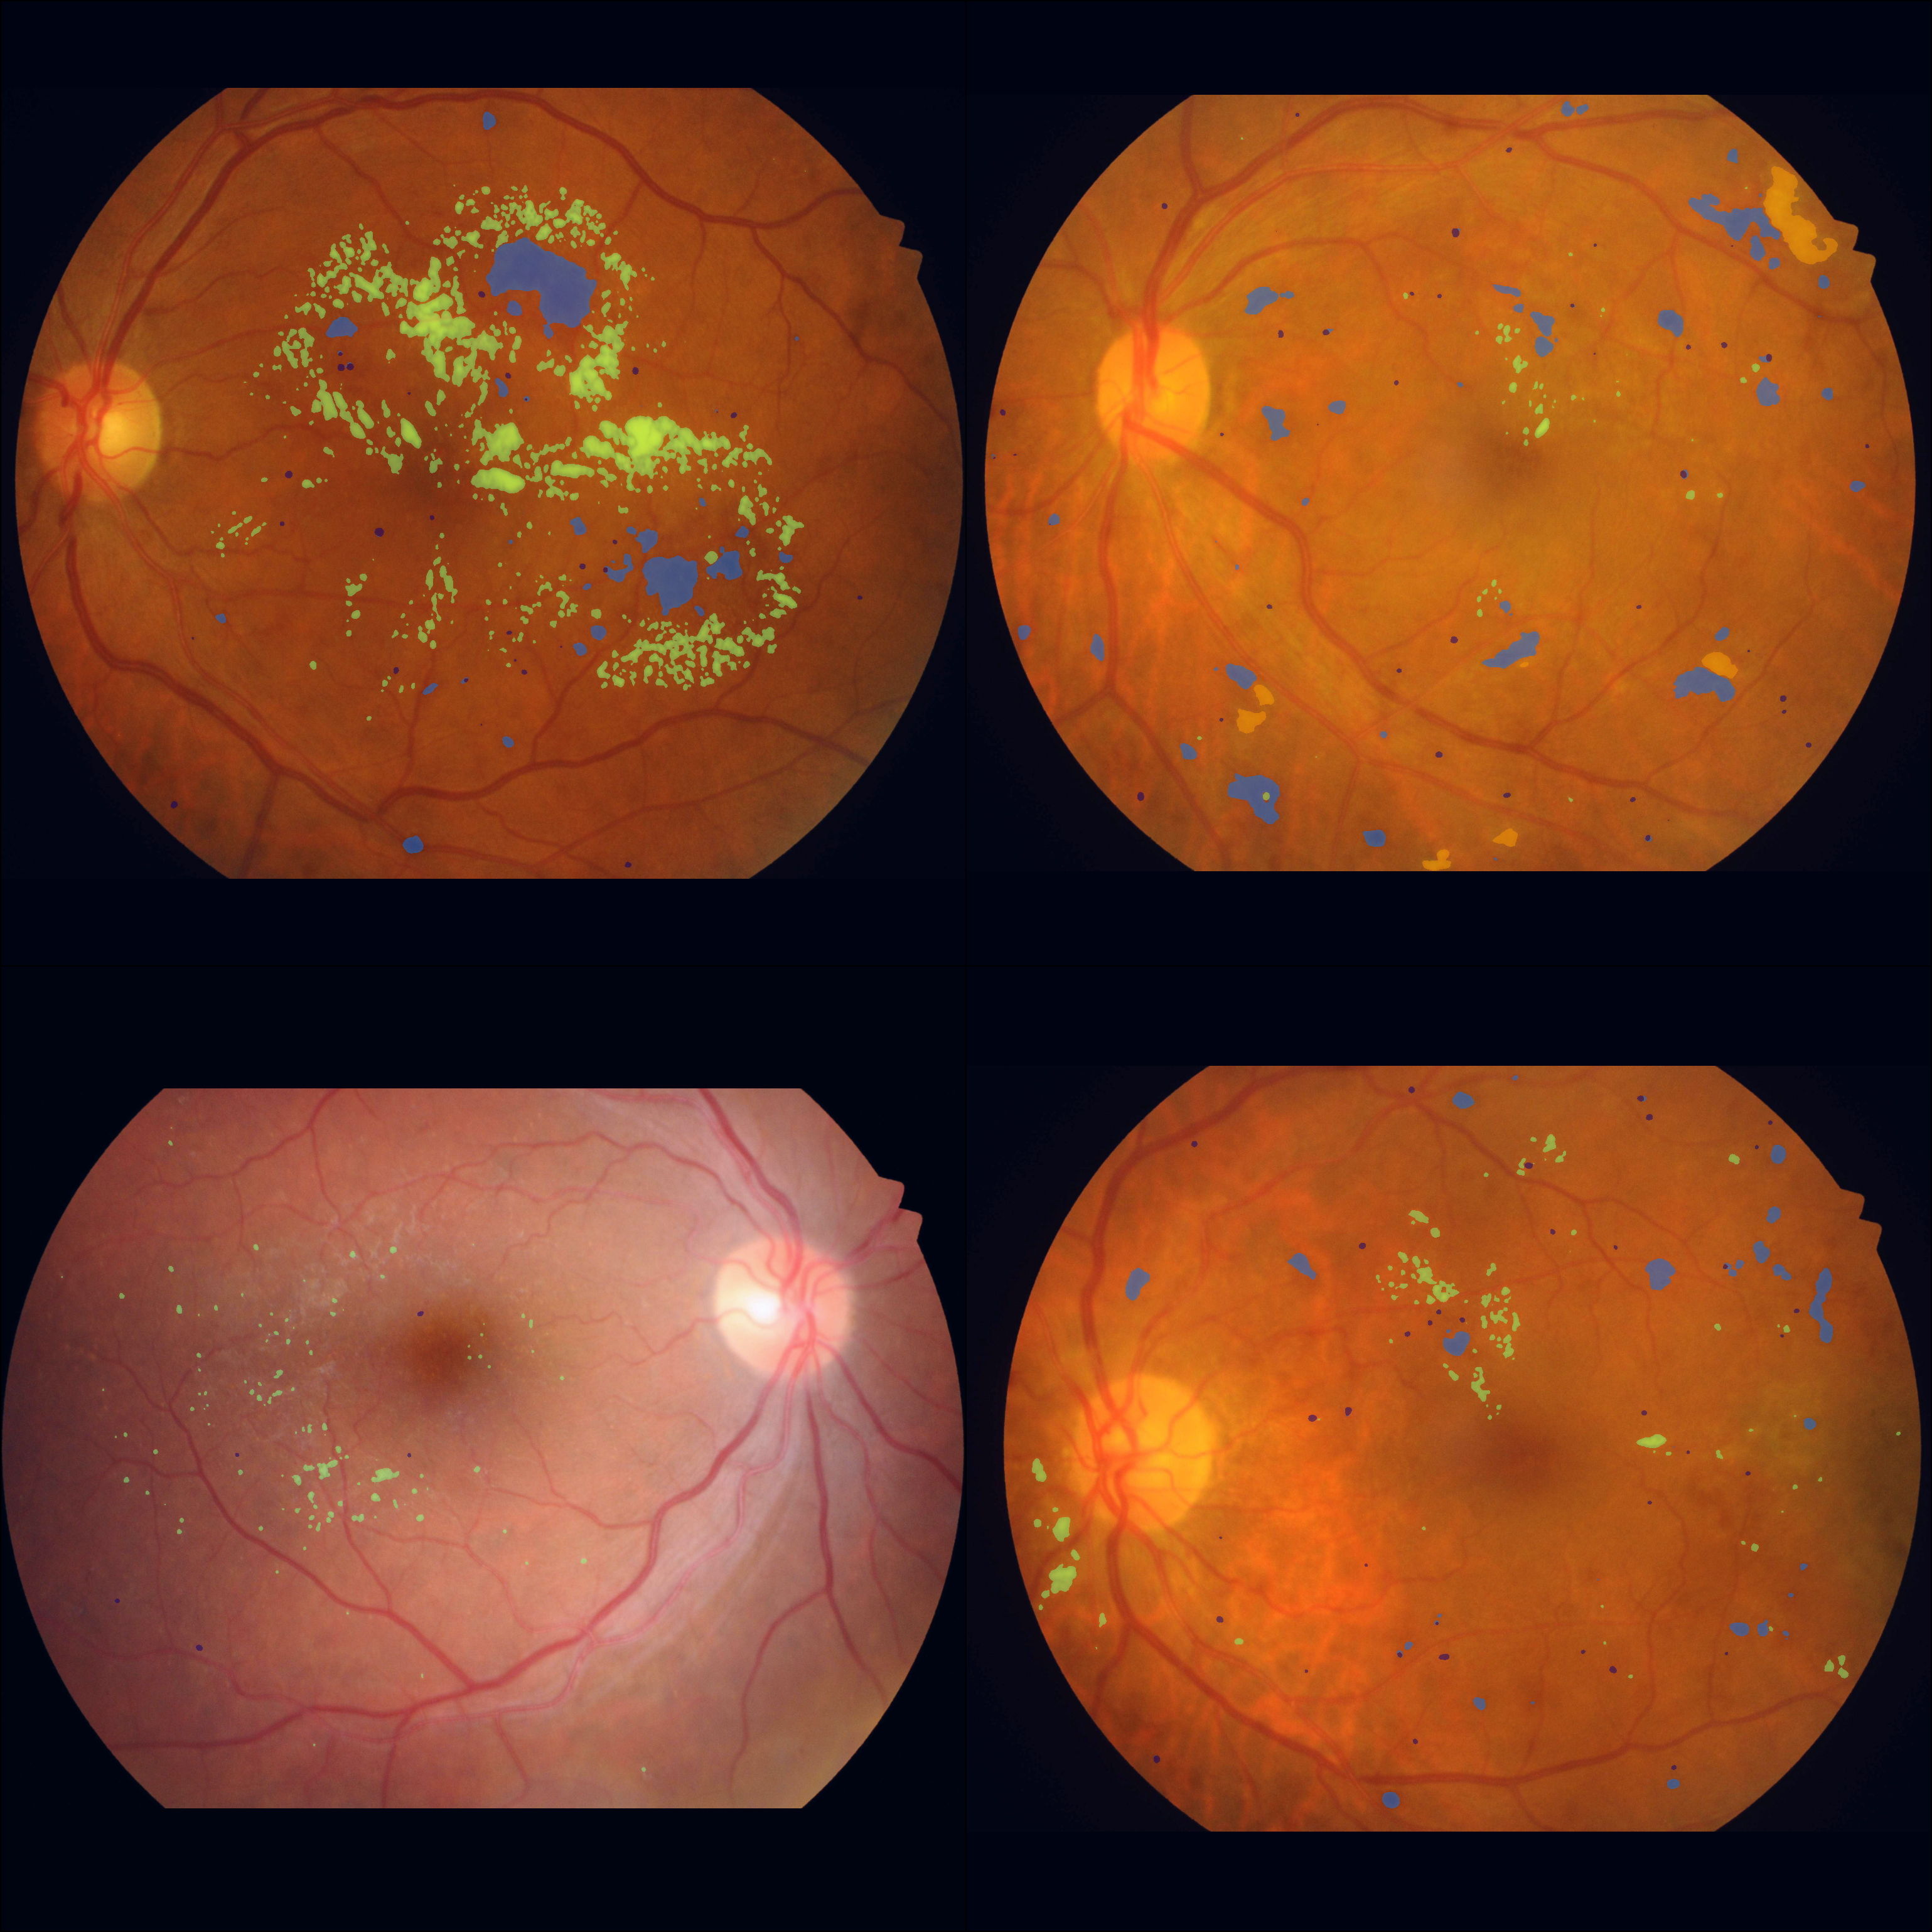
\includegraphics[width=\textwidth]{segmentation_lesions/generalisation/CombinedModelTricking/model_ALL_images_IDRID_ref}
		\end{minipage}
	& 
	\begin{minipage}{\colSize\textwidth}
		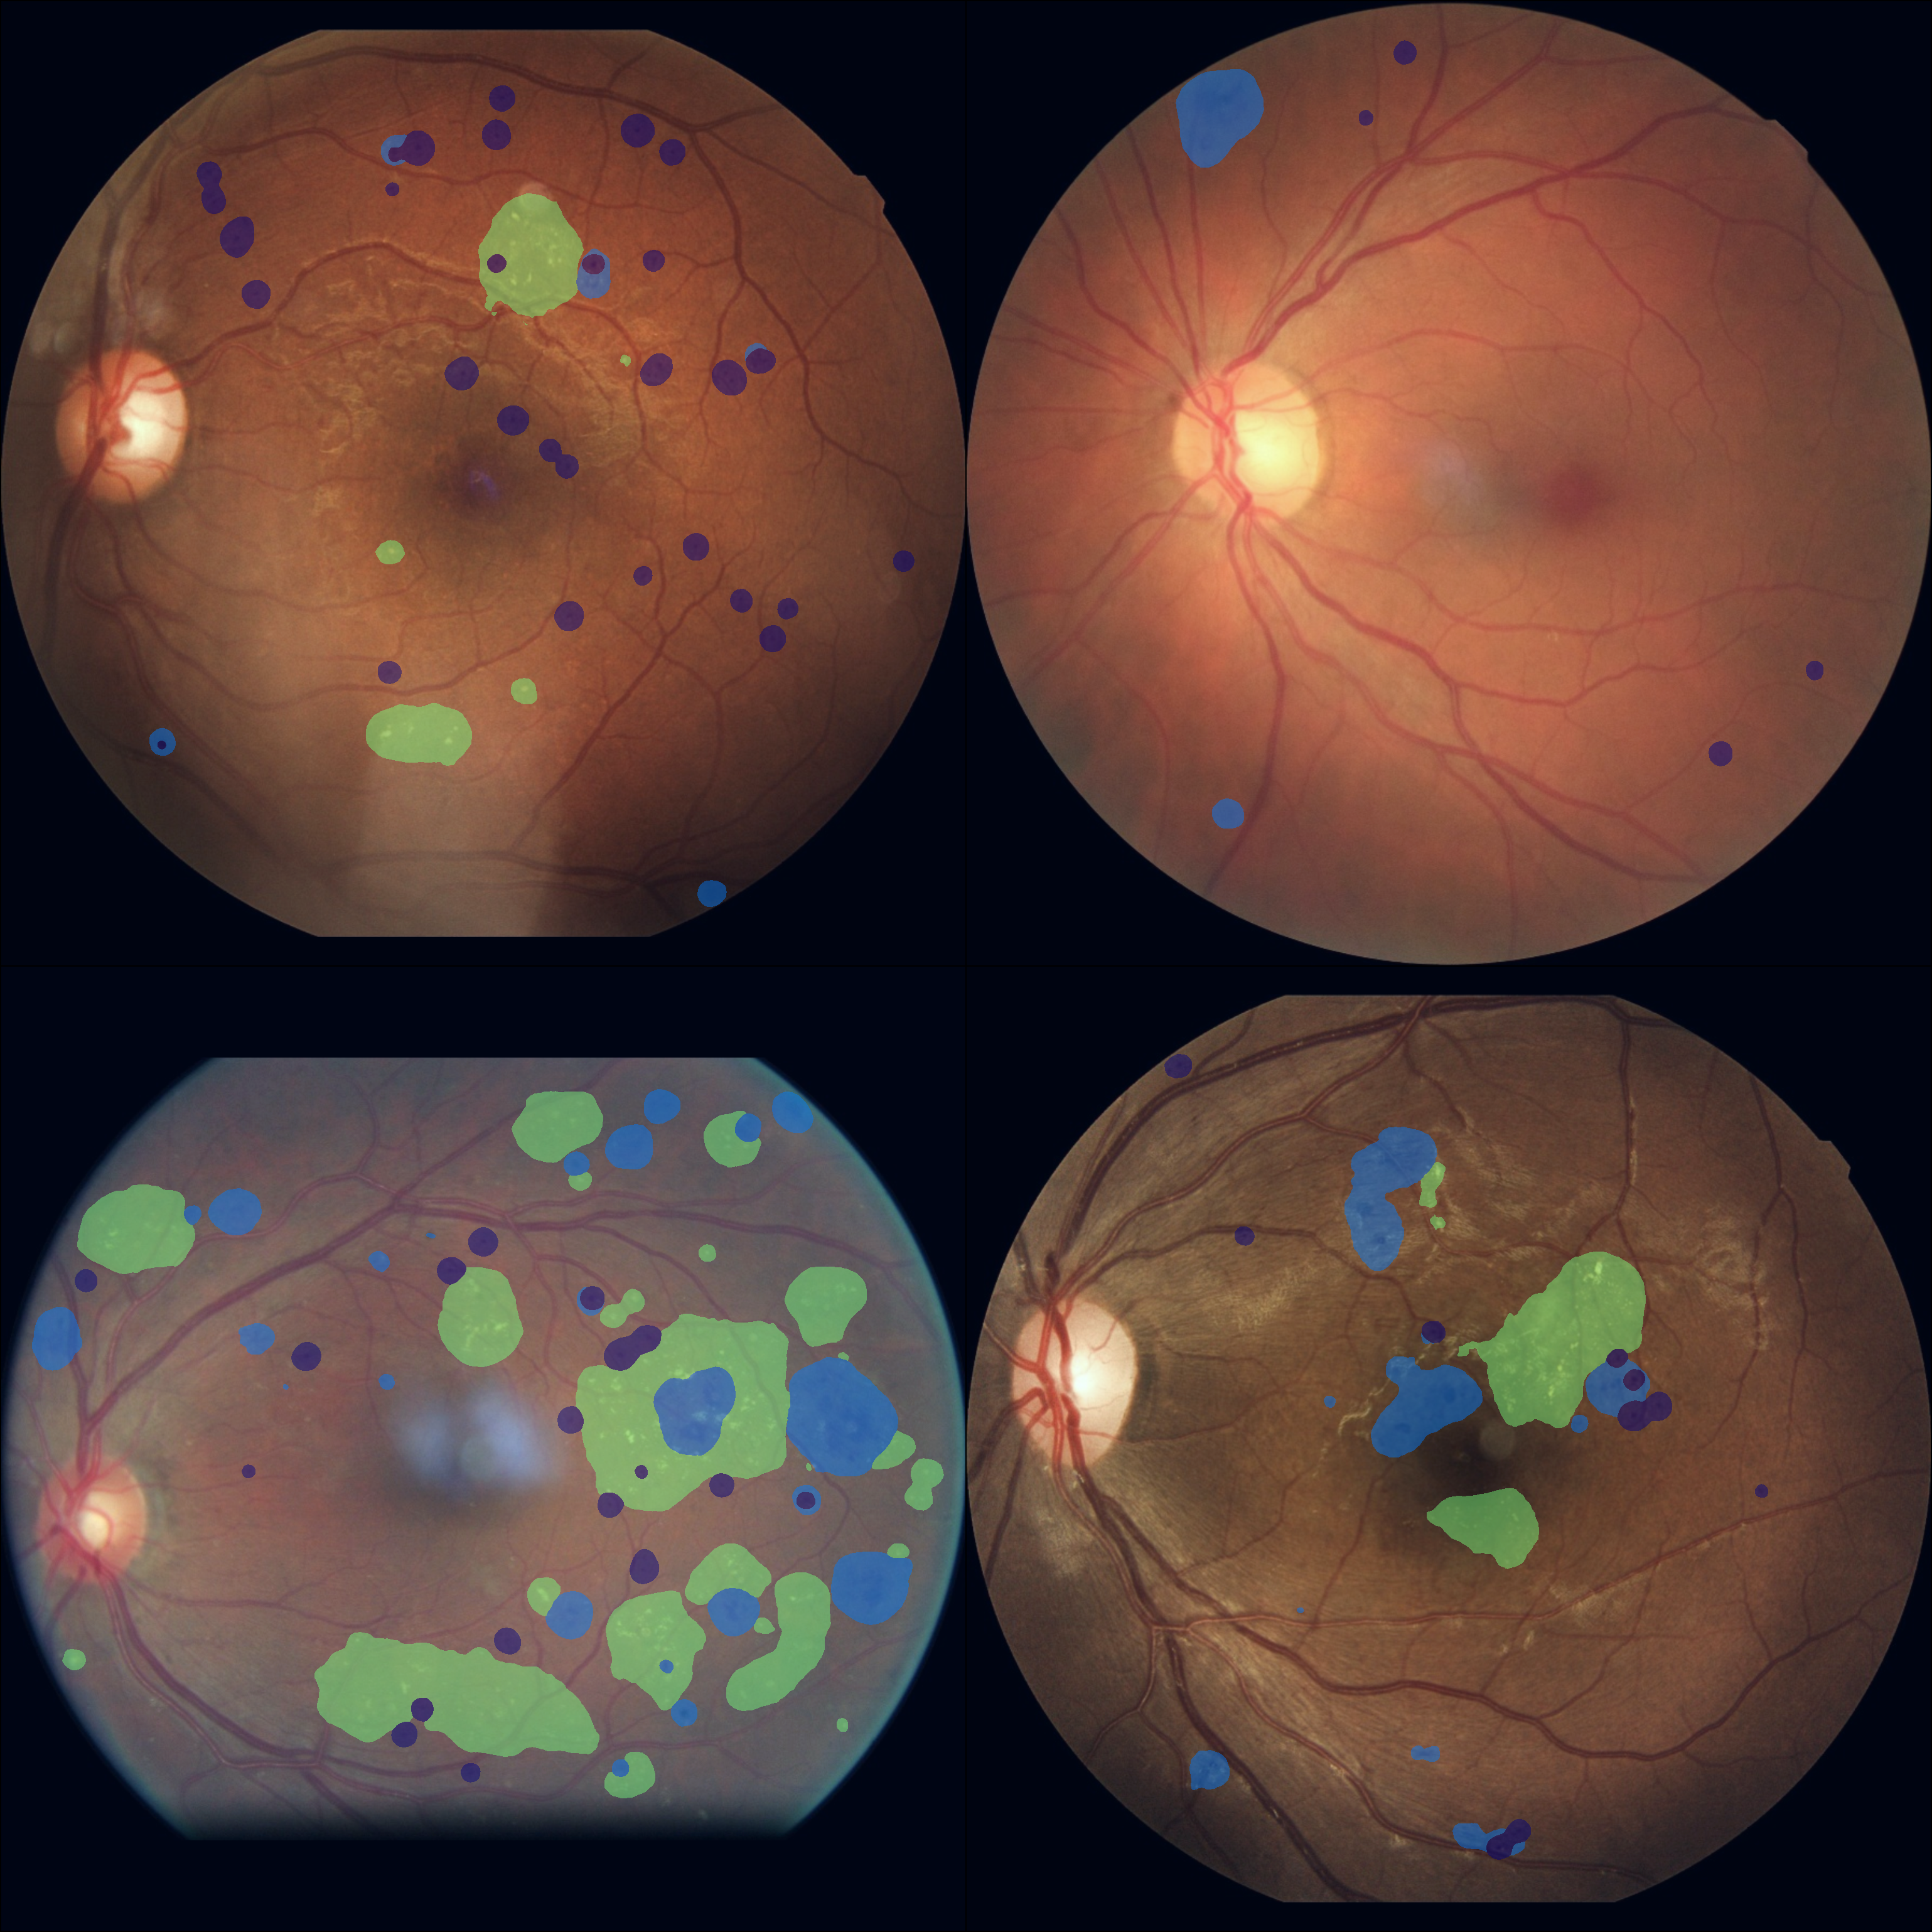
\includegraphics[width=\textwidth]{segmentation_lesions/generalisation/CombinedModelTricking/model_ALL_images_RETINAL_LESIONS_ref}
	\end{minipage}
	\\
	\midrule
	\midrule
	$\mathcal{M}[\bigcup_i \mathcal{B}^{(i)}]$ + 
	Variation d'échelle (résolution $\times 25\%$) & \begin{minipage}{\colSize\textwidth}
		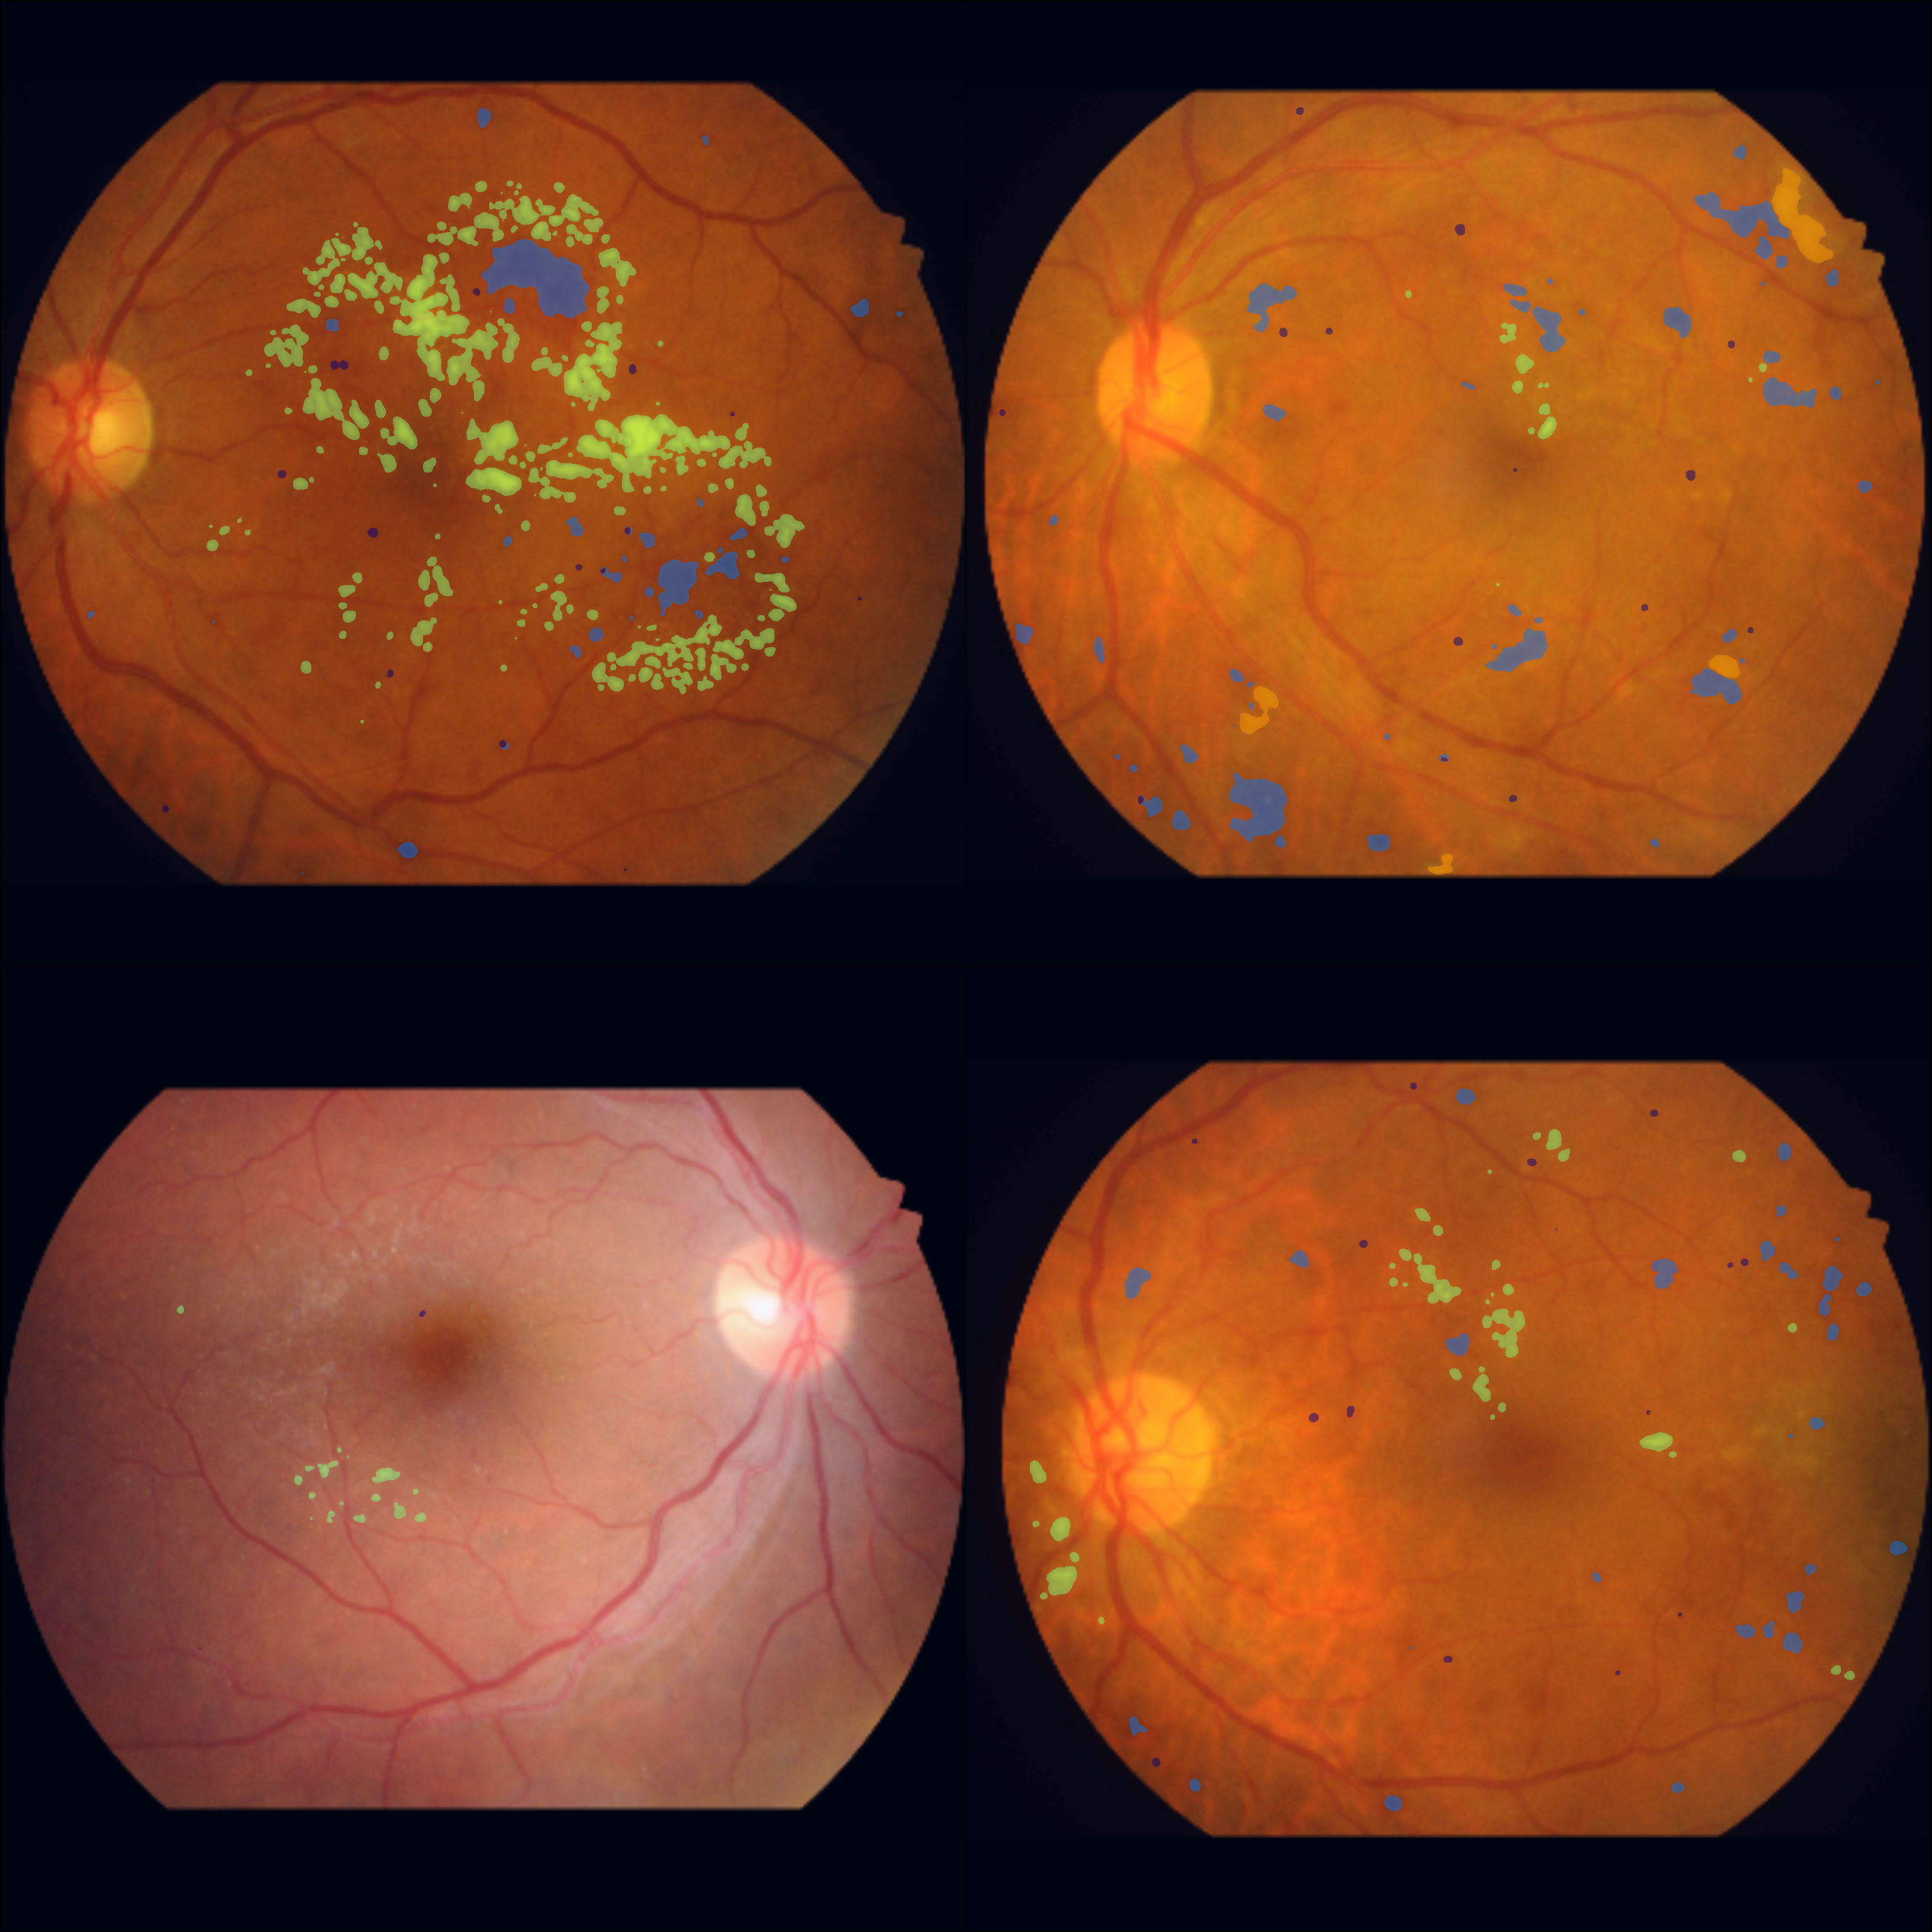
\includegraphics[width=\textwidth]{segmentation_lesions/generalisation/CombinedModelTricking/model_ALL_images_IDRID_randomResize}
	\end{minipage}
	& 
	\begin{minipage}{\colSize\textwidth}
		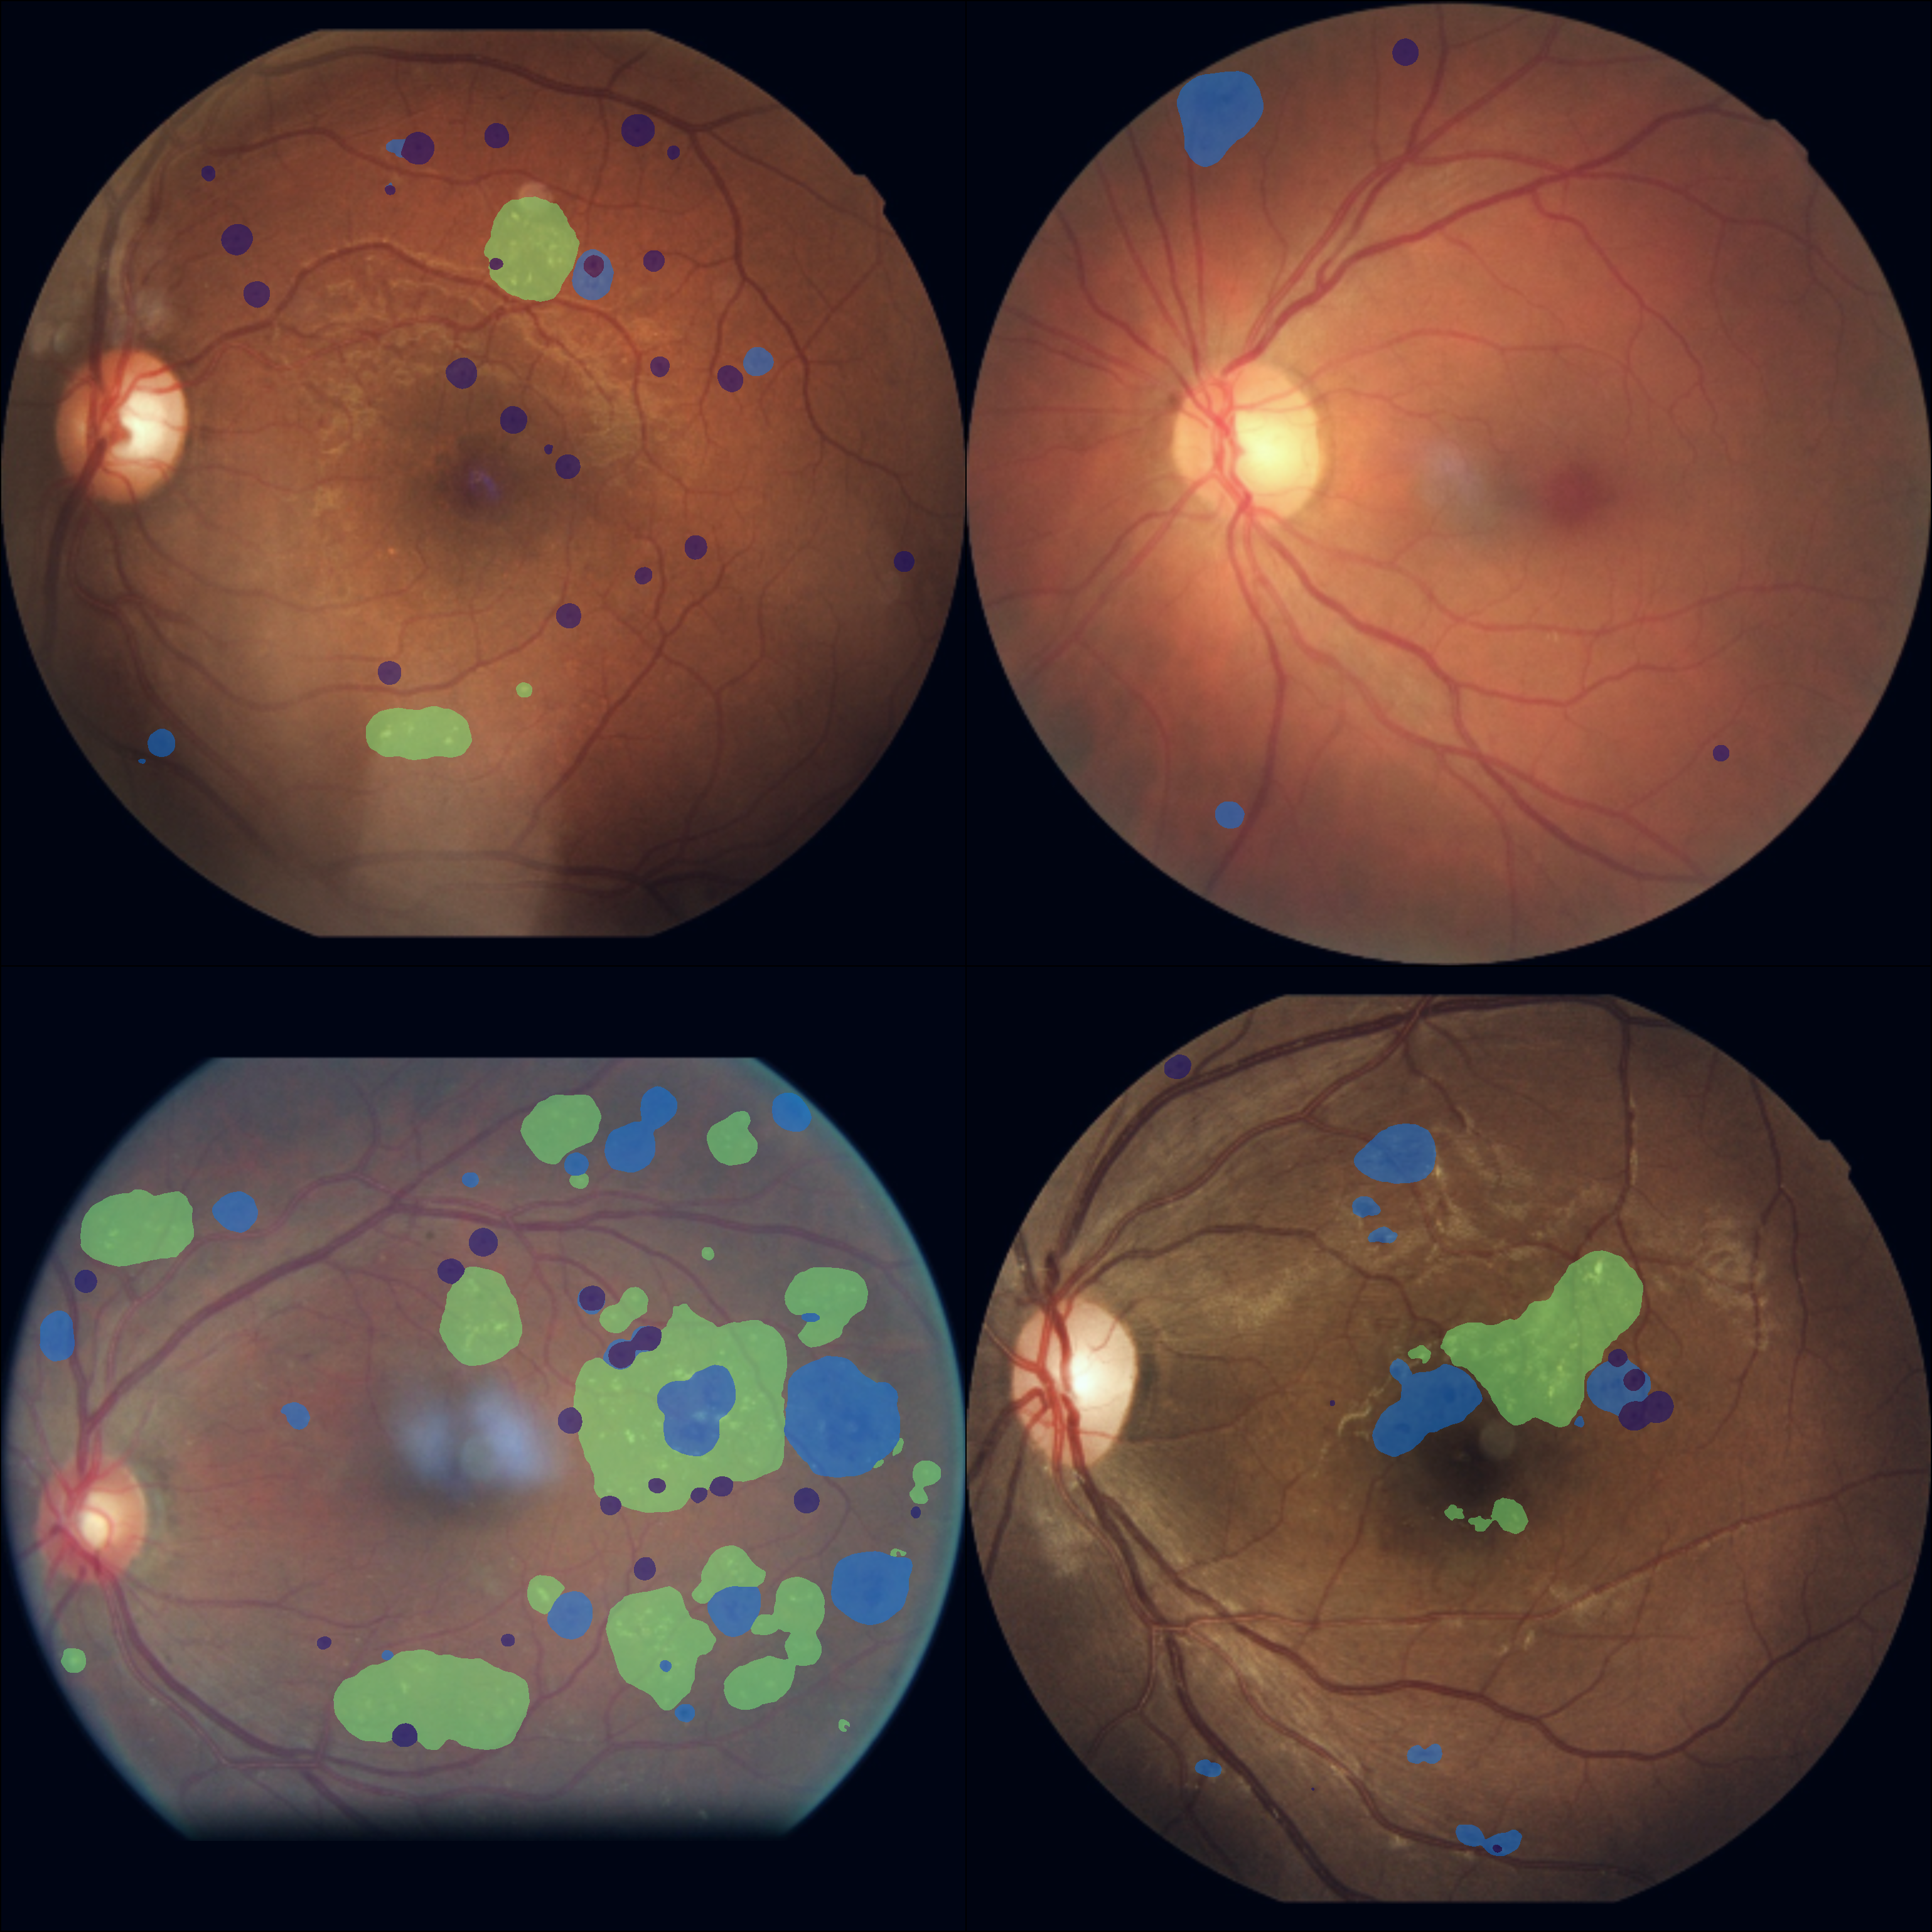
\includegraphics[width=\textwidth]{segmentation_lesions/generalisation/CombinedModelTricking/model_ALL_images_RETINAL_LESIONS_randomResize}
	\end{minipage} \\
\midrule
$\mathcal{M}[\bigcup_i \mathcal{B}^{(i)}]$ +
		Variation colorimétrique (saturation, teinte, contraste, luminosité) & \begin{minipage}{\colSize\textwidth}
			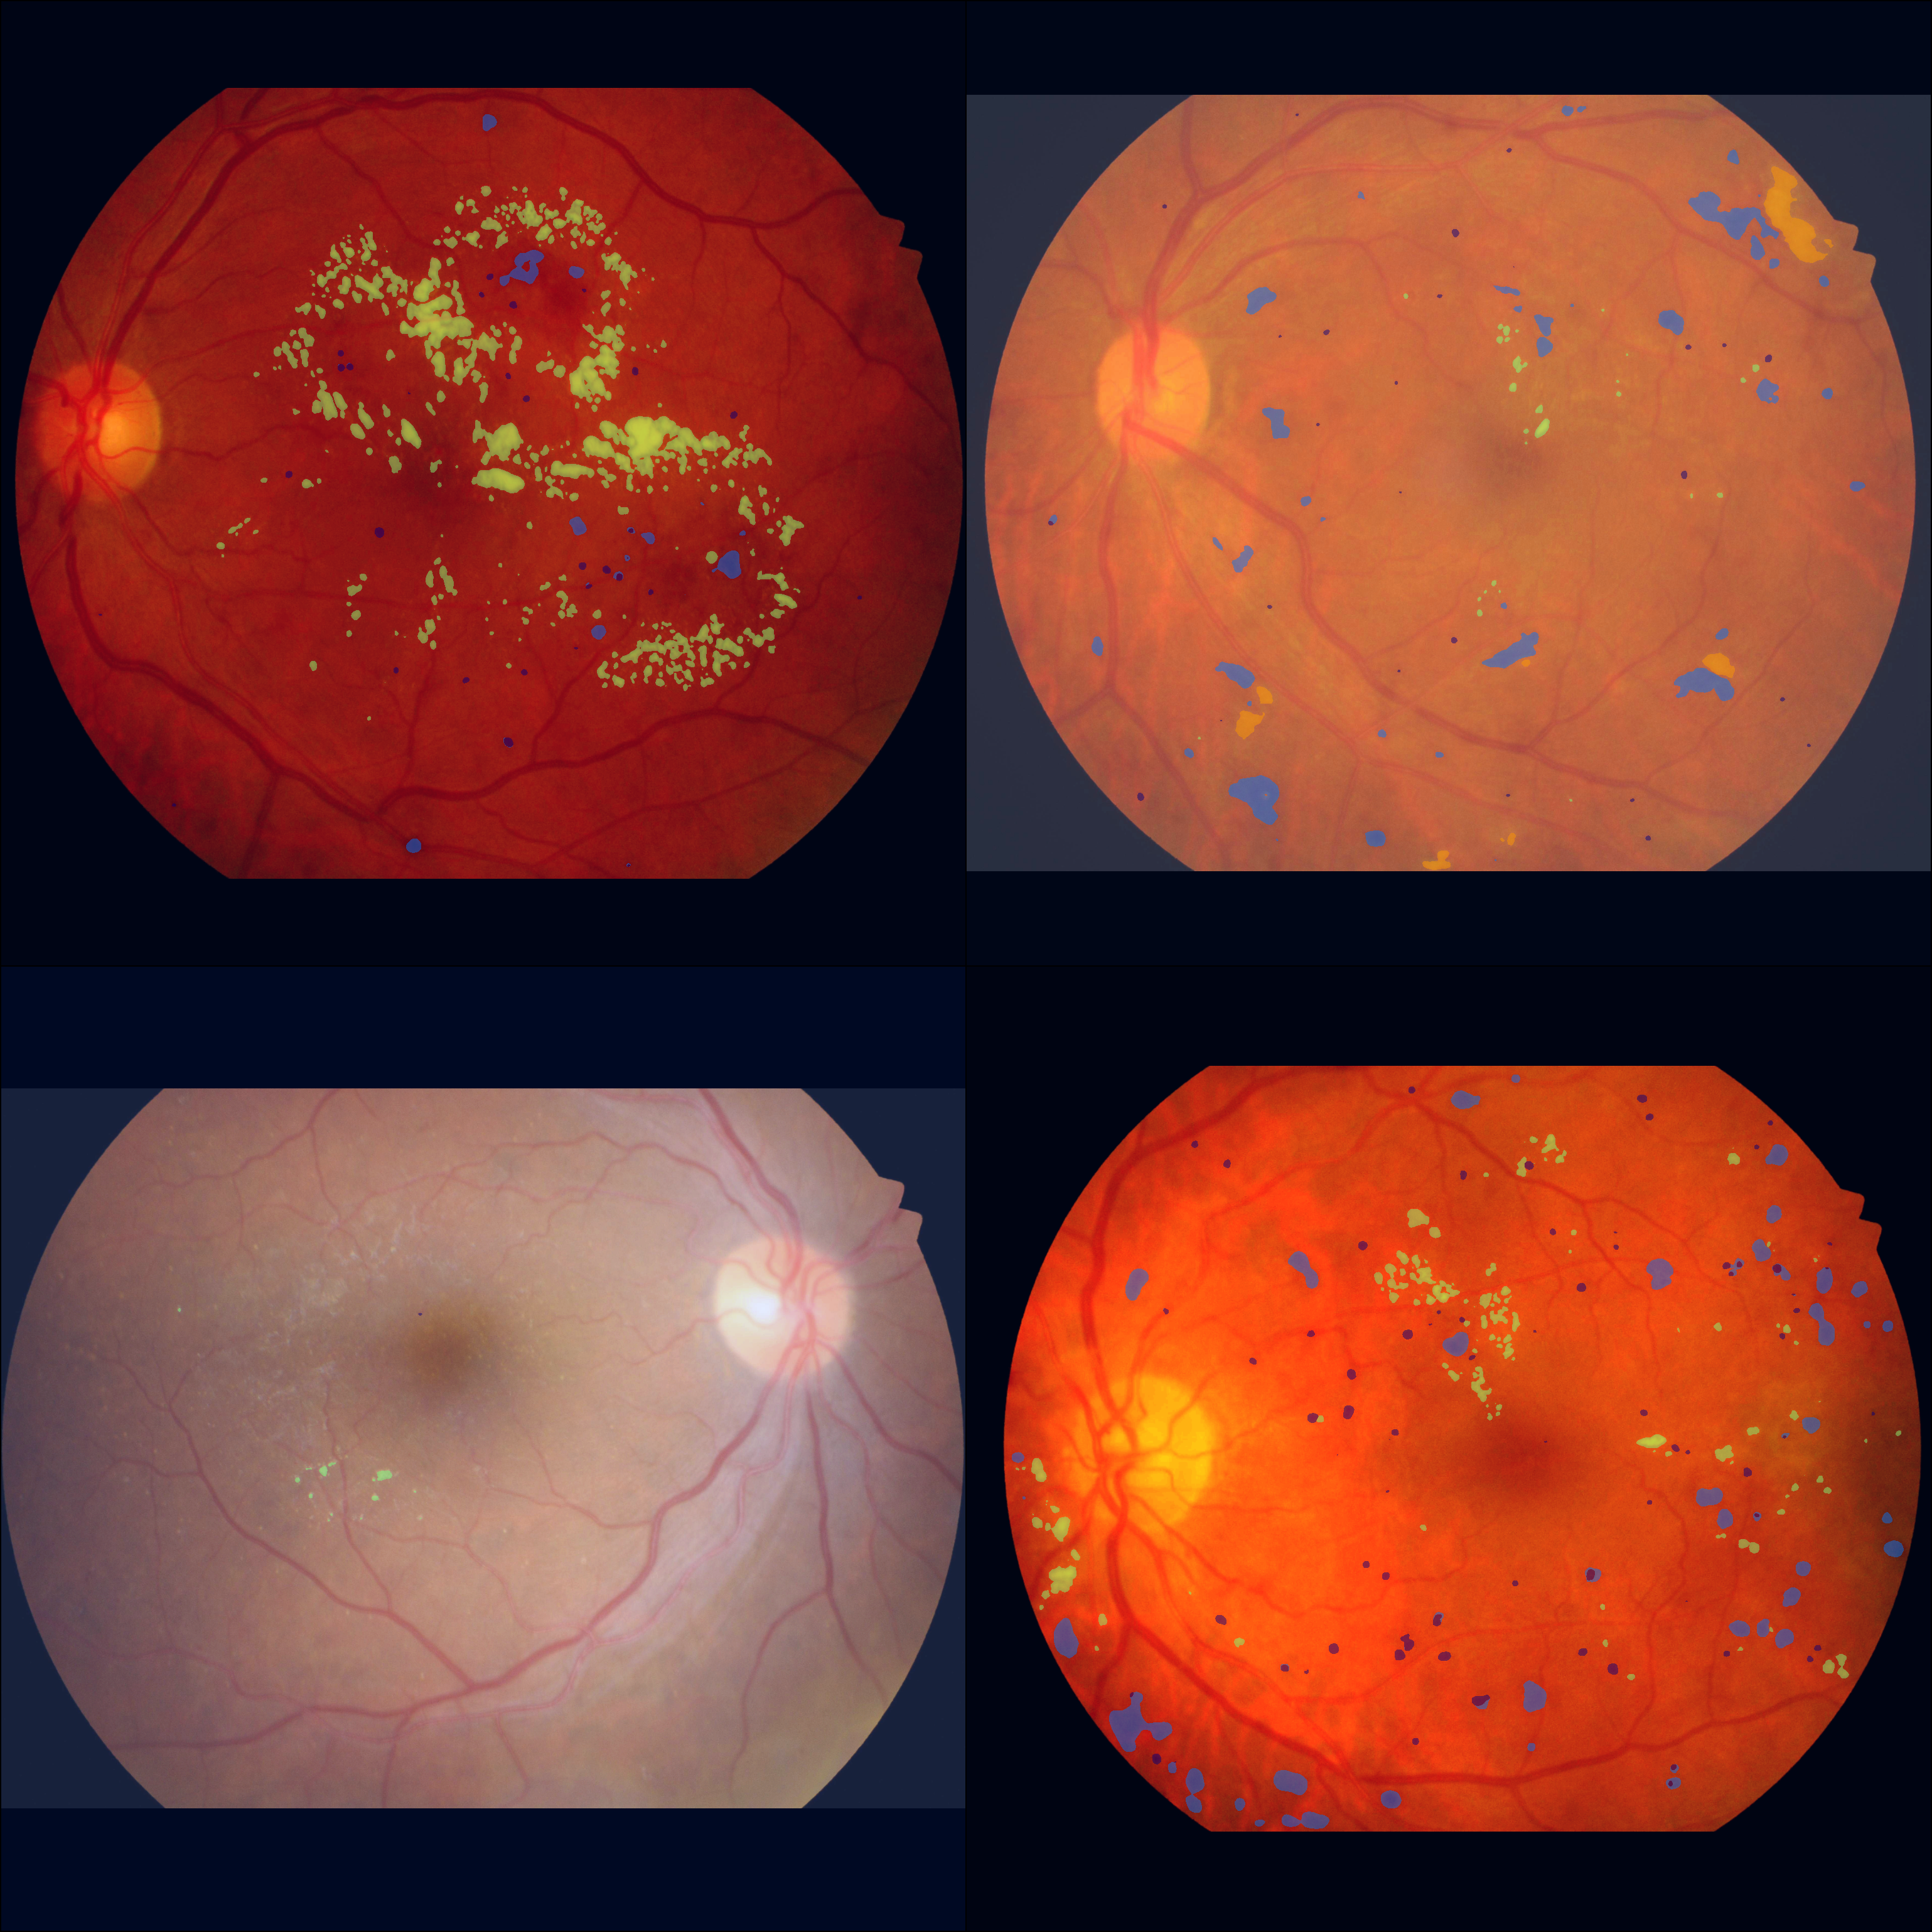
\includegraphics[width=\textwidth]{segmentation_lesions/generalisation/CombinedModelTricking/model_ALL_images_IDRID_colorJitter}
		\end{minipage}
		& 
		\begin{minipage}{\colSize\textwidth}
			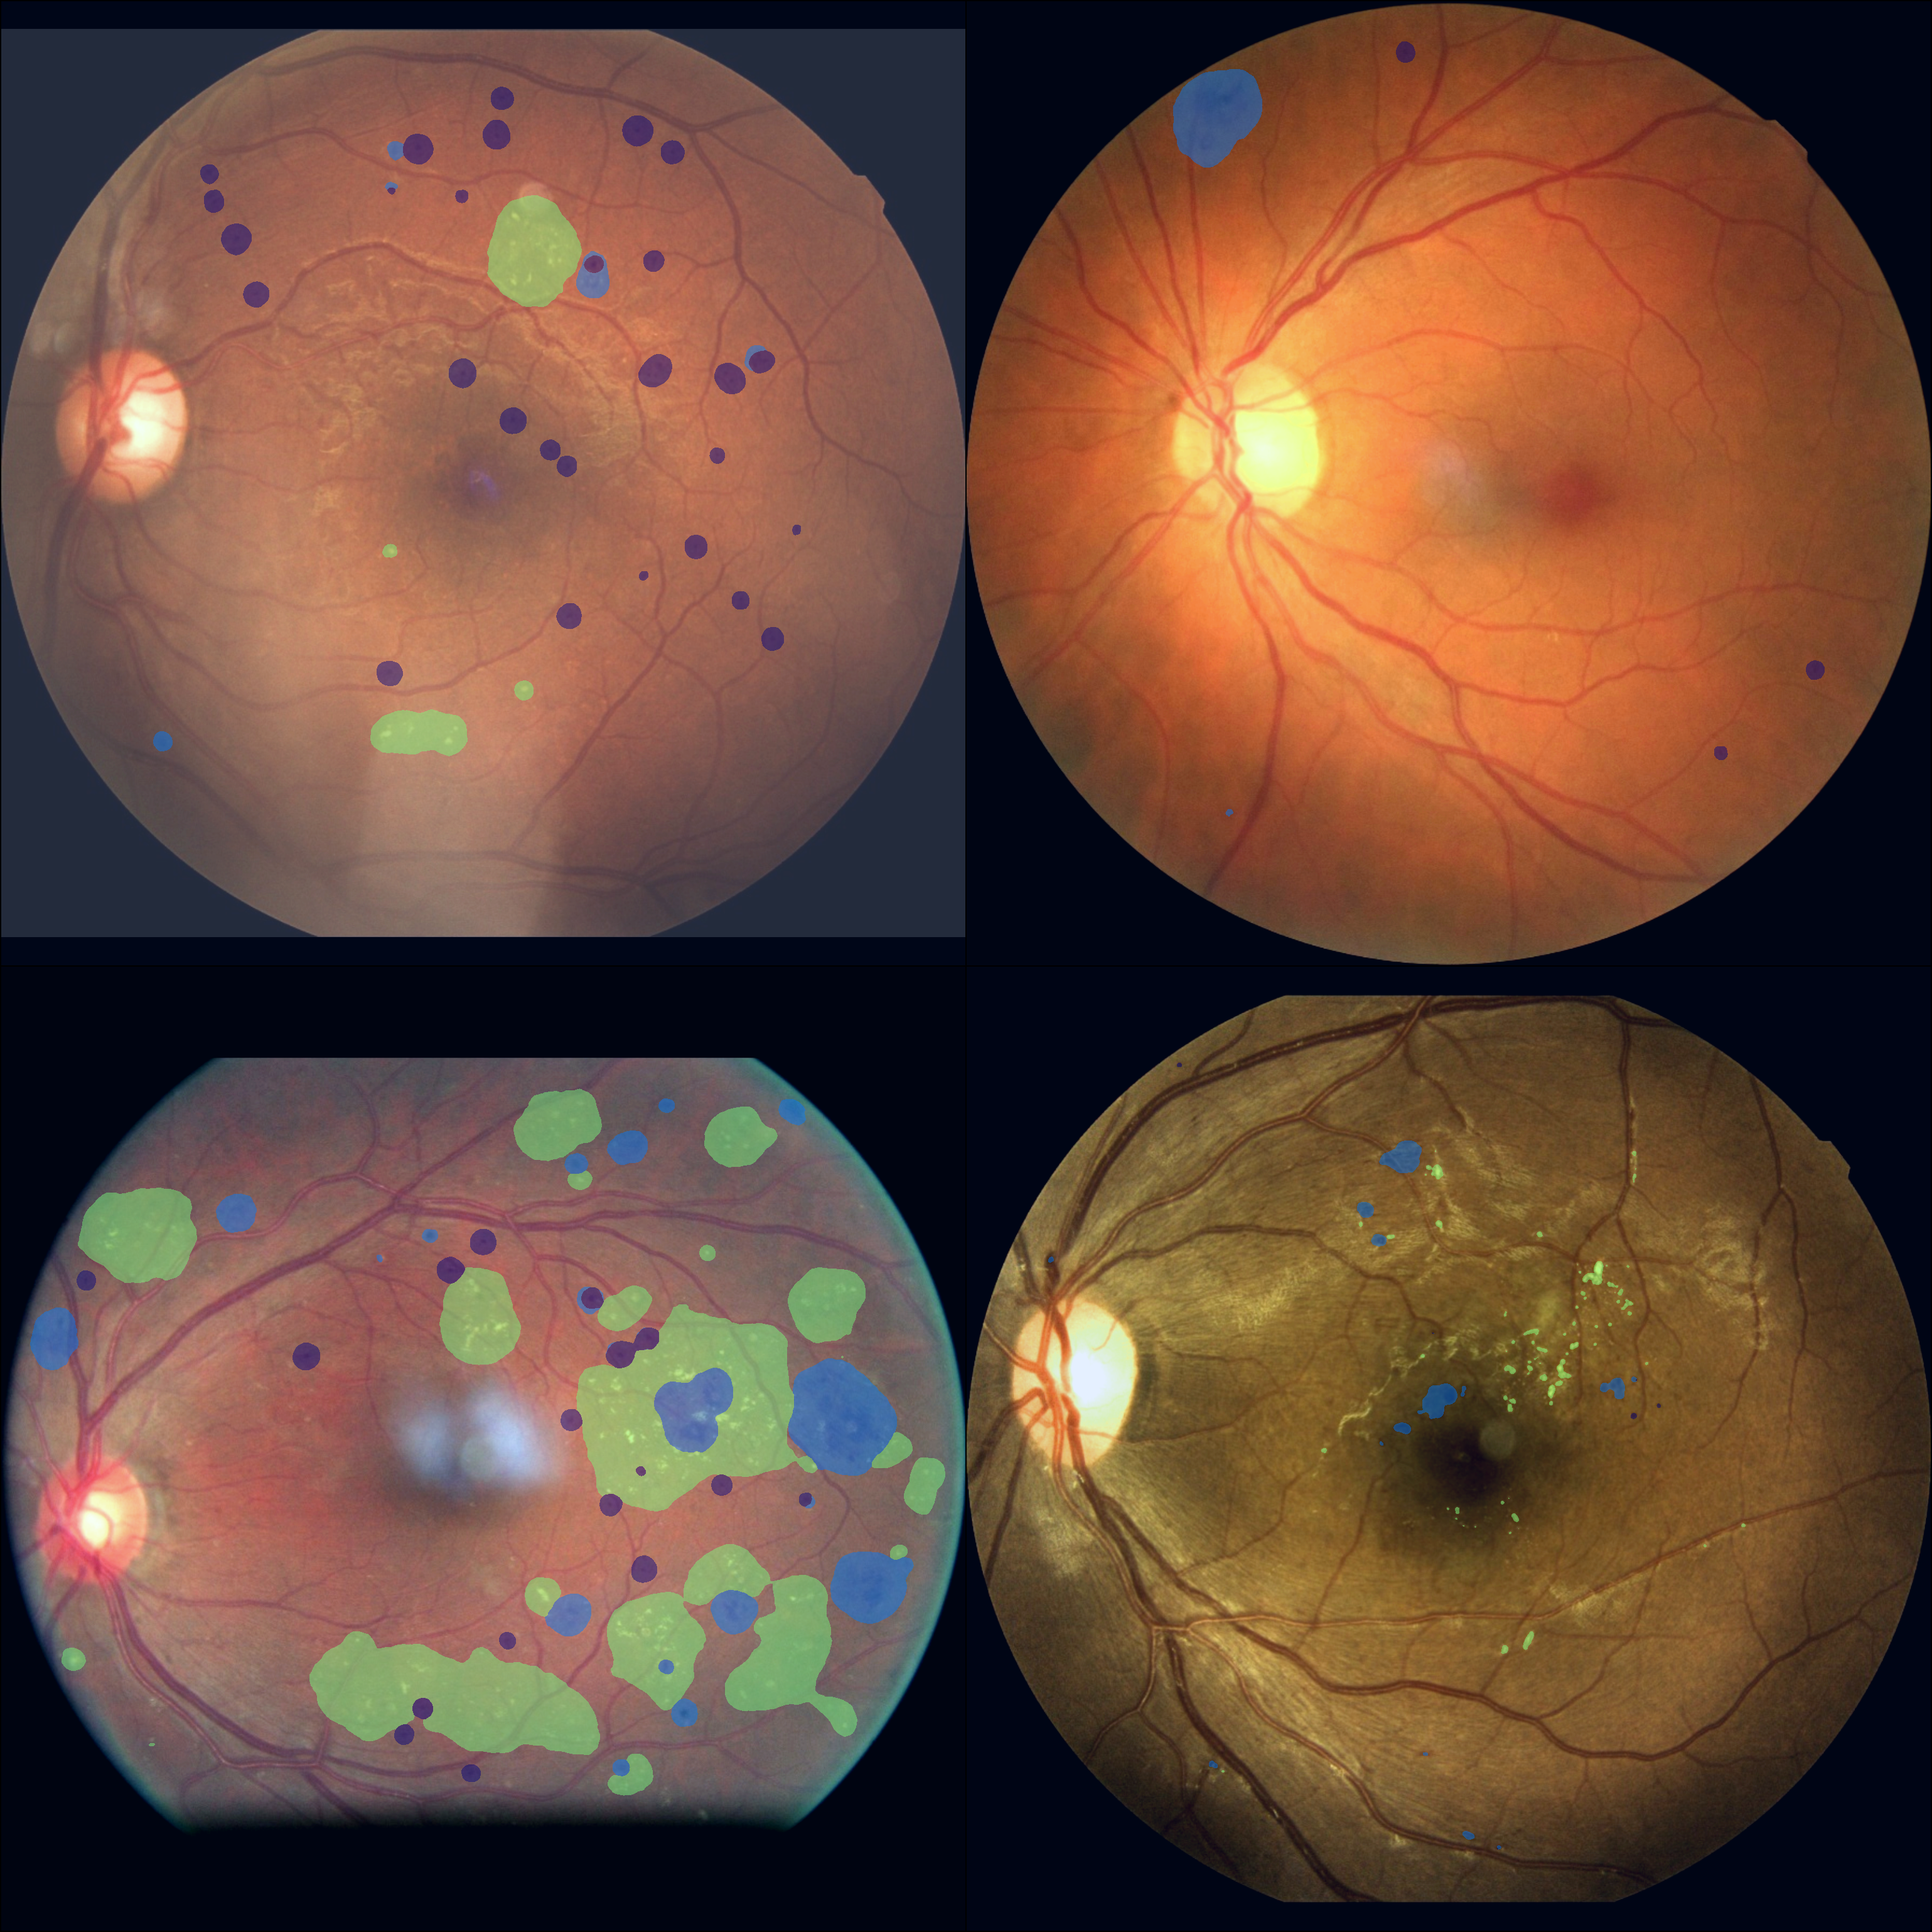
\includegraphics[width=\textwidth]{segmentation_lesions/generalisation/CombinedModelTricking/model_ALL_images_RETINAL_LESIONS_colorJitter}
		\end{minipage} \\
	\midrule
	$\mathcal{M}[\bigcup_i \mathcal{B}^{(i)}]$ + 
	Compression JPEG (40\%) 
	& \begin{minipage}{\colSize\textwidth}
		\includegraphics[width=\textwidth]{segmentation_lesions/generalisation/CombinedModelTricking/model_ALL_images_IDRID_compression}
	\end{minipage}
	& 
	\begin{minipage}{\colSize\textwidth}
		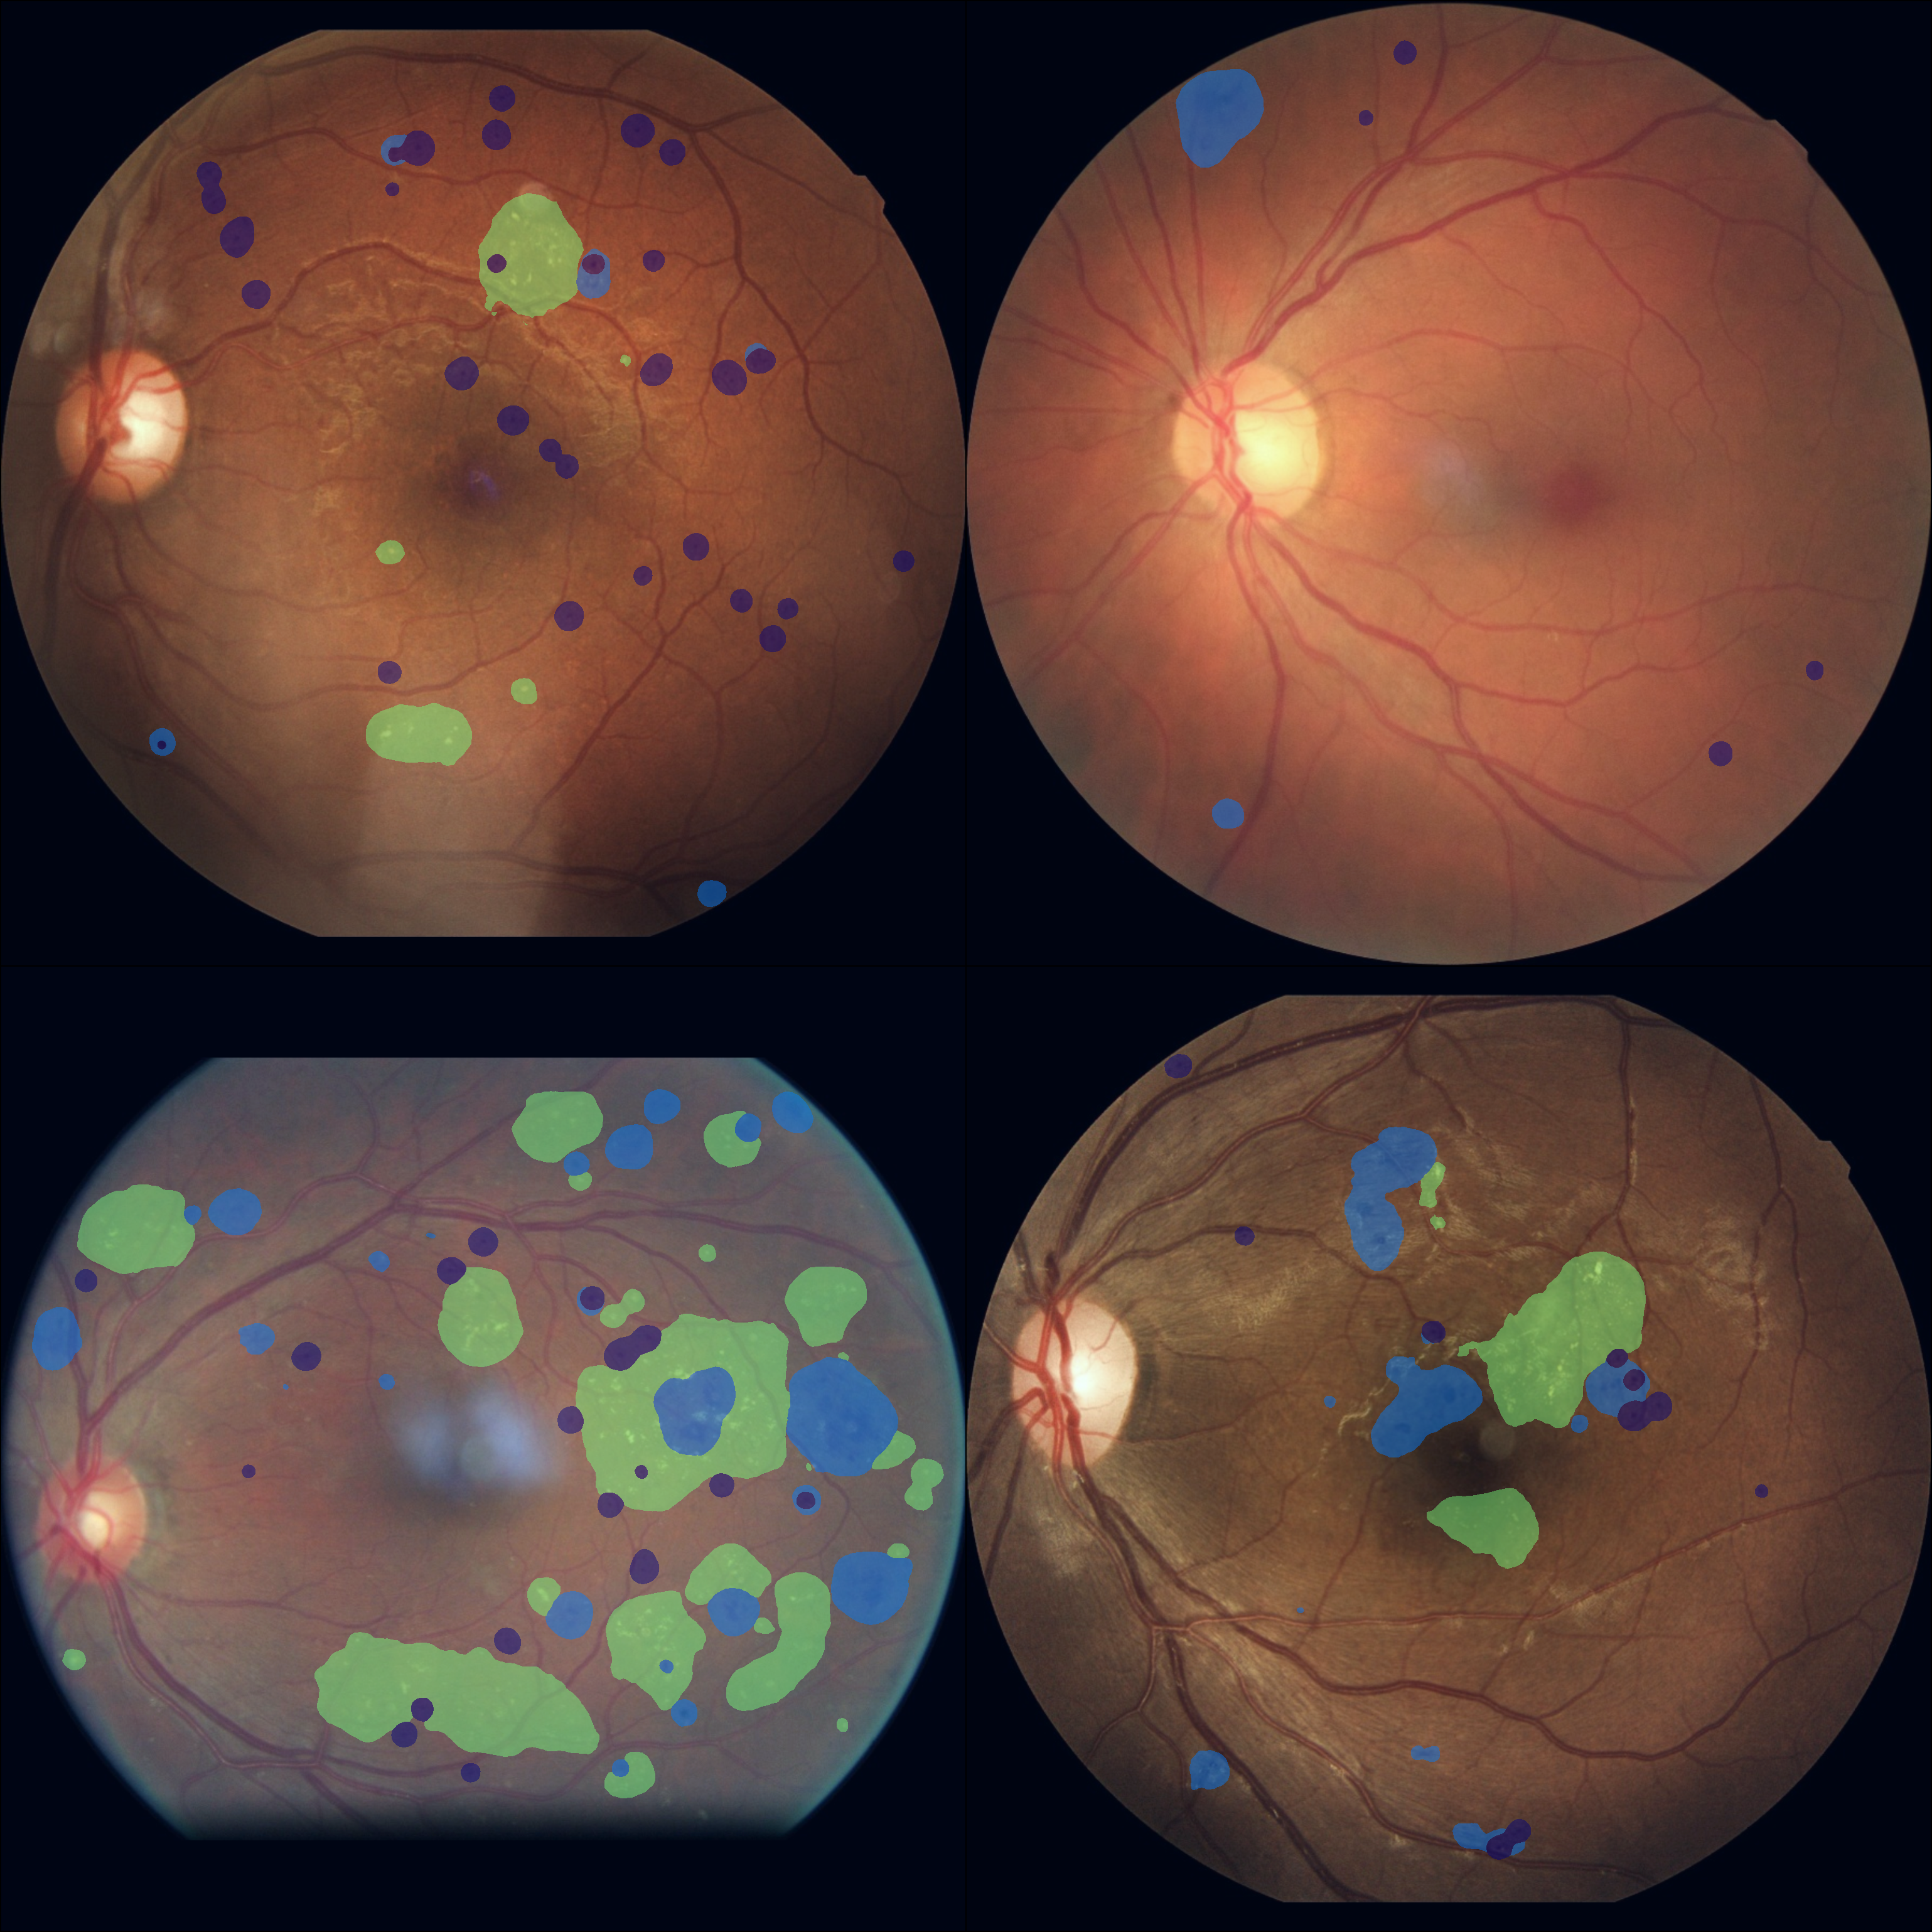
\includegraphics[width=\textwidth]{segmentation_lesions/generalisation/CombinedModelTricking/model_ALL_images_RETINAL_LESIONS_compression}
	\end{minipage} \\
		\bottomrule
	\end{tabular}
\end{table}


\subsubsection{Classification de l'origine de l'image}
L'approche par perturbations simples ne permettant pas d'expliquer le comportement du modèle, nous adoptons une méthode inspirée par les travaux de Alain et al. \cite{DBLP:conf/iclr/AlainB17}. Pour comprendre les caractéristiques lues par un modèle, ces derniers proposent d'inspecter les différentes couches d'un réseau en utilisant des sondes linéaires prenant pour entrée les cartes caractéristiques issues de chaque couche et tentant de les classifier. La linéarité de ces sondes n'est pas en soi indispensable mais elle confère un caractère interprétable. Par ailleurs, il est pertinent de garder un modèle simple de sonde car ce n'est pas son pouvoir discriminant qui présente un intérêt, mais celui des caractéristiques issues du réseau inspecté. \\
De façon équivalente, nous proposons d'entraîner un micro-modèle pour sonder les caractéristiques extraites de l'encodeur du modèle de segmentation. Ce dernier est gelé, autrement dit ses poids ne seront pas modifiés. Le positionnement de la sonde (c'est-à-dire la profondeur de la couche sondée dans l'encodeur) est un paramètre expérimental. La sonde a pour objectif de prédire l'origine de l'image d'entrée, c'est-à-dire sa base d'appartenance parmi les cinq que nous utilisons. Le modèle de sonde employé n'est pas linéaire pour des raisons pratiques de convergence mais il repose sur une architecture extrêmement simple. Nous l'illustrons sur la figure \ref{fig:ModeleSondeClassifDatabase}.
La sonde, dénotée $s$, est entraînée à minimiser la fonction d'entrophie croisée:
\begin{equation}
	\mathcal{L}(x_n, y_n) = \sum_{c=1}^{C} \log s(x_{n})_c \cdot y_{n, c}
\end{equation}
où $x_n$ est l'image d'entrée, $s(x_{n, c})$ la probabilité d'appartanence à la base de données $c$ prédite par le modèle et $y_{n, c}$ la vérité terrain.
\begin{figure}[h!]
	\centering
	\includegraphics[width=.8\textwidth]{segmentation_lesions/sonde_database}
	\caption{Modèle de sonde utilisé pour la classification de l'origine des données. Les flèches pointillées indiquent les différents points de connexion, mais il s'agit bien de quatre sondes distinctes, bien que basées sur la même architecture.}
	\label{fig:ModeleSondeClassifDatabase}
\end{figure}
 
En pratique, nous avons entraîné séparément différentes sondes, une par couche d'encodeur. Chacune d'entre elles est entraînée sur trois époques sur l'ensemble des données $\bigcup_i \mathcal{B}^{(i)}$. Les résultats sont fournis sur le graphique de la figure \ref{fig:classifDataset}. Pour en faciliter l'interprétation, nous avons équilibré les cinq classes (correspondant chacune à une base de données). Avec près de 97\% des images correctement classifiées dans le meilleur cas, force est de constater que la classification de l'origine des données ne pose pas problème à la sonde. La performance tend à s'améliorer fortement vers les couches les plus profondes du réseau de segmentation. Cela confirme la capacité du modèle à progressivement décoder ce marqueur dans l'image d'entrée. Dans le détail, notons que sur le graphique de la figure \ref{fig:classifDataset}, l'indice 0 correspond à l'image brute. Rien qu'à partir de celle-ci, la sonde prédit la base d'appartenance d'origine avec une exactitude de près de 60\%. Ce chiffre grimpe jusqu'à 97\% pour la sonde placée sur l'avant-dernière couche de l'encodeur. Pour celle-ci, nous étoffons notre analyse en calculant la matrice de confusion des prédictions réalisées, rapportée sur la figure \ref{fig:confMatProbeRef}. Dans le détail par classe, on observe que la plus grande source d'erreur provient d'images de MESSIDOR et IDRID (respectivement 28.4\% et 17.2\% de ces deux bases) prédites comme appartenant à DDR par la sonde. Cela témoigne a priori d'une grande proximité entre ces trois bases, en accord avec notre analyse préliminaire de la section \ref{sec:variabilitéSegmentation}.
Quoiqu'il en soit, l'existance d'un identifiant indiquant la base d'origine inscrit dans l'image et décodé progressivement par le modèle de segmentation se confirme à travers nos résultats.

\begin{figure}
	\centering
	\includegraphics[width=.7\textwidth]{segmentation_lesions/generalisation/accuracy_dataset_classif}
	\caption{Performance de classification de l'origine des images ($\mathcal{B}^{(i)}$) suivant la couche d'encodage sondée dans le modèle de segmentation.}
	\label{fig:classifDataset}
\end{figure}

\begin{figure}
	\centering
	\includegraphics[width=.7\textwidth]{segmentation_lesions/probing/probe_confMat}
	\caption{Matrice de confusion obtenue à partir des prédictions de la sonde située dans l'avant dernière couche d'encodage du modèle de segmentation.}
	\label{fig:confMatProbeRef}
\end{figure}


\paragraph{Adaptation par conversion adversariale}
La facilité de classification de l'origine de l'image par la sonde interroge sur les caractéristiques lues dans celle-ci permettant cette classification. Répondre à cette question offre indirectement une opportunité de premier choix: est-il possible de modifier l'image d'entrée de telle sorte à tromper la sonde? Si tel est le cas, l'effet se répercute-t-il sur le modèle de segmentation (décodeur inclus)? Enfin, ce faisant, peut-on le contraindre à adopter un style d'annotations choisi? \\

Pour étudier ces questions, nous avons mis au point une expérience basée sur le principe des attaques adversariales. Cette technique vise à modifier imperceptiblement l'entrée d'un réseau de telle sorte à le tromper dans sa classification et à détourner sa prédiction originale vers une classe cible choisie. Dans notre cas, l'attaque est portée sur la sonde de classification dans le but de lui faire prédire une base de données $T$ choisie sur n'importe quelle image qui lui est proposée. Les travaux existants sur les attaques adversariales suggèrent diverses modifications de l'image pour atteindre cet objectif. La plus courante est de rétro-propager les gradients de la fonction de coût évaluée sur la cible $T$ jusqu'à l'entrée. On modifie ensuite celle-ci par descente de gradients dans la direction qui minimise ce coût (et maximise donc la prédiction $T$). Il existe une abondante littérature sur le sujet, en général orientée vers la question de la cyber-sécurité des réseaux de neurones, car le principe des attaques adversariales repose sur l'exploitation d'une de leur vulnérabilité intrinsèque (la sensibilité au gradient). Notre application est transverse à ces questions, car notre objectif est de caractériser la capacité d'adaptation à divers domaines de distribution. Par ailleurs, nous souhaitons bien mettre l'accent sur le fait que l'attaque adversariale a ici pour but de tromper la sonde et non le modèle de segmentation. L'effet sur ce dernier, bien que nous verrons qu'il est radical, en est une conséquence indirecte.

Nous utilisons l'approche de Madry et al. \cite{DBLP:conf/iclr/MadryMSTV18} pour concevoir notre attaque:
soient $x$ l'image initiale (issue de $\mathcal{B}_{\star}$) et $t$ la classe que l'on souhaite faire prédire à la sonde. La création d'une image adversariale s'obtient suivant la procédure itérative suivante:
\begin{align}
	x_0 &= x \nonumber \\
	x_{k+1} &= \mathcal{S}_\epsilon(x_k - \alpha \cdot \text{signe}(\nabla \mathcal{L}(x_k, t))), k \in \left\lbrace 1,...,K
	\right\rbrace 
	\label{eq:adversarialExample}
\end{align}
où $\mathcal{S}_\epsilon$ est une fonction qui restreint la perturbation dans une boule centrée sur $x$ de rayon $\epsilon$. On reconnaîtra ici une équation très similaire à celle de la descente de gradients; précisons simplement qu'ici, seule l'image d'entrée est modifiée et non les poids ni de la sonde, ni du réseau de segmentation. L'équation \ref{eq:adversarialExample} se répète $K$ fois et l'image résultante $x_K$ est théoriquement censée perturber la prédiction de la sonde vers la classe choisie. Par ailleurs, en contraignant un $\epsilon$ petit, on force cette modification à rester imperceptible à l'\oeil{} humain. \\
Pour nos expériences, nous utilisons $\epsilon=0.025$, un pas de modification $\alpha = 0.002$ et $K=15$ étapes. Du fait du petit $\epsilon$, les perturbations sont a priori imperceptibles à l'\oeil{} humain: les valeurs de pixels de l'image étant comprises dans l'intervalle $\left[-1, 1\right]$, elles ne peuvent être modifiées au maximum que de $0.125\%$. \\
Pour simplifier la lecture des résultats, nous introduisons une nouvelle notation: $\mathcal{B}^{(i)} \Rightarrow \mathcal{B}^{(j)}$ indique une conversion adversariale des images de la base source $\mathcal{B}^{(i)}$ vers la base cible $\mathcal{B}^{(j)}$. Ainsi $M( \mathcal{B}_\star^{(j)} \Rightarrow \mathcal{B}^{(i)})$ signifie que le modèle $M$ est testé sur des images appartenant à $\mathcal{B}_\star^{(j)}$ qui ont été modifiées pour correspondre à la base  $\mathcal{B}^{(i)}$. Nous pouvons quantifier le succès de conversion, en observant la proportion d'images classées $T$ par la sonde après conversion $\bigcup_i \mathcal{B}^{(i)}_\star \Rightarrow \mathcal{B}^{(T)}$. Les résultats sont rapportés sur la figure \ref{fig:labelConversionSuccess}. Dépendamment de la cible $T$, le taux de conversion réussie varie entre  82.5\% (vers IDRID) et 65.2\% (vers MESSIDOR). Dans le détail, les images issues FGADR sont celles les plus difficilement converties, avec 15.3\% de conversion ratées provenant d'images de cette base (pour la conversion vers IDRID), 21.4\% (vers MESSIDOR) et 33.5\% (vers RETINAL-LESIONS). Si on exclue FGADR de nos images de test, le taux de succès de conversion moyen (toute base confondue) est de 90.5\%, le taux le plus faible étant pour la conversion vers FGADR (79\% de succès) et le plus élevé pour RETINAL-LESIONS (98.8\%).

\begin{figure}
	\centering
	\includegraphics[width=\textwidth]{segmentation_lesions/probing/accuracy_probe_after_convert}
	\caption{Pourcentage d'images des bases $\bigcup_i \mathcal{B}^{(i)}$ classées $T$ par la sonde après conversion $\bigcup_i \mathcal{B}^{(i)} \Rightarrow \mathcal{B}^{(T)}$. Cette proportion correspond au taux d'images ayant trompé la sonde après conversion vers la cible $T$ visée.}
	\label{fig:labelConversionSuccess}
\end{figure}

Cependant, tromper la sonde n'est pas notre objectif en soi. Dans le contexte de notre étude d'inter-généralisation, il est plus intéressant d'observer comment l'image transformée impacte la prédiction du modèle de segmentation. Dans le tableau \ref{tab:AdversarialAttackResult}, nous illustrons l'effet de la conversion sur le modèle. La sonde choisie est connectée à l'avant-dernière couche de l'encodeur et nous avons expérimenté avec deux types de conversions (vers IDRID et vers RETINAL-LESIONS). Considérant que toutes les segmentations du tableau sont réalisées avec le même modèle inchangé et sur des images de test, les résultats obtenus se révèlent déroutants: les modifications adversariales apportées à l'image d'entrée permettent de drastiquement modifier le style de segmentation. Ce faisant, nous obtenons une très grande flexibilité sur le style de segmentation en sortie: un même modèle peut-être configuré, sans avoir à le modifier et donc sans ré-entraînement coûteux, à adopter un style de segmentation parmi plusieurs alternatives. Qui plus est, le processus de conversion est stable: la conversion $\mathcal{B}^{(i)} \Rightarrow \mathcal{B}^{(i)}$ ne modifie pas la segmentation du modèle.

\renewcommand{\colSize}{0.40}
\begin{table}
	\caption{L'attaque adversariale de la sonde de classification modifie de manière imperceptible à l'\oeil{} nu l'image d'entrée. En revanche, elle permet de drastiquement modifier la segmentation pour adopter un style au gré de l'utilisateur.}
	\label{tab:AdversarialAttackResult}
	\begin{tabular}{m{2cm} cc}
		\toprule
		Modèles & \multicolumn{2}{|c}{Bases} \\
		\midrule
		& $\mathcal{B}^{(I)}_{\star}$ & $\mathcal{B}^{(R)}_{\star}$ \\
		
		$\mathcal{M}[\bigcup_i \mathcal{B}^{(i)}]$ (Référence) & 
		\begin{minipage}{\colSize\textwidth}
			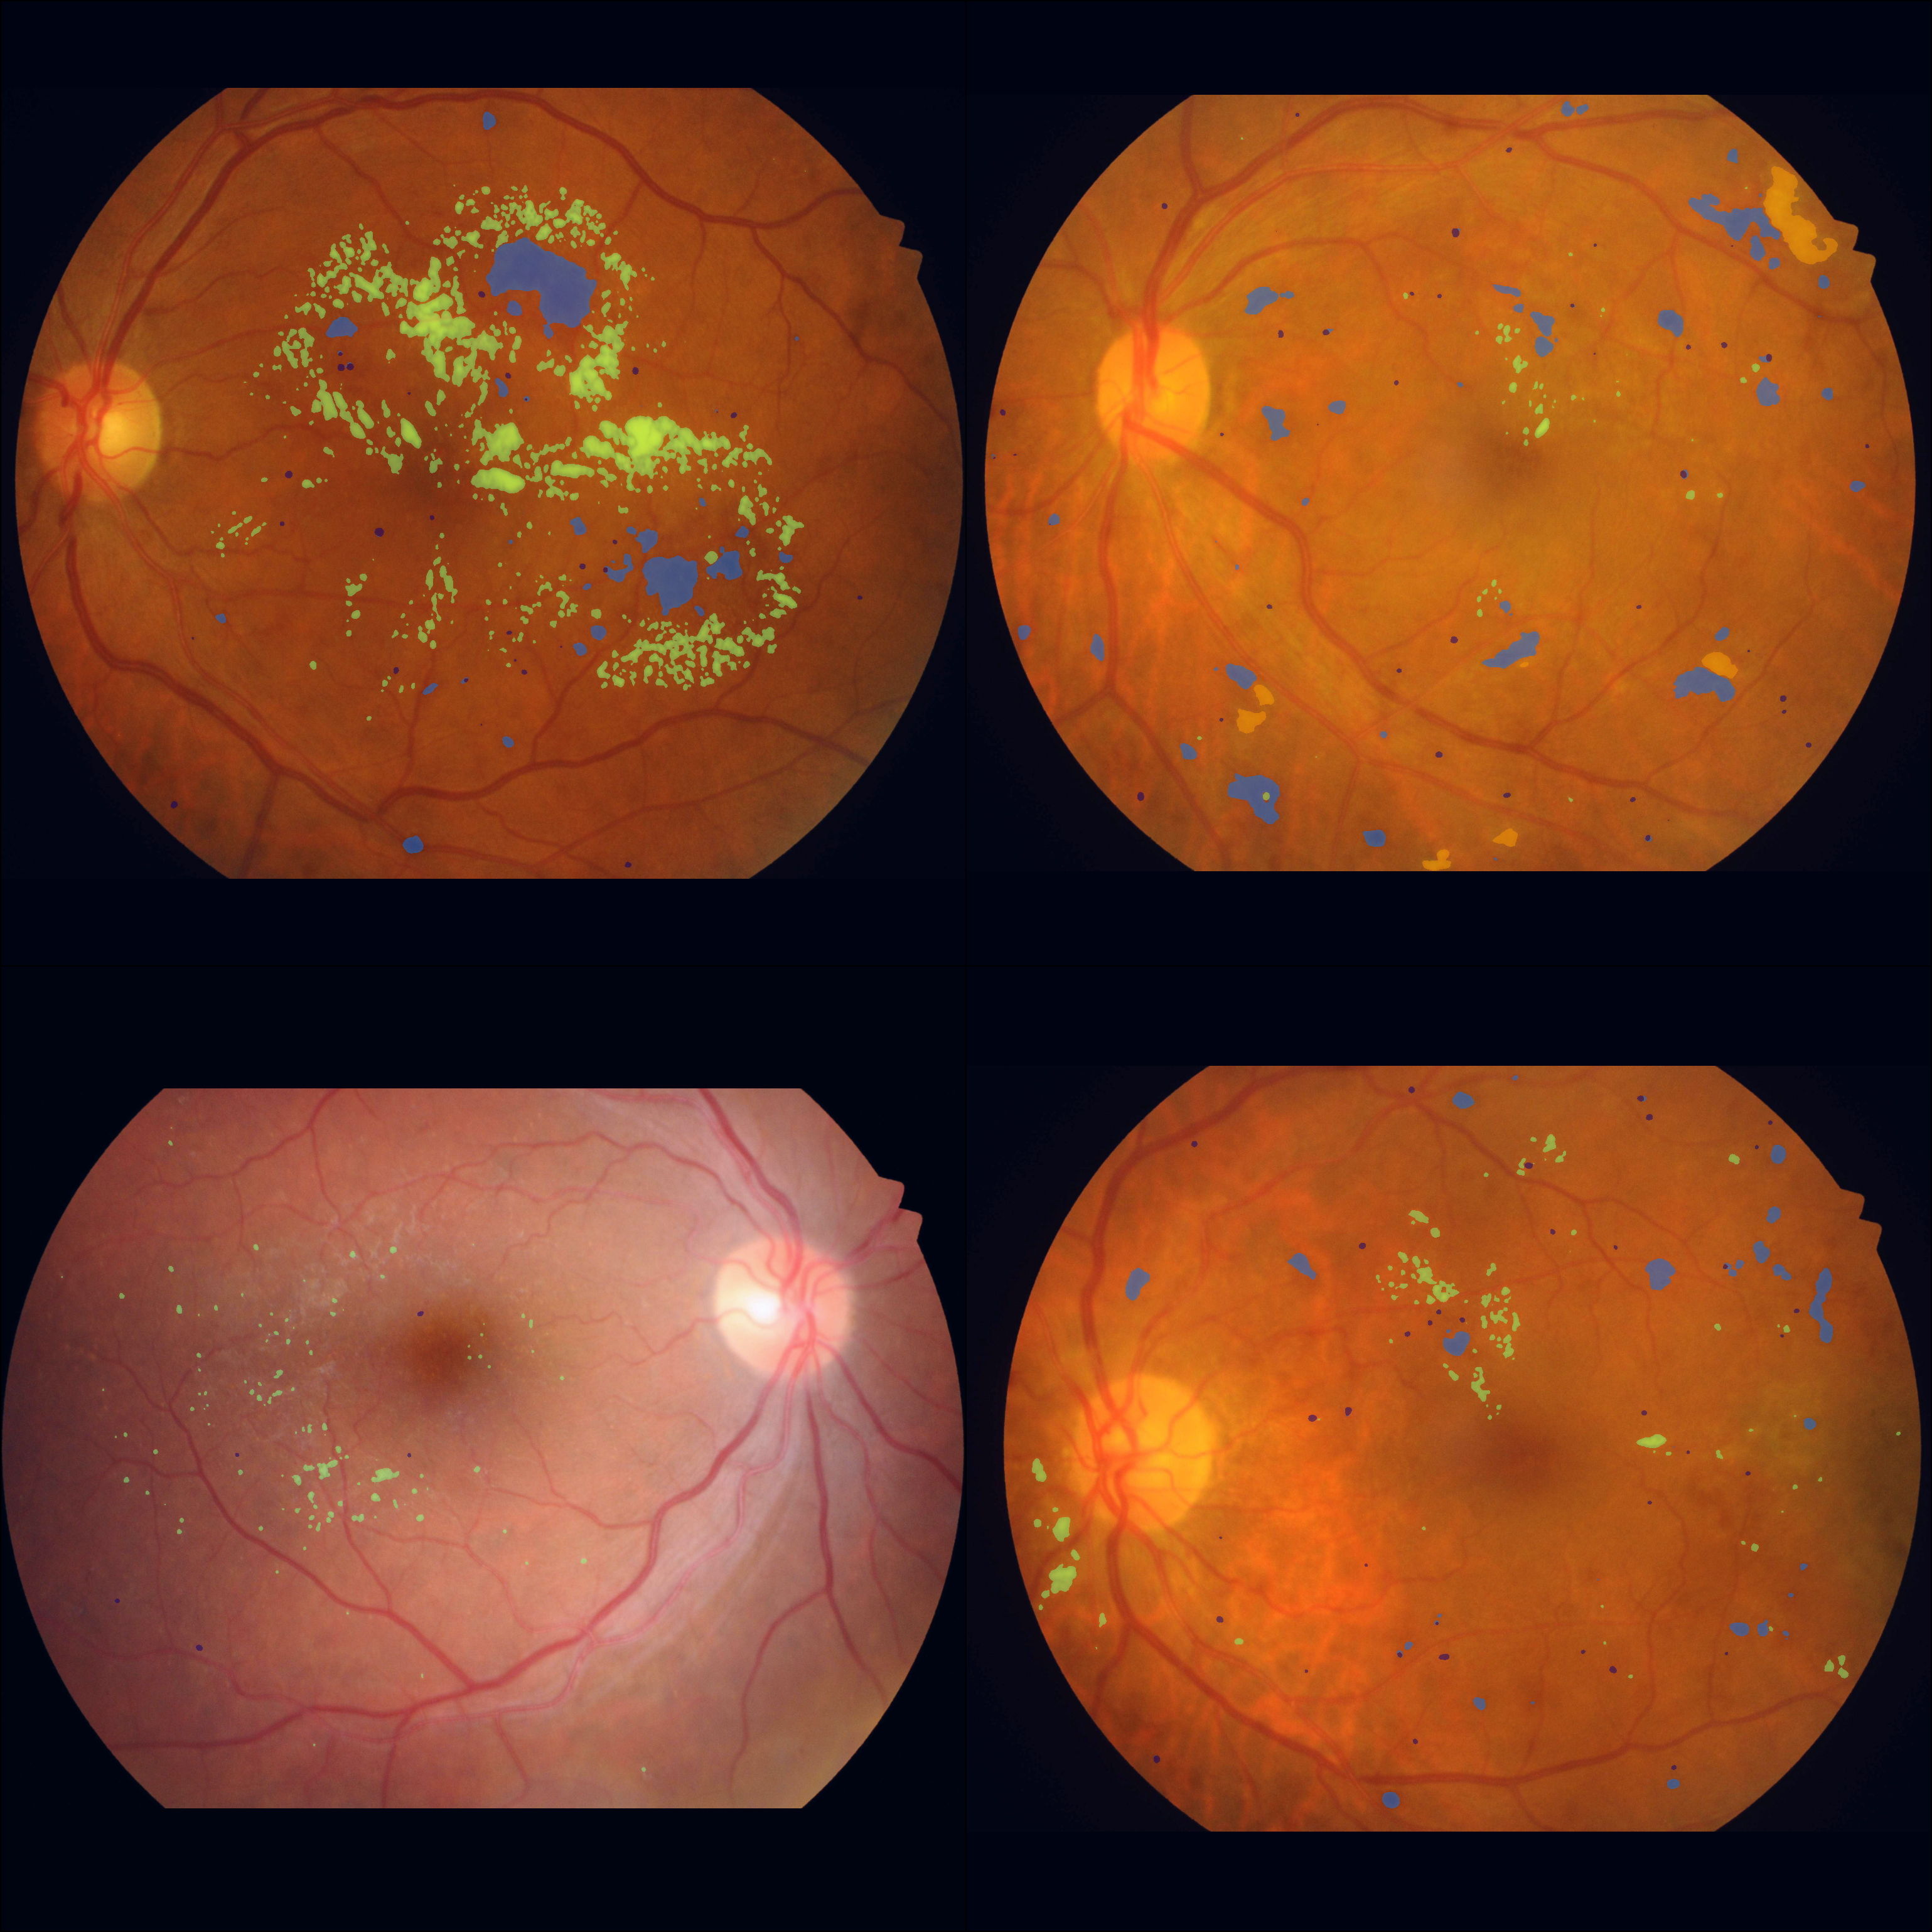
\includegraphics[width=\textwidth]{segmentation_lesions/generalisation/CombinedModelTricking/model_ALL_images_IDRID_ref}
		\end{minipage}
		& 
		\begin{minipage}{\colSize\textwidth}
			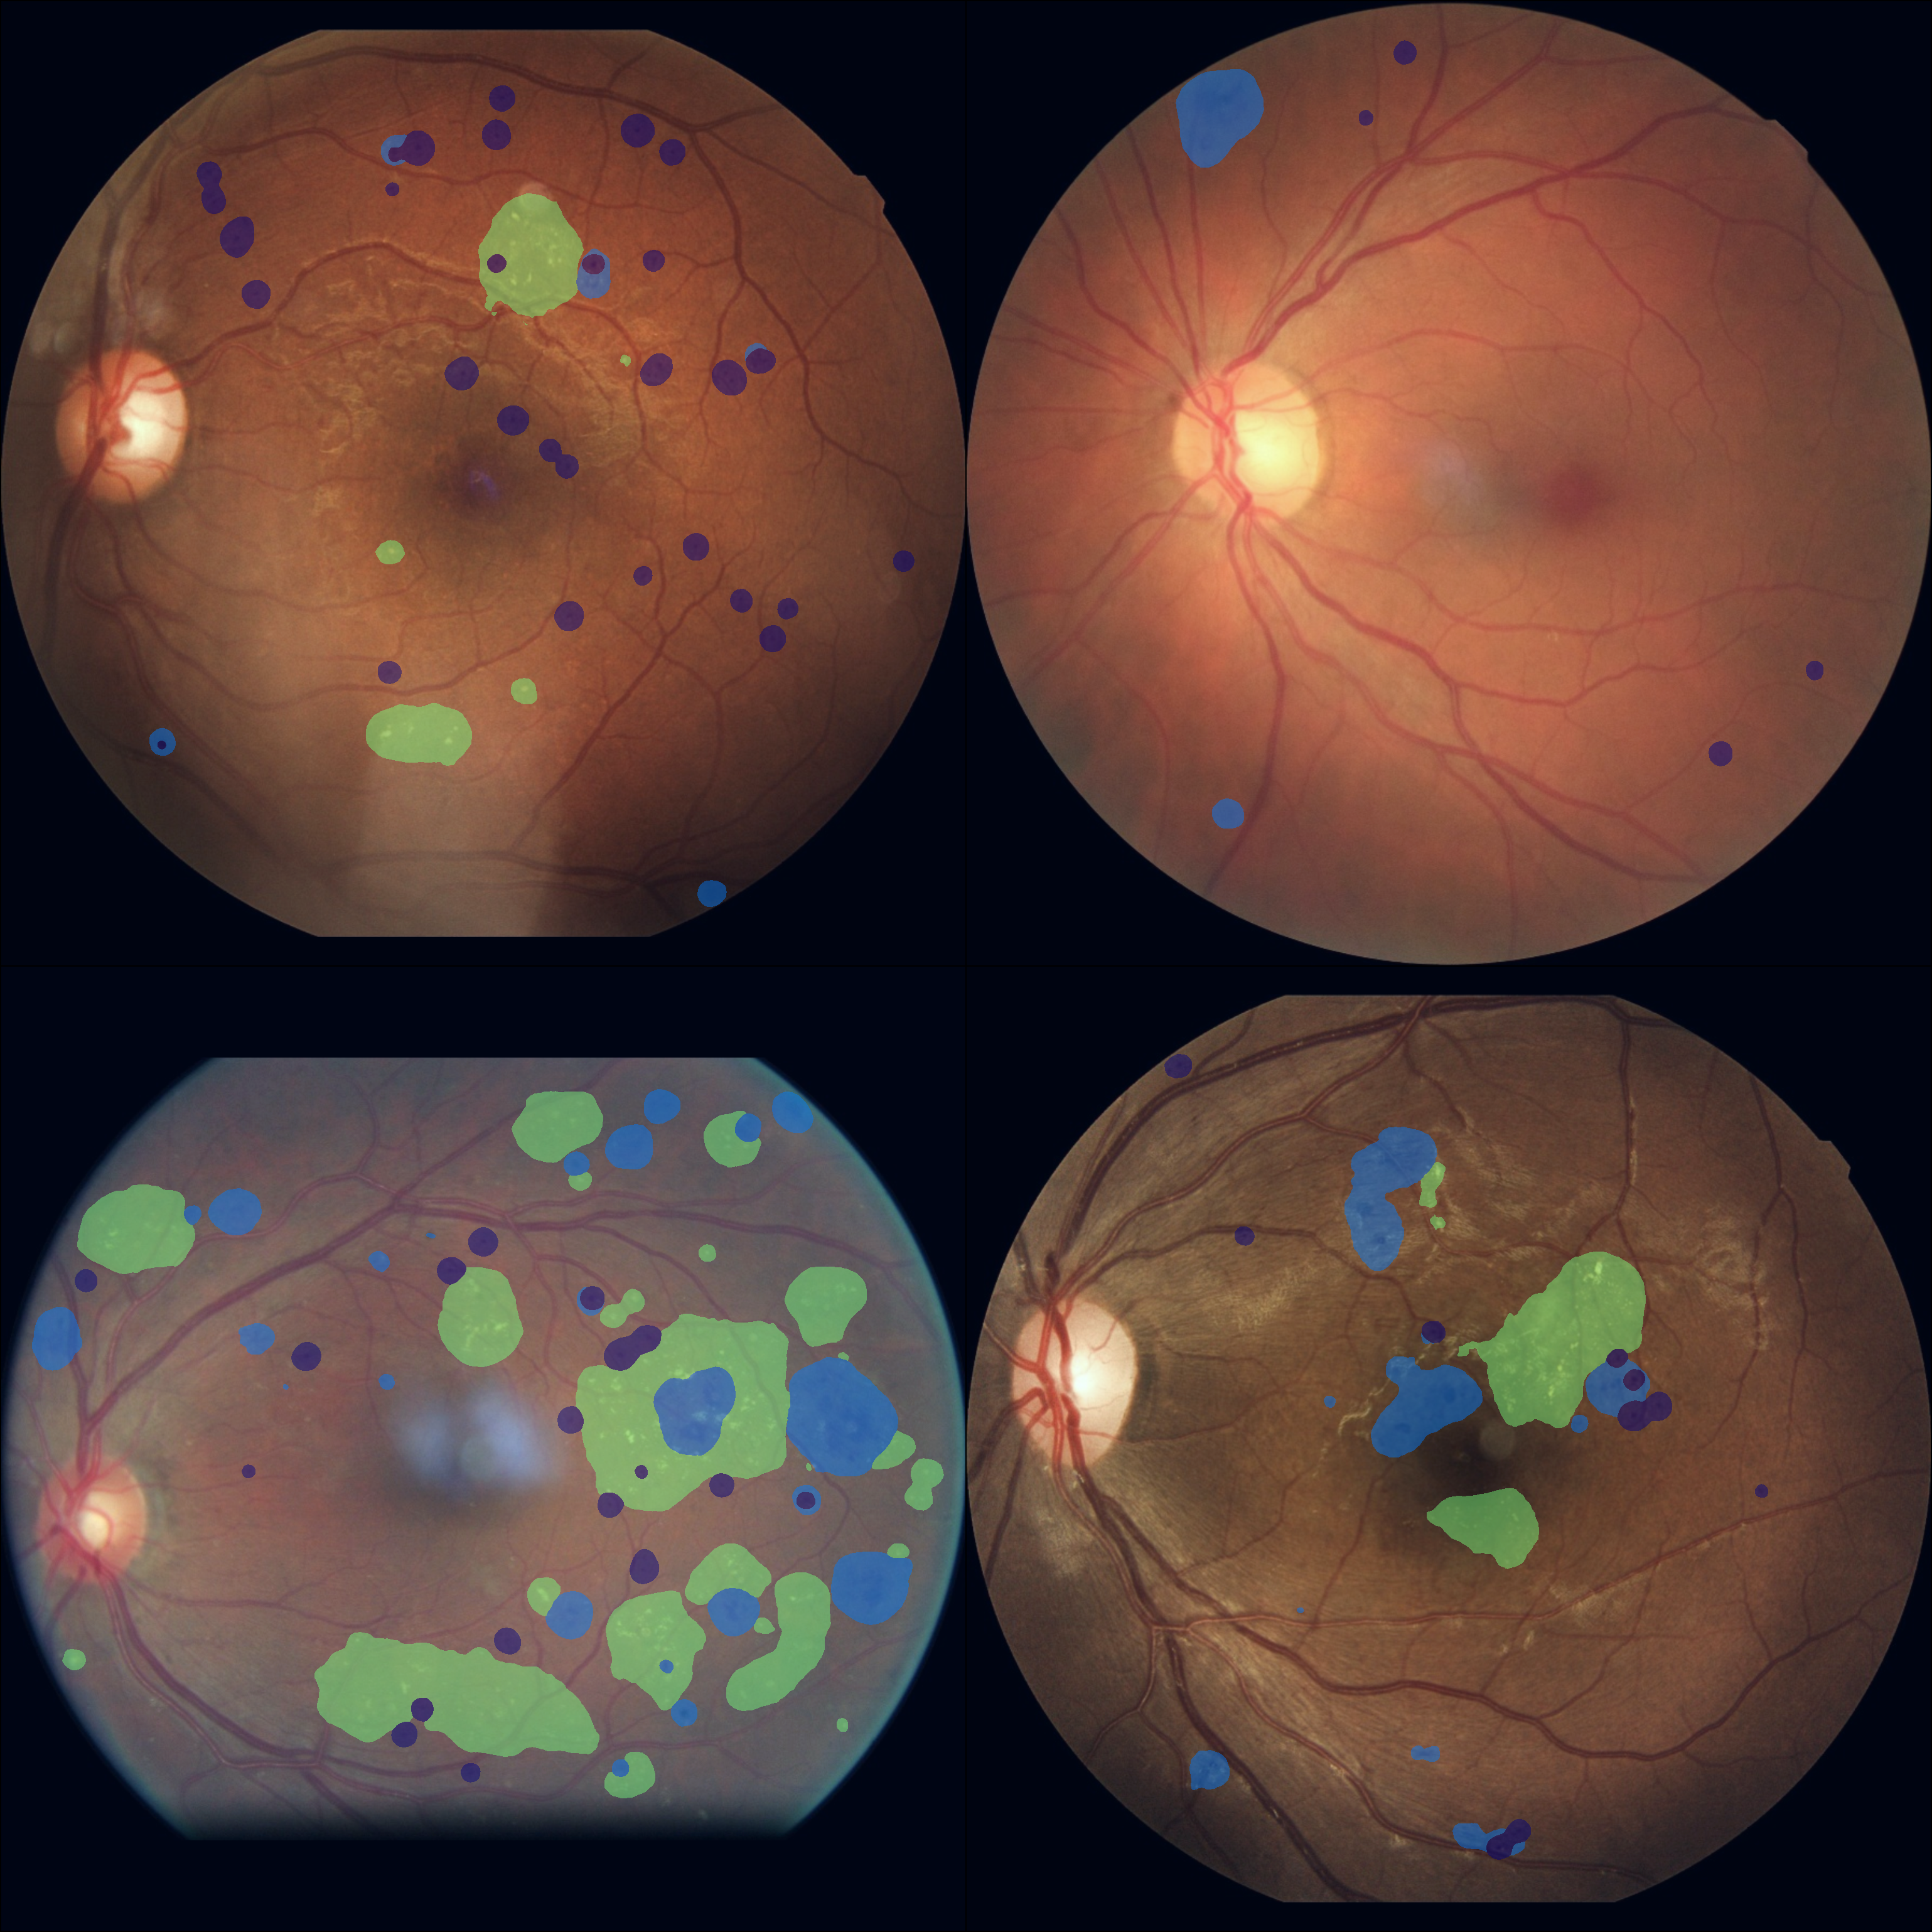
\includegraphics[width=\textwidth]{segmentation_lesions/generalisation/CombinedModelTricking/model_ALL_images_RETINAL_LESIONS_ref}
		\end{minipage}
		\\
		\midrule
		\midrule
		$\mathcal{M} \Rightarrow \mathcal{B}^{(I)} $ &
		\begin{minipage}{\colSize\textwidth}
			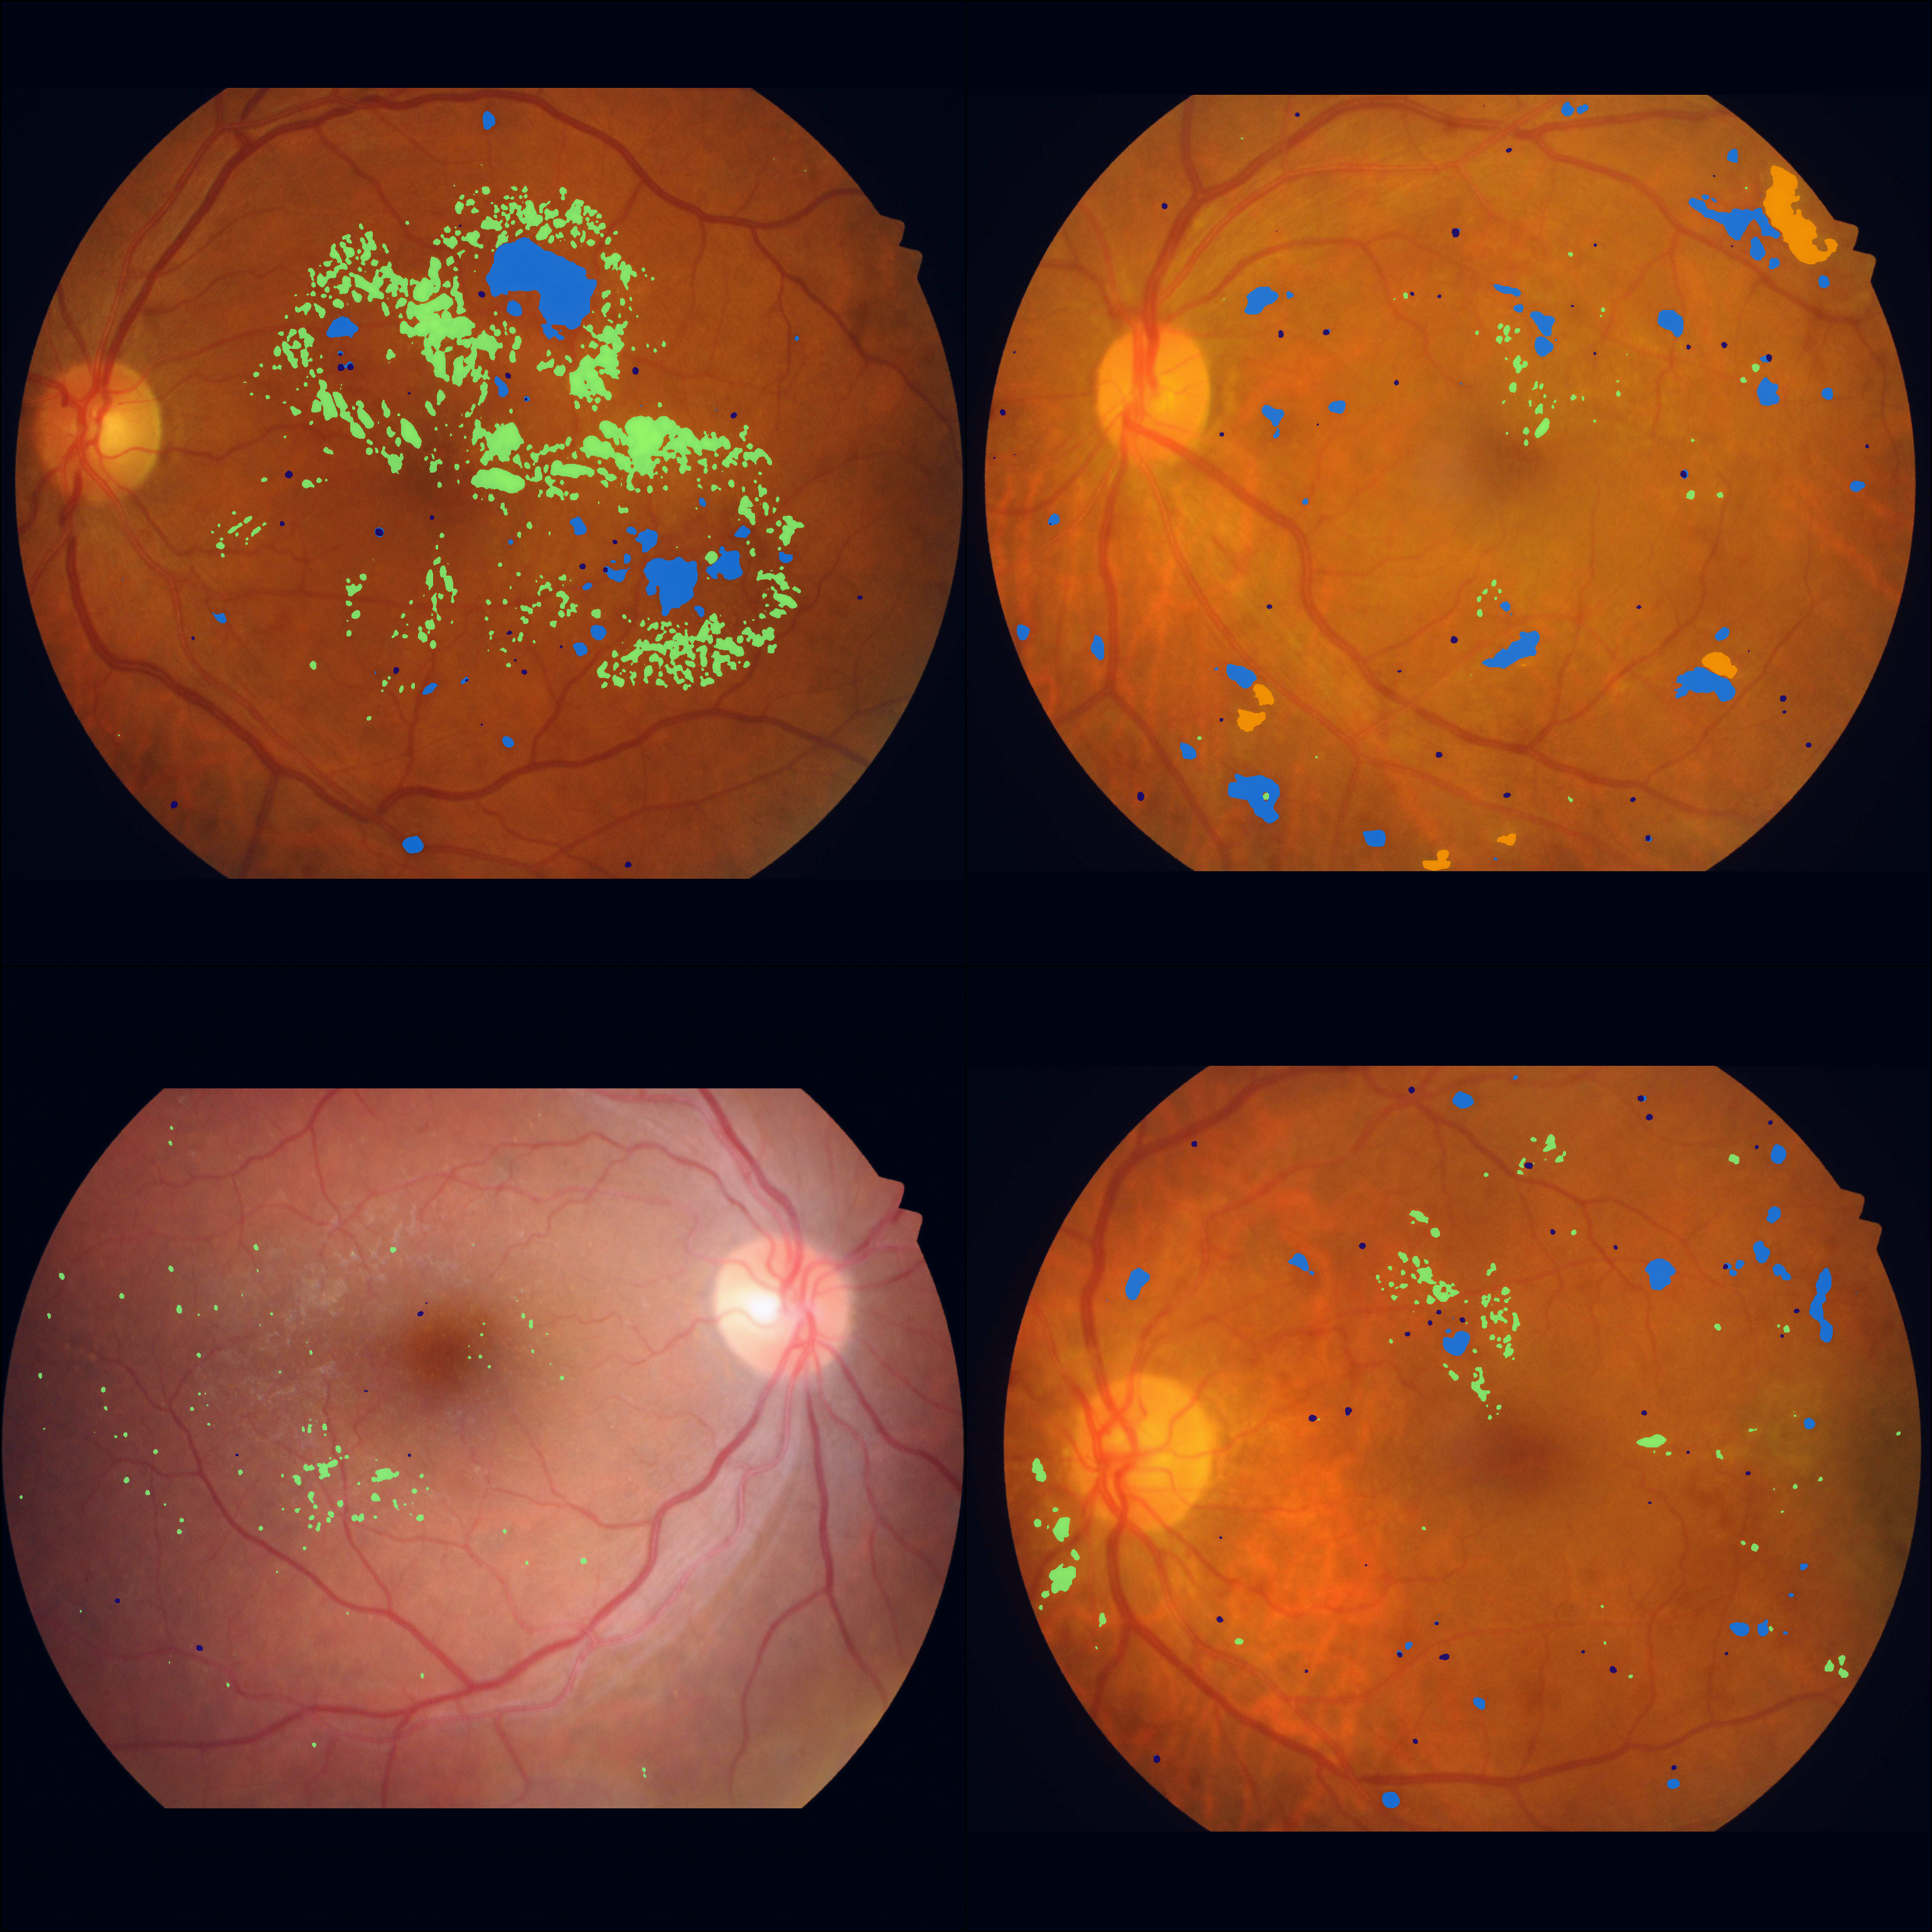
\includegraphics[width=\textwidth]{segmentation_lesions/generalisation/CombinedModelTricking/model_ALL_images_IDRID_adversarial_ref}
		\end{minipage}
		&
		\begin{minipage}{\colSize\textwidth}
			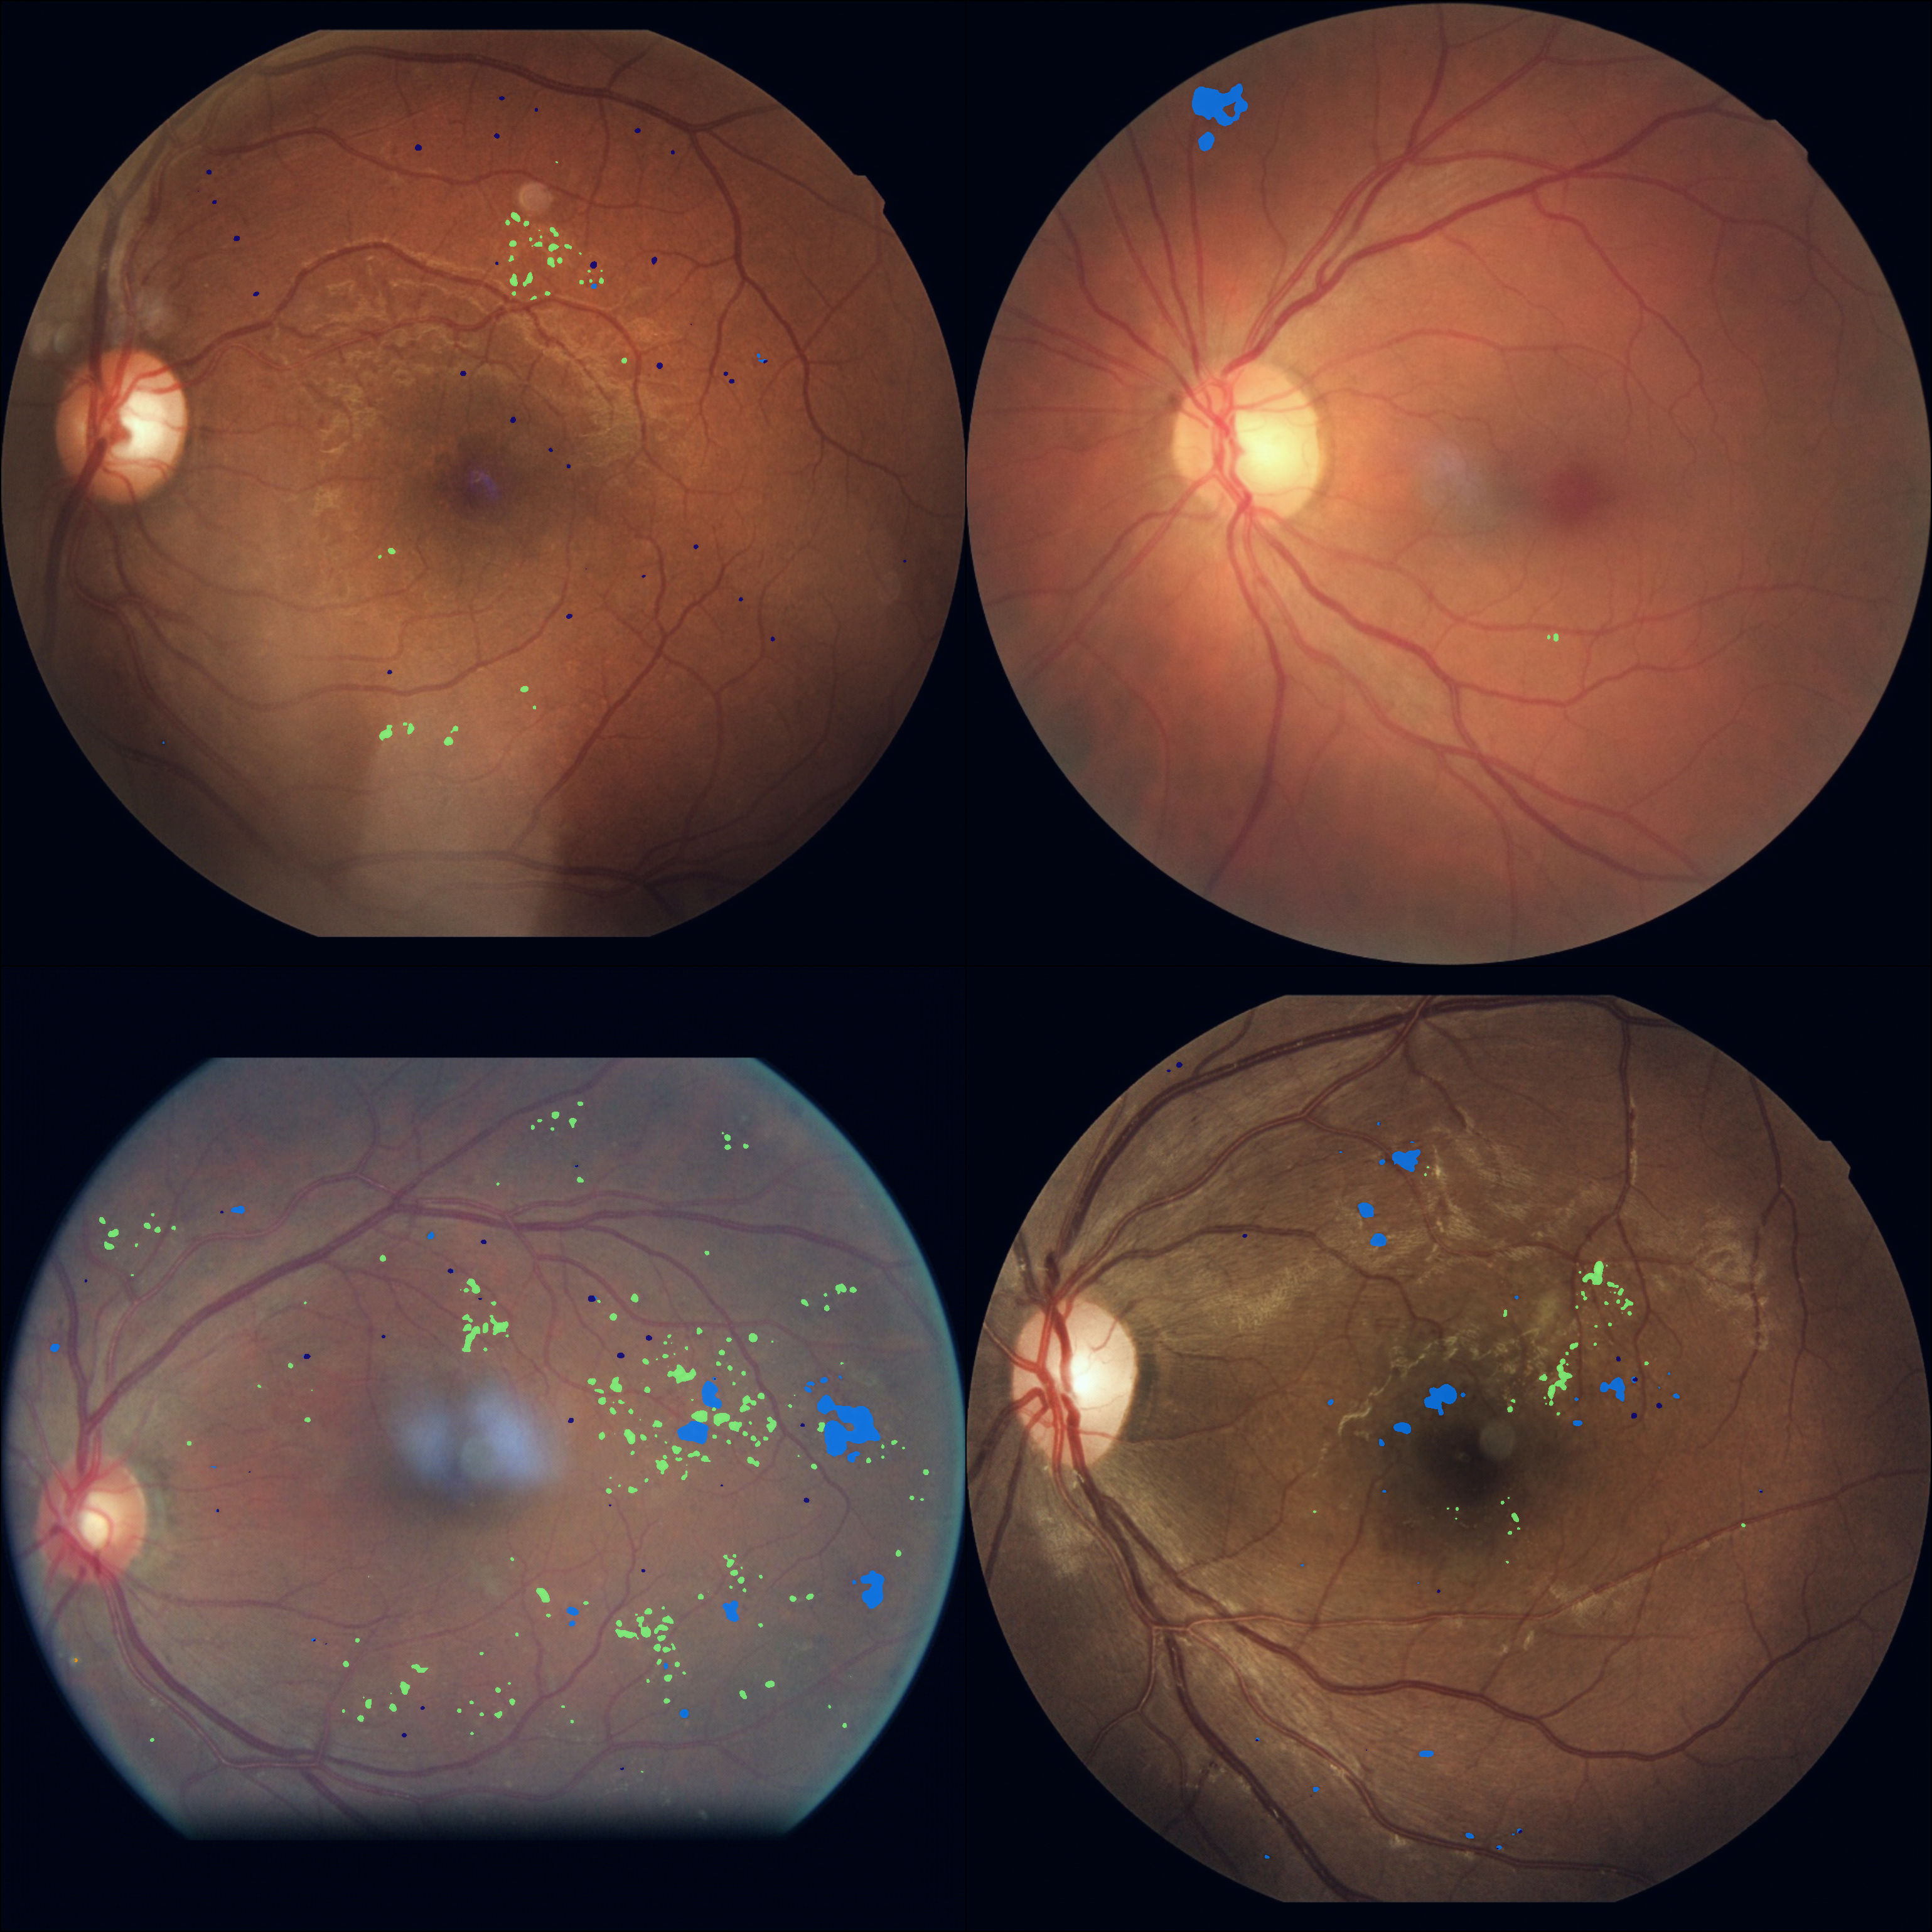
\includegraphics[width=\textwidth]{segmentation_lesions/generalisation/CombinedModelTricking/model_ALL_images_RETINAL_LESIONS_adversarial}
		\end{minipage} 
		\\
		\midrule
		$\mathcal{M} \Rightarrow \mathcal{B}^{(R)} $ &
		\begin{minipage}{\colSize\textwidth}
			\includegraphics[width=\textwidth]{segmentation_lesions/generalisation/CombinedModelTricking/model_ALL_images_IDRID_adversarial}
		\end{minipage}
		&
		\begin{minipage}{\colSize\textwidth}
			\includegraphics[width=\textwidth]{segmentation_lesions/generalisation/CombinedModelTricking/model_ALL_images_RETINAL_LESIONS_adversarial_ref}
		\end{minipage}
		\\
		\bottomrule
	\end{tabular}
\end{table}
 
\paragraph{Validation quantitative}

L'efficacité du processus de conversion des images reste encore à démontrer. À défaut d'avoir plusieurs styles d'annotations pour une même image, nous disposons de modèles dont nous savons qu'ils ont chacun adopté un style d'annotations spécifique (les $\mathcal{M}[\mathcal{B}^{(i)}]$). Ceux-ci nous serviront pour notre protocole d'évaluation. Notre objectif est d'éprouver la fiabilité du processus de conversion adversariale dans un contexte pseudo-clinique, donc sur des images qui n'appartiennent à aucune des bases utilisées jusqu'à présent. Nous prélevons pour cela un sous-ensemble de 100 images issues de la base APTOS, pour lesquelles nous ne disposons pas d'annotations de lésions. On note $\mathcal{K}$ cet ensemble. À partir de chacun des modèles $\mathcal{M}[\mathcal{B}^{(i)}]$, on génère cinq styles d'annotations de segmentations qui nous serviront de référence. Elles seront comparées avec les segmentations de $\mathcal{M}[\bigcup_i \mathcal{B}^{(i)}]$ après conversion adversariale vers chacune des bases. Formellement, notre validation repose donc sur l'évaluation de la métrique $D$ entre les modèles spécialisés et le modèle de référence après conversion des images vers le domaine de chaque modèle spécialisé:
\begin{equation}
	D(\mathcal{M}_{(j)}(\mathcal{K}), \mathcal{M}_\mathcal{S}(\mathcal{K} \Rightarrow \mathcal{B}^{(t)})), \forall j, t
\end{equation}
À l'instar de nos précédentes expériences, nous utilisons la mIoU comme métrique de comparaison. Les résultats sont synthétisés sur la matrice représentée sur la figure \ref{fig:ValidationConversionTable}. L'intérêt de ces résultats apparaît par une lecture ligne à ligne de la matrice fournie. En particulier, on observe que;
\begin{equation}
	D(\mathcal{M}_{(j)}(\mathcal{K}), \mathcal{M}_\mathcal{S}(\mathcal{K} \Rightarrow \mathcal{B}^{(j)})) \geq D(\mathcal{M}_{(j)}(\mathcal{K}), \mathcal{M}_\mathcal{S}(\mathcal{K} \Rightarrow \mathcal{B}^{(t)})), \forall j, t
\end{equation}
Autrement dit, après conversion vers la classe $T$, le modèle $\mathcal{M}_\mathcal{S} \Rightarrow T$ s'approche systématiquement le plus du modèle $\mathcal{M}_T$. Ce résultat confirme l'efficacité de l'approche adversariale pour modifier au choix le style de segmentation au modèle. 
\begin{figure}
	\centering
	\includegraphics[width=.6\textwidth]{segmentation_lesions/generalisation/validation_conversion}
	\caption{Cette matrice représente le score mIoU obtenu en comparant les prédictions réalisées par chacun des modèles spécialisés $\mathcal{M}_{(j)}$ et celles réalisées par le modèle $\mathcal{M}_\mathcal{S}$ après conversion adversariale des images d'entrées vers chacune des bases.}
	\label{fig:ValidationConversionTable}
\end{figure}


\subsection{Classification de la rétinopathie diabétique par \ac{GNN}}
Afin de pousser l'exploration sur la qualité des lésions, nous proposons de reconstituer le diagnostic de l'image à partir des cartes de segmentation produites par les différents modèles $\mathcal{M}[\mathcal{B}^{(i)}]$. Deux architectures de classification sont comparées, telles que décrites dans la section méthodologique. L'entraînement est réalisé sur les 35126 images de l'ensemble d'apprentissage de la base EyePACS. $5\%$ de ces images sont utilisées pour la validation du modèle. Le modèle qui obtient le meilleur score de validation au cours de 250 époques est ensuite évalué sur les bases Aptos et EyePacs (test). 
Les résultats sont  reportés dans le tableau \ref{tab:PerfGNNClassification}. En moyenne, quelque soit le modèle de segmentation (hormis celui entraîné sur IDRiD), l'architecture Att-GNN obtient les meilleures performances. Notamment, ce constat est particulièrement notable sur l'ensemble de test EyePacs, composé d'images de bien moins bonne qualité que sur Aptos.
\\
Dans le détail, on observe également la supériorité (en moyenne sur les deux ensembles) des performances obtenues avec $\mathcal{M}_\mathcal{S}$ obtenant respectivement 0.735 (Att-GNN) et 0.682 (PointNet++), suivi de $\mathcal{M}[\mathcal{B}^{(R)}]$ (scores respectivement de 0.714 et 0.663). \\
Relativement à ce que produit un CNN à partir d'une image, ces scores ne sont pas élevés, notamment par rapport à ceux obtenus dans l'étude préliminaire de la section \ref{sec:preliminaryExperimentClassSegm}. En les analysant plus finement, il apparaît que les modèles par graphe peinent surtout à distinguer certaines classes, en particulier la rétinopathie proliférative. Ce phénomène n'est pas surprenant, dans la mesure où ce grade de la maladie se détecte par l'apparition de néo-vaisseaux; or, nos modèles de segmentation ne sont pas entraînés à détecter ceux-ci. Pour mieux quantifier le potentiel de l'approche par graphe, nous simplifions donc le problème posé, en regroupant les classes 0 et 1 d'une part (non malade et bénigne) et les classes 2,3,4 d'autre part (modérée, sévère et proliférative.) Ce choix correspond aux recommandations dans le cadre de campagne de dépistage de la \ac{RD}. On obtient alors les performances reportées dans le tableau \ref{tab:DetectionRDScoreGraph}. Dans le meilleur des cas, nous obtenons un couple Sensibilité/Spécificité de détection de 96.57\%/81.29\% sur Aptos et de 52.77\%/98.06\% sur EyePacs. On peut s'étonner d'une telle différence de sensibilité entre les deux bases: elle s'explique notamment par le fait que la base EyePACS contient notoirement énormément d'images de mauvaises qualités. Sur celles-ci, le réseau de segmentation tend à sous-segmenter les lésions en raison de la faible lisibilité de l'image. Inversement, Aptos est plus homogène, on obtient donc de meilleurs résultats de segmentation dessus. Ce dernier point confirme donc la nécessité d'utiliser des images de bonne qualité dès lors qu'on utilise la segmentation pour classifier les images de \fundus{}.

\begin{table}
	\caption{Performances de classification (gradation en 5 classes) de la rétinopathie diabétique) à partir du graphe de lésions issu des différents modèles de segmentation. Deux architectures de classification sont comparées. On mesure le coefficient $\kappa$ de Cohen quadratique sur deux ensembles d'évaluation distincts.}
	\label{tab:PerfGNNClassification}
	\begin{subtable}{.48\textwidth}
		\caption{Score obtenu par le PointNet++}
	\begin{tabularx}{\textwidth}{X|lll}
		\toprule
		 Graphe issu de: & $\kappa$ Aptos &  $\kappa$ EyePACS & Moy.\\
		\midrule
		$\mathcal{M}[\mathcal{B}^{(I)}]$ & 0.345 & 0.240 & 0.293\\
		 $\mathcal{M}[\mathcal{B}^{(M)}]$ & 0.409 & 0.412 & 0.411\\
		 $\mathcal{M}[\mathcal{B}^{(D)}]$ & 0.782 & 0.474 & 0.628\\
		 $\mathcal{M}[\mathcal{B}^{(R)}]$ & 0.791 & 0.535 & 0.663\\
		 $\mathcal{M}[\mathcal{B}^{(F)}]$ & 0.554 & 0.281 & 0.418\\
		 $\mathcal{M}_\mathcal{S}$ & \textcolor{red}{\textbf{0.815}} & \textcolor{red}{\textbf{0.549}} & \textcolor{red}{\textbf{0.682}}\\
		\bottomrule
	\end{tabularx}
\end{subtable}
\hfill
\begin{subtable}{.48\textwidth}
	\caption{Score obtenu par le Attn-GNN}
	\begin{tabularx}{\textwidth}{X|lll}
		\toprule
		Graphe issu de: & $\kappa$ Aptos &  $\kappa$ EyePACS & Moy. \\
		\midrule
		$\mathcal{M}[\mathcal{B}^{(I)}]$ & 0.206 & 0.206 & 0.206\\
		$\mathcal{M}[\mathcal{B}^{(M)}]$ & 0.755 & 0.551 & 0.653 \\
		$\mathcal{M}[\mathcal{B}^{(D)}]$ & 0.801 & 0.505 & 0.653\\
		$\mathcal{M}[\mathcal{B}^{(R)}]$ & \textcolor{blue}{\textbf{0.822}} & 0.606 & 0.714\\
		$\mathcal{M}[\mathcal{B}^{(F)}]$ & 0.602 & 0.314 & 0.458\\
		$\mathcal{M}_\mathcal{S}$ & 0.789 & \textcolor{blue}{\textbf{0.682}} & \textcolor{blue}{\textbf{0.736}}\\
		\bottomrule
	\end{tabularx}
\end{subtable}
\end{table}

\begin{table}
	\caption{Performances de classification binaire dans un contexte de détection de la rétinopathie diabétique.}
	\label{tab:DetectionRDScoreGraph}
	\centering
	\begin{tabular}{ll|ll|ll|ll}
		\toprule
		GNN & Graphe issu de: & \multicolumn{2}{c}{Exactitude} & \multicolumn{2}{c}{Sensibilité} & \multicolumn{2}{c}{Spécificité} \\
		\midrule
		&& Aptos & EyePacs& Aptos & EyePacs& Aptos & EyePacs \\
		\midrule
		\multirow{2}{2cm}{PointNet} & $\mathcal{M}[\mathcal{B}^{(R)}]$ & 0.898 & 0.869 & 0.872 & 0.368 & \textbf{0.916} & \textbf{0.988} \\ 
		& $\mathcal{M}_\mathcal{S}$& 0.899 & 0.871 & 0.954 & 0.401 & 0.861 & 0.983 \\
		\midrule 
		\multirow{2}{2cm}{Att-GNN} &$\mathcal{M}[\mathcal{B}^{(R)}]$& \textbf{0.906} & 0.875 & 0.925 & 0.422 & 0.893 & 0.983 \\ 
		&$\mathcal{M}_\mathcal{S}$& 0.875 & \textbf{0.894} & \textbf{0.966} & \textbf{0.528} & 0.813 & 0.981 \\
		\midrule
	\end{tabular}
\end{table}

\subsubsection{Analyse des performances suboptimales de $\mathcal{M}[\mathcal{B}^{(I)}]$} 
Dans le tableau \ref{tab:PerfGNNClassification}, les graphes issus des modèles entraînés sur \ac{IDRiD} et dans une moindre mesure sur MESSIDOR se démarquent particulièrement des autres pour leurs mauvaises performances de classification. Or, jusqu'ici, rien ne permettait d'affirmer que ce modèle produisait de plus mauvaises segmentations que les autres. Considérant que la difficulté à juger de la pertinence clinique des métriques de segmentation était la principale motivation derrière notre travail de classification; nous pouvons déjà conclure à cet égard sur leur inadéquation relative à la classification par graphes. \\
Cependant, il existe une façon très simple d'améliorer ces résultats: connaissant la tendance de $\mathcal{M}[\mathcal{B}^{(I)}]$ à sur-segmenter les petites structures (du fait du style d'annotations de sa base d'entraînement), nous avons ré-entraîné le modèle Att-GNN sur le graphe de lésions issu de ce modèle mais en filtrant cette fois les lésions de taille inférieure à un certain seuil $t$. Les résultats sont affichés sur la figure \ref{fig:SizeFilteringLesionGNN}. Il y apparaît clairement que c'est la surabondance de \noeud{}s dans le graphe qui cause la dégradation des performances. Dès lors, rien qu'en filtrant toutes les structures de moins de 64 pixels, le score de classification sur Aptos est triplé. Malgré cette technique, le modèle n'atteint jamais les performances obtenues avec $\mathcal{M}_\mathcal{S}$; ce levier d'action reste donc limité.
\begin{figure}
	\centering
	\includegraphics[width=\textwidth]{segmentation_lesions/GNN/filter_size_effect_idrid}
	\caption{Effet du filtrage des plus petites structures segmentées par $\mathcal{M}[\mathcal{B}^{(I)}]$ sur la classification par graphe.}
	\label{fig:SizeFilteringLesionGNN}
\end{figure}
\subsubsection{Classification des images après conversion adversariale}
Un autre point qui mérite notre attention concerne l'efficience de classification avec le modèle $\mathcal{M}[\mathcal{B}^{(R)}]$. Ses performances ne surpassent pas celles de $\mathcal{M}[\mathcal{S}]$, mais elles s'en approchent malgré tout (voir les dépassent sur Aptos). Or, lors de l'analyse des résultats de segmentation, $\mathcal{M}[\mathcal{S}]$ se révélait bien supérieur à $\mathcal{M}[\mathcal{B}^{(R)}]$ (tableau \ref{tab:generalisationPerfSegmentation}). Cela suggère que malgré sa segmentation de moins bonne qualité, le style d'annotation du modèle entraîné sur la base $\mathcal{B}^{(R)}$ est propice à la classification. Or, rappelons qu'il s'agit du style produisant les segmentations les plus grossières (regroupant en de larges régions les structures voisines): comme notre graphe est construit sur la base d'un \noeud{} par structure connectée, une telle segmentation mène à une représentation par graphe bien plus allégée. Après avoir converti les images suivant notre schéma d'attaque adversariale, nous avons re-extraits les graphes et ré-entraînés les modèles. Les résultats sont synthétisés dans le tableau \ref{tab:GraphClassificationAfterConversion}. Ils ne dévoilent pas de tendances très claires: les performances sur Aptos sont légèrement améliorées après la conversion vers RETLES mais nettement détériorées sur EyePACS. En revanche, la modèle entraîné sur le graphe issu de $\mathcal{M}_\mathcal{S} \Rightarrow I$ se révèle bien plus efficace que $\mathcal{M}_I$ (mais bien moins que $\mathcal{M}_\mathcal{S}$):
\begin{align*}
	& \kappa^{Aptos}_{\mathcal{M}_R} > \kappa^{Aptos}_{\mathcal{M}_\mathcal{S} \Rightarrow R} > \kappa^{Aptos}_{\mathcal{M}_\mathcal{S}} > \kappa^{Aptos}_{\mathcal{M}_\mathcal{S} \Rightarrow I} > \kappa^{Aptos}_{\mathcal{M}_I}\\
	&\kappa^{EyePACS}_{\mathcal{M}_I} < \kappa^{EyePACS}_{\mathcal{M}_\mathcal{S} \Rightarrow I} < \kappa^{EyePACS}_{\mathcal{M}_R} < \kappa^{EyePACS}_{\mathcal{M}_\mathcal{S} \Rightarrow R} < \kappa^{EyePACS}_{\mathcal{M}_\mathcal{S}}
\end{align*}
La conversion adversariale se comporte donc comme une forme de modèle intermédiaire entre le modèle généraliste et le spécialisé, observation qui est d'ailleurs en adéquation avec les résultats de segmentation. 
\begin{table}
	\caption{Performances obtenues après conversion adversariale vers le style d'annotations de RET-LES et IDRID. Pour cette dernière, nous donnons également les scores avec un graphe élagué des lésions de moins de 64 pixels.}
	\label{tab:GraphClassificationAfterConversion}
	\begin{subtable}{0.51\textwidth}
		\caption{Gradation (classification multiclasses de R0 à R4)}
		\begin{tabularx}{\textwidth}{X|lll}
			\toprule
			Graphe issu de: & $\kappa^{Aptos}$  &  $\kappa^{EyePACS}$  & Moyenne \\
			\midrule
			$\mathcal{M}_\mathcal{S}$ & 0.789 & \textbf{0.682} & \textbf{0.736} \\
			$\mathcal{M}_\mathcal{S} \Rightarrow R$ & \textbf{0.795} & 0.613 & 0.704 \\
			$\mathcal{M}_\mathcal{S} \Rightarrow I$ & 0.657  & 0.458 &  0.558 \\
			$\mathcal{M}_\mathcal{S}\Rightarrow I^{(64)}$ & 0.731  & 0.476 &  0.604 \\
			\bottomrule
		\end{tabularx}
	\end{subtable}
\hfill
	\begin{subtable}{0.48\textwidth}
		\caption{Détection (classification R0-R1 vs R2-R3-R4)}
		\begin{tabularx}{\textwidth}{ll|ll|ll}
			\toprule
			\multicolumn{2}{c}{Ex.} & \multicolumn{2}{c}{Sens.} & \multicolumn{2}{c}{Spéc.} \\
			Apt. & Eye. & Apt. & Eye.& Apt. & Eye. \\
			\midrule
			0.875 & \textbf{0.894} & \textbf{0.966} & \textbf{0.528} & 0.813 & \textbf{0.981} \\
			\textbf{0.888} & 0.877 & 0.956 & 0.483 & \textbf{0.841} & 0.970 \\
			0.854 & 0.850 & 0.950 & 0.314 & 0.788 & 0.978 \\
			0.866 & 0.856 & 0.961 & 0.337 & 0.801 & 0.979 \\
			\bottomrule
		\end{tabularx}
	\end{subtable}
\end{table}
On a représenté sur la figure \ref{fig:aptos1} trois exemples de graphes construits depuis les prédictions de $\mathcal{M}_\mathcal{S}, \mathcal{M}_\mathcal{S} \Rightarrow R $ et $\mathcal{M}_\mathcal{S} \Rightarrow I$. Rappelons qu'il s'agit bien du même modèle, inchangé, prenant pour entrée la même image mais avec différentes conversions adversariales (non perceptibles visuellement).
\begin{figure}
	\centering
	\includegraphics[width=\linewidth]{segmentation_lesions/GNN/graphs/aptos_1}
	\includegraphics[width=\linewidth]{segmentation_lesions/GNN/graphs/aptos_2}
	\includegraphics[width=\linewidth]{segmentation_lesions/GNN/graphs/aptos_3}
	\caption{Exemples de graphes extraits à partir d'un même modèle $\mathcal{M}_\mathcal{S}$ avec ou sans conversion adversariale des images vers IDRID ou RETLES. Sur ces images, chaque \noeud{} est connectée à ses $k=3$ plus proches voisins mais elle est simplement indicative. Dans nos expériences de classification, $k=24$.}
	\label{fig:aptos1}
\end{figure}
\section{Discussion}
\subsection{Rappel des résultats obtenus}
Nous rappelons les principaux résultats de ce chapitre en dix points-clés:
\begin{enumerate}
	\item Nous proposons une caractérisation et une comparaison de bases de données publiquement disponibles, à la fois dans leur structure et dans leur style d'annotations.
	\item L'architecture de segmentation sémantique développée obtient des performances de paire avec l'état de l'art. Nous n'observons pas de différences très marquées entre un modèle spécifiquement conçu pour le \fundus{} et des modèles de segmentation plus généralistes.
	\item Même en maximisant un score sur une base de référence (type concours IDRID), le modèle ne maintient pas cette excellence sur d'autres bases. Une des raisons est que les styles d'annotations varient entre bases, les métriques mesurées ne sont donc pas comparables.
	\item Une autre explication réside dans la variabilité des images et l'hétérogénéité des acquisitions en fonction des bases. Cependant, le prétraitement visant à modérer cet effet n'améliore pas les modèles.
	\item Étonnamment, $\mathcal{M}_\mathcal{S}$ parvient à maximiser simultanément les scores sur trois bases, aux annotations pourtant très distinctes. Il s'avère qu'il adopte un des styles d'annotations en fonction de l'image fournie: il est donc capable d'identifier son origine et d'adapter son style en conséquence.
	\item La question se pose donc de savoir comment: en disséquant $\mathcal{M}_\mathcal{S}$ et en plaçant des sondes chargées de classifier la base d'origine de chaque image dans les caractéristiques calculées par le modèle, on observe qu'il est capable de \og lire \fg l'origine de l'image.
	\item La sonde entraînée peut servir à générer des gradients dans la direction d'un style d'annotations au choix. Nous introduisons ainsi le concept de conversion adversariale d'une image: ce processus est stable, ne nécessite pas d'entraînements et ne modifie pas l'architecture visée. On observe que la conversion trompe non seulement la sonde, mais aussi le modèle de segmentation qui adoptera le style d'annotations de la base choisie.
	\item Un même modèle permet donc au choix de générer différents styles de segmentation. Il se pose alors la question de la pertinence diagnostique de chaque style. Nous proposons une méthodologie s'appuyant sur la construction d'un graphe rétinien.
	\item Nous obtenons des résultats de classification satisfaisant mais loin d'atteindre les performances de l'état de l'art. En revanche, en tant que preuve de concept, les graphes présentent de nombreux intérêts: ils sont flexibles,  leur entraînement est rapide et le modèle résultant est léger. De plus, il semble que dans cette approche, la qualité de la segmentation est corrélée avec la qualité de la classification. Cela facilite grandement son interprétation.
	\item Si on exclut les performance de $\mathcal{M}_\mathcal{S}$, il apparaît que RETINAL-LESIONS, base de données aux annotations les plus grossières, surpasse significativement les autres en terme de potentiel de classification (a fortiori sur des images de bonne qualité). Cela pourrait simplement indiquer qu'un graphe plus léger (en nombre de \noeud{}s) est plus facile à classifier, mais cette hypothèse est contredite par les performances de $\mathcal{M}_{\mathcal{S}}$ (qui génère bien plus de \noeud{}s que $\mathcal{M}_R$). Cette observation permet d'enrichir la discussion sur la précision attendue lors des phases d'annotations manuelles: annoter grossièrement est significativement plus rapide et moins coûteux que de le faire finement. Sans offrir de conclusion définitive et catégorique sur le sujet, notre étude semble indiquer que la pertinence d'une annotation fine et détaillée n'est pas étayée par rapport à un équivalent plus grossier (mais aussi plus facile à obtenir). En revanche, nous montrons que les deux peuvent se combiner, y compris de manière déséquilibrée et que se faisant, on peut contrôler le style d'annotations du modèle pour s'adapter aux besoins.
\end{enumerate}


\subsection{Limitations et perspectives d'améliorations}
Nous souhaitons recenser ici un certain nombre des limitations de l'étude et discuter des pistes envisagées pour les résoudre. En premier lieu, l'entraînement du modèle $\mathcal{M}_\mathcal{S}$, central dans nos expériences, est relativement simpliste. Elle repose sur une combinaison de toutes les données confondues, sans tentative de ré-équilibrage ni de calibration. Il faut noter que cette manière de faire est étonnamment efficace et difficile à surpasser (on retrouve ce constat notamment dans les travaux de Hal Daumé III \cite{daumeiiiFrustratinglyEasyDomain2007}). En pratique, nous avons tenté plusieurs approches plus sophistiquées afin d'améliorer notre modèle généraliste $\mathcal{M}_\mathcal{S}$ (que nous résumons en annexe \ref{sec:extendedResultsOnGeneralization}), mais nous n'avons pas obtenu de gains substantiels justifiant de les intégrer dans nos résultats. \\
Nous estimons que la conversion adversariale via une sonde est la contribution la plus significative de ce travail car elle soulève d'intéressantes questions sur la manière qu'a un modèle de générer son style de segmentation. L'utilisation d'une attaque adversariale non pas pour le tromper mais pour l'adapter à un nouveau domaine est à notre connaissance une contribution originale. Son intérêt est de permettre cette adaptation sans modifier le modèle. Elle ne requiert pas de changement de paradigme d'apprentissage. Cependant, plusieurs points restent à l'étude et seront à améliorer:
\begin{itemize}
	\item La conversion adversariale reste coûteuse en ressources car elle nécessite une rétro-propagation itérative des gradients à travers le modèle de segmentation jusqu'à l'image. Bien entendu, cette opération peut être pré-calculée une fois par image et le résultat sauvegardé. Malheureusement, la modification de l'image est imperceptible car d'une très faible magnitude (0.125\% de variation maximale de pixels dans notre cas): une sauvegarde en format conventionnel (PNG, JPEG...) 8-bits efface toute trace de celle-ci. Les réseaux de neurones manipulant des données en 32-bits flottants, il nous a fallu pré-cacher les données sous un encodage permettant de conserver la trace de la variation adversariale. Cette contrainte purement technique alourdit très significativement la taille de stockage nécessaire pour une base de données convertie (d'environ 400\%). Une solution serait de  quantifier puis sauvegarder séparément les gradients calculés, mais nous n'avons pas étudié cette option. 
	\item L'utilité de la conversion de style n'est pas clairement établie dans notre étude: certes, elle présente l'avantage d'être contrôlable et prédictible, mais son intérêt clinique reste à explorer. Pour cela, il serait bienvenu d'intégrer le retour de cliniciens en leur présentant les segmentations obtenues avec différents style d'annotations comme les différentes hypothèses d'un même modèle; un sondage sur la pertinence de l'approche (tel que mis en place dans le chapitre suivant) pourrait alors être conduit. Dans le chapitre \ref{sec:Theme3}, nous reviendrons en partie sur cette proposition. 
	\item La conversion adversariale a pour intérêt sa simplicité et sa prédictibilité, à contre-pied des approches d'adaptation de domaines reposant sur l'apprentissage variationnel \cite{kohl2018probabilistic} ou sur des modèles génératifs \cite{choiSelfEnsemblingGANBasedData2019}. Ces approches n'ont pas été éprouvées sur le \fundus{} ou même sur une situation multi-bases (>2) telle que la notre. Une réimplémentation prenant en compte ces spécificités et une comparaison avec notre approche de la conversion adversariale serait bénéfique pour souligner les forces et les faiblesses de chaque méthode.
\end{itemize}

Enfin, nous avons étudié le problème de la classification assistée par segmentation et avons montré sur quelques cas pratiques de CNNs la difficulté de trancher sur la pertinence de cette dernière pour aider le diagnostic. Pour clarifier cette question, nous avons développé une approche alternative, basée sur la représentation par graphe des lésions rétiniennes. Ce faisant, la classification du graphe ne peut faire l'économie des informations issues de la segmentation, ce qui nous permet ainsi indirectement de mesurer la qualité de celle-ci. Cependant, de toute évidence, les performances de la gradation de la rétinopathie diabétique avec le graphe sont significativement en deçà de celles obtenues avec un CNN. Elles s'approchent davantage des valeurs de la littérature quand on simplifie le problème à celui de la détection binaire de la maladie. 
Plusieurs pistes pourraient potentiellement améliorer ce type de modèle: la prise en compte d'un nombre plus varié de lésions (incluant les néo-vaisseaux), voire l'intégration des structures normales dans le graphe rétinien. Ces éléments peuvent d'ors-et-déjà être étudiés, car certaines bases de données fournissent ces annotations. Elles restent cependant minoritaires, ce qui induit des contraintes supplémentaires sur l'apprentissage en faible régime de données. \\
Un des avantages de la classification par graphe est son extrême légèreté et sa vitesse d'entraînement. Avec l'Attention-GNN (1.4 millions de paramètres), une époque sur 35126 graphes prend environ 16 secondes d'entraînement; à comparer aux 57 minutes en moyenne (sur autant d'images) que prennent les modèles CNNs de la section \ref{sec:preliminaryExperimentClassSegm} (45.7 millions de paramètres pour l'architecture de classification seule). Il paraît tout à fait vraisemblable qu'une exploration d'architecture de GNN plus exhaustive fournisse de bien meilleurs résultats, étude que nous n'avons pas menée. Cependant, en comparant deux architectures (le PointNet++, architecture existante et éprouvée et le Attention-GNN qui est une personnalisation basée sur des opérateurs publiés plus récemment), nous démontrons bien que la recherche d'architecture est pertinente pour viser de meilleurs résultats. Le champs des améliorations possibles est extrêmement vaste: il suffit pour cela de se référer à la littérature sur les CNNs et \og emprunter \fg les améliorations qui les ont rendus aussi performants: connexion résiduelle, normalisation de couche, diverses techniques de régularisation...

\section{Conclusion}
Initialement motivé par la nécessité d'avoir un modèle de segmentation des structures de l'imagerie de \fundus{}, ce travail a progressivement gagné en ampleur. Il a permis d'étoffer la compréhension du fonctionnement de la segmentation sémantique, en couvrant à la fois le sujet de l'adaptation de domaine inter-bases et la pertinence de la classification couplée à la segmentation dans le diagnostic rétinien. Sans revenir sur les points évoqués dans les deux sections précédentes,  l'étude permet une prise de recul sur la pertinence des métriques de segmentation, dans la mesure où celles-ci ne permettent ni d'apprécier la pertinence clinique de la segmentation réalisée (la précision sur les frontières des structures ne semble pas indispensable du point de vu du diagnostic) ni une comparaison inter-bases fiable. Ces deux aspects étant marginalement couverts dans la littérature, nous espérons inspirer des analyses plus approfondies des performances des futurs modèles qui seront proposés, analyses qui devront prendre en considération le questionnement sur la pertinence clinique. \\
L'intérêt d'une segmentation de qualité est reconnu et il en existe de nombreuses applications. Par exemple, une version préliminaire de nos travaux a déjà été utilisée par Peskine et al. \cite{peskineInterpretableDataDrivenScore2020} pour une évaluation interprétable de la qualité d'une image. Nous avons l'espoir que notre étude pourra, dans un futur proche, paver la voie vers une classification des maladies rétiniennes basée sur l'interprétation des structures sémantiques de l'image par une approche par graphe. Pour cela, de sérieuses améliorations des modèles sont encore nécessaires pour hisser leurs performances au niveau actuel des CNNs. Mais les concepts développés (conversion adversariale par sonde, représentation par graphe d'une image) ne sont pas spécifiques au \fundus{} et peuvent s'appliquer au delà de notre seul domaine. \\
Si ce chapitre était consacré exclusivement aux fonds d'\oeil{} et dans une moindre mesure à la rétinopathie diabétique, le suivant élargira nos champs d'étude à l'OCT et à d'autres maladies.

